\documentclass{tudelft-report}

%% Set up the bibliography
\usepackage{biblatex}
\addbibresource{report.bib}

%% Additional packages and commands
\usepackage{parskip}
\setlist{itemsep=-2pt} % Reducing white space in lists slightly
\renewcommand{\deg}{\si{\degree}\xspace} % Use \deg easily, everywhere

%% Inline TODO marker (pending figures / values)
\usepackage{xcolor}
\newcommand{\todo}[1]{\textcolor{red}{[TODO: #1]}}

%% W&B axis link button — link target to be filled in later
\newcommand{\wandbaxis}[1]{%
  #1\,\href{WANDB_AXIS_LINK_PLACEHOLDER_#1}{%
    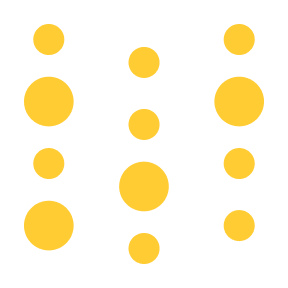
\includegraphics[height=0.8em]{figures/wandb_logo.png}%
  }%
}

%% ----------------------------------------------------------------------
%%    Begin of document + Frontmatter (Roman page numbering)
%% ----------------------------------------------------------------------

\begin{document}

\frontmatter

%% Define the main parameters
\title{Why chose?}
\subtitle{A configurable Transformer Workbench for Multi-Top Quark Classification at the LHC}
\author{Niels ter Linden}

\affiliation{Delft University of Technology} % Cover only
\coverimage{figures/cover.jpg} % Aspect ratio of 2:3 (portrait) recommended
\definecolor{title}{HTML}{4884d6} % Color for cover title

% \makecover

\input{frontmatter/title-report}
\chapter*{Preface}
\addcontentsline{toc}{chapter}{Preface}

\emph{A preface...}

\begin{flushright}
{\makeatletter\itshape
    \@author \\
    Amsterdam, \monthname{} \the\year{}
\makeatother}
\end{flushright}

\input{frontmatter/summary}

\tableofcontents
%\listoffigures
%\listoftables

% \input{frontmatter/nomenclature}

%% ----------------------------------------------------------------------
%%    Mainmatter (Arabic page numbering)
%% ----------------------------------------------------------------------

\mainmatter

\part{Framing}
\chapter{Introduction}
\label{chapter:Introduction}

The


\section{Physics Motivation}
\label{sec:intro_physics_motivation}

\subsection{Multi-top quark production at the LHC}
Four-top-quark production (tttt) is one of the rarest Standard Model processes currently accessible at the LHC, with a small but non-zero predicted cross-section.
Its observation provides a direct handle on the top-quark Yukawa coupling, and deviations from the SM prediction would signal new physics beyond the Standard Model.

\subsection{Why classification matters}
Extracting a signal like tttt from its backgrounds (ttH, ttW, ttZ, ttWW) requires powerful event-level discrimination.
Even modest improvements in classifier performance translate into meaningful gains in signal significance at fixed luminosity.

\cite{collaborationObservationFourtopquarkProduction2023}

\section{Machine Learning Challenge}
\label{sec:intro_ml_challenge}

\subsection{Particle events as variable-length sets}
A collision event is a collection of reconstructed objects --- jets, leptons, and missing transverse energy --- with no natural ordering and varying multiplicity per event.
This set-structured data is awkward for architectures that assume fixed-size inputs or sequential ordering.

\subsection{Transformers as a natural fit}
Self-attention is permutation-equivariant by construction, making transformers well-suited to set-valued inputs.
The attention mechanism can in principle learn to weight particle pairs by their physics relevance without any explicit ordering assumption.

\section{Thesis Statement}
\label{sec:intro_thesis_statement}

\subsection{From single model to configurable workbench}
Rather than producing one optimised classifier, this thesis builds a single modular codebase in which every meaningful architectural decision is exposed as a switchable axis.
We introduce 33 orthogonal architectural axes as the organising principle of the entire experimental programme.

\subsection{Controlled ablation as scientific method}
By varying one axis at a time while holding all others fixed, each experiment becomes a controlled ablation.
The central question is not which configuration achieves the highest AUROC, but what architectural choices matter, and why.

\section{Deliverables}
\label{sec:intro_deliverables}

\subsection{Modular codebase}
The primary engineering output is a Hydra-driven Python package in which every architecture variant is reproducible from a single configuration file.
Any run appearing in this thesis can be regenerated with a single CLI command.

\subsection{Experiment database}
A Weights \& Biases project serves as a structured record of all training runs, storing hyperparameters, metrics, and axis settings in a queryable format.
This database is the raw evidence underlying every quantitative claim in the thesis.

\subsection{Thesis document}
This document is a curated, interpretable distillation of the experiment database: not an exhaustive log of all runs, but a set of focused scientific arguments each anchored to a specific axis group.

\section{Reader's Guide}
\label{sec:intro_readers_guide}

\subsection{Structure of the thesis}
The thesis is organised in three parts: Part~I frames the problem and the workbench (Chapters~2--3); Part~II addresses one focused scientific question per chapter, each mapped to a specific axis group (Chapters~4--9); Part~III synthesises the findings into a recommended configuration and outlook (Chapters~10--11).

\subsection{How to read the results}
Throughout the thesis, AUROC is the primary metric, reported as a seed-averaged mean with error bars.
Axis groups are referred to by their labels (D, A, B, P, H), which correspond directly to config namespaces in the codebase.
Each Part~II chapter is framed by one of three evaluation lenses --- performance, interpretability, or efficiency --- which is stated explicitly at the chapter opening.

\chapter{Dataset and Task Definition}
\label{chapter:dataset}

This chapter describes the dataset used throughout the thesis and defines the classification
tasks evaluated in the experimental chapters. The dataset consists of simulated
proton-proton collision events at $\sqrt{s} = 13\,\text{TeV}$, covering one signal process
($t\bar{t}t\bar{t}$, hereafter four-tops) and four Standard Model (SM) background processes
($t\bar{t}H$, $t\bar{t}W$, $t\bar{t}WW$, $t\bar{t}Z$). Events are encoded as fixed-length
token sequences and stored in HDF5 format. The dataset was received pre-split and used
without modification to the train/validation/test partition. All architectural experiments
in later chapters operate on this single dataset and evaluate binary signal-versus-background
discrimination.

% -------------------------------------------------------------------------
\section{Dataset Provenance}
\label{sec:dataset_provenance}
% -------------------------------------------------------------------------

The dataset originates from two upstream sources. The event generation and detector
simulation pipeline is documented by Builtjes et al.\
\cite{builtjesAttentionStrengthsPhysical2025}, who produced the dataset to study
transformer and graph-based classifiers on multi-top final states. The data format follows
the convention established by the Dark Machines collaboration \cite{Aarrestad:2021oeb}, a
community effort that defined a standardised benchmark format for model-independent LHC
event classification.

Hard-scattering events were generated at leading order using \textsc{MadGraph5\_aMC@NLO}
2.7 with the NNPDF3.1 parton distribution function set and the five-flavour scheme. Parton
showering and hadronisation were performed with \textsc{Pythia}~8.239 using the MLM merging
scheme. Fast detector simulation was carried out with \textsc{Delphes}~3.4.2 using the
ATLAS detector card. An event-generation-level requirement of $H_T > 400\,\text{GeV}$,
summed over parton-level jets, was imposed to increase simulation efficiency for processes
whose reconstructed signal region demands $H_T > 500\,\text{GeV}$. Generated Monte Carlo
samples were converted from ROOT to the Dark Machines CSV format, from which the dataset
used in this thesis was constructed.

The dataset was received in pre-split HDF5 format (\texttt{4tops\_splitted.h5}), with no
train/validation/test partition performed in this work. The exact splitting procedure,
including stratification criterion and random seed, is not documented in the source
materials. \todo{ask supervisor: splitting methodology}

% -------------------------------------------------------------------------
\section{Data Format and Representation}
\label{sec:dataset_format}
% -------------------------------------------------------------------------

Each event in the original CSV follows the Dark Machines line format
\cite{Aarrestad:2021oeb,builtjesAttentionStrengthsPhysical2025}:
\begin{center}
event ID;\enspace process ID;\enspace weight;\enspace
$\|\vec{E}_T^{\,\text{miss}}\|$;\enspace $\phi_{E_T^{\text{miss}}}$;\enspace
$\mathrm{obj}_1,\,E_1,\,p_{T,1},\,\eta_1,\,\phi_1$;\enspace
$\mathrm{obj}_2,\,E_2,\,p_{T,2},\,\eta_2,\,\phi_2$;\enspace$\ldots$
\end{center}
Each reconstructed particle object is characterised by an integer type tag and its
four-momentum $(E,\,p_T,\,\eta,\,\phi)$. Seven object types are defined: jets (\texttt{j},
tag~1), $b$-tagged jets (\texttt{b}, tag~2), positrons (\texttt{e+}, tag~3), electrons
(\texttt{e-}, tag~4), muons (\texttt{mu-}, tag~5), anti-muons (\texttt{mu+}, tag~6), and
photons (\texttt{g}, tag~7). The missing transverse energy magnitude
$\|\vec{E}_T^{\,\text{miss}}\|$ and its azimuthal angle $\phi_{E_T^{\text{miss}}}$ are
stored as two global features shared across all objects in the event.

Because the number of reconstructed objects varies per event, all sequences are
zero-padded to a fixed length of $T = 18$ token slots \cite{Visive:2026mjd}. The value
$T = 18$ corresponds to the largest event in the dataset. A binary attention mask
accompanies each event: padding tokens receive a mask value of zero and are excluded from
attention computations, while real object tokens receive a mask value of one.

The HDF5 file stores each event as a flat row of 92 columns: 18 integer type IDs,
2 global features ($\|\vec{E}_T^{\,\text{miss}}\|$ and $\phi_{E_T^{\text{miss}}}$), and
$18 \times 4 = 72$ continuous kinematic features (one four-momentum per token slot).
The integer type IDs and continuous features are separated at runtime by the data loader.
Before training, the continuous features are normalised using global z-score statistics
computed over the training split only, pooled across all $N_{\text{train}}$ events and all
$T$ token positions simultaneously. This yields one scalar mean and one scalar standard
deviation per feature type ($E$, $p_T$, $\eta$, $\phi$), applied uniformly to every token
slot in every event. No per-position or per-particle-type rescaling is performed.

Across 98.6\% of all thesis training runs, tokens are presented in the order they appear
in the HDF5 file (\texttt{input\_order}). No reordering is applied by the data loader for
these runs. The provenance of the within-event object ordering in the source file is
unknown. \todo{ask supervisor: within-event object ordering in HDF5}

A discrete tokenisation scheme, referred to as AmbreBinning and developed for a subset of
experiments in Chapter~4, maps each continuous four-momentum to a single integer through
independent uniform binning of $p_T$, $\eta$, and $\phi$ (five bins each) combined with
the object-type dimension (125 categories). The combined token index is computed as
$125\,(b_{\text{obj}}-1) + 25\,(b_{p_T}-1) + 5\,(b_\eta-1) + b_\phi$, yielding a
vocabulary of 886 distinct integers. This scheme was inspired by binning strategies
introduced by the thesis supervisor for a related dataset and is not the default
representation; the majority of experiments use continuous four-momentum features directly.

% -------------------------------------------------------------------------
\section{Classification Tasks}
\label{sec:dataset_tasks}
% -------------------------------------------------------------------------

The dataset contains 302,072 events distributed across five SM process classes, split
80/10/10 into training, validation, and test subsets.
Table~\ref{tab:sample_counts} gives the per-class event counts for each split.

\begin{table}[h]
\centering
\caption{Event counts per process class and dataset split. Label codes follow the
convention of Builtjes et al.\ \cite{builtjesAttentionStrengthsPhysical2025}:
1\,=\,$t\bar{t}t\bar{t}$, 2\,=\,$t\bar{t}H$, 3\,=\,$t\bar{t}W$,
4\,=\,$t\bar{t}WW$, 5\,=\,$t\bar{t}Z$.}
\label{tab:sample_counts}
\begin{tabular}{lccccc|c}
\hline
\textbf{Split} & $t\bar{t}t\bar{t}$ & $t\bar{t}H$ & $t\bar{t}W$ & $t\bar{t}WW$ &
$t\bar{t}Z$ & \textbf{Total} \\
\hline
Train & 121{,}359 & 28{,}854 & 30{,}511 & 30{,}461 & 30{,}473 & 241{,}658 \\
Val   & 15{,}266  & 3{,}666  & 3{,}779  & 3{,}760  & 3{,}736  & 30{,}207  \\
Test  & 15{,}375  & 3{,}552  & 3{,}710  & 3{,}779  & 3{,}791  & 30{,}207  \\
\hline
\end{tabular}
\end{table}

The signal process, $t\bar{t}t\bar{t}$, constitutes approximately 50\% of all events. The
four background processes ($t\bar{t}H$, $t\bar{t}W$, $t\bar{t}WW$, $t\bar{t}Z$) each
contribute roughly 10--12\% of the total. This deliberate 1:1 signal-to-background ratio,
chosen by Builtjes et al.\ to balance training \cite{builtjesAttentionStrengthsPhysical2025},
differs markedly from the physical production cross-sections, which strongly favour the
backgrounds, and should be kept in mind when interpreting classifier outputs.

The primary classification task evaluated throughout this thesis is binary discrimination
of $t\bar{t}t\bar{t}$ (label 1) against the combined SM background (labels 2--5). This is
the most physically relevant task: the four-tops process has an extremely small production
cross-section ($\sigma \approx 10\,\text{fb}$ at $\sqrt{s} = 13\,\text{TeV}$), and its
first observation by ATLAS required careful discrimination from a large and topologically
similar SM background \cite{collaborationObservationFourtopquarkProduction2023}. The task
is challenging because each top quark decays almost exclusively via $t \to Wb$, so four-top
events produce high-multiplicity final states with 0--4 leptons and 4--12 jets, including
four $b$-jets. Background processes such as $t\bar{t}WW$ and $t\bar{t}Z$ produce
comparably complex topologies. The classifier must therefore exploit subtle differences in
object multiplicity, kinematic correlations, and $b$-jet content to separate signal from
background.

All architectural ablations in Chapters~4--8 evaluate this binary task, reporting area
under the receiver operating characteristic curve (AUROC) and background rejection at fixed
signal efficiency as primary metrics.

\chapter{The Workbench: Architecture and Axes}

\section{Design philosophy}

Rather than committing to a single architecture, the workbench exposes
every meaningful design choice as a switchable configuration parameter.
This makes fair comparison possible by construction: when one axis
changes, everything else is held fixed, so any observed difference in
AUROC is attributable to that choice alone. The entire architecture is
specified by a Hydra configuration tree, where each axis corresponds to
a named key in a structured YAML hierarchy. Any run in the experiment
database can be regenerated from a single command-line invocation.

\section{The base transformer}

The base model follows the standard transformer encoder pipeline:
particle tokens are embedded into a fixed-dimensional space, passed
through a stack of attention-plus-FFN blocks, aggregated into a single
event-level vector by a pooling operation, and classified by a head
network. This skeleton is fixed across all experiments; the axes
control what happens inside each stage.

Each particle token, a raw kinematic vector plus an optional
particle-type identifier, is projected into the model dimension $d$
by a linear embedding layer. The encoder consists of $L$ identical
blocks, each containing a multi-head self-attention layer followed by
a position-wise feed-forward network, with residual connections and
normalisation at positions controlled by axes A1 and A2. The pooled
vector is passed to a classifier head that produces the final logit.

\section{Axis groups}

The axes are organised into ten groups. Groups G and D define the
experimental conditions and data treatment. Groups T, E, P, A, F, B,
and C define the architecture. Group H sets model capacity. Three
cross-cutting shared parameter blocks (§K, §M, §S) are consumed by
multiple modules simultaneously and are documented at the end of this
section. Groups §R and §L cover training protocol and logging
respectively and are not architectural axes.

% ──────────────────────────────────────────────
\subsection*{G \quad Study framing}

G axes define what is being classified and with which model family.
They are not architectural choices and are not varied in the ablation
programme; they set the experimental conditions under which all other
axes are evaluated.

\textbf{G01 -- Task type.} Selects the training loop: supervised
classification or anomaly detection (autoencoder, GAN-AE, diffusion-AE).
This thesis focuses exclusively on supervised classification;
the anomaly detection loops are available in the workbench but not
studied here.

\textbf{G02 -- Model family.} Selects the model architecture family:
transformer, MLP, BDT, or autoencoder. All Part II chapters use the
transformer family; the BDT appears only in Ch.\,8 as a surrogate
model for configuration prediction, not as a classifier.

\textbf{G03 -- Classification task.} Defines which processes are
treated as signal and background. Five processes are available:
four-top-quark production ($tttt$), associated production with a Higgs
boson ($ttH$), with a $W$ boson ($ttW$), with two $W$ bosons ($ttWW$),
and with a $Z$ boson ($ttZ$). Three task definitions are used in this
thesis: $tttt$ vs.\ combined background ($ttH + ttW + ttWW + ttZ$) as
the primary task, $tttt$ vs.\ $ttH$ as a harder secondary task, and
all-five multiclass as an exploratory task.

% ──────────────────────────────────────────────
\subsection*{D \quad Data treatment}

D axes control what the model sees before any architectural processing.

\textbf{D01 -- Feature set.} Selects which kinematic features are
included in each token. The default is the four-feature set
(E, Pt, $\eta$, $\phi$); energy can be omitted to test whether the
model relies on explicit $E$ or whether Pt, $\eta$, and $\phi$ already
provide sufficient kinematic information.

\textbf{D02 -- MET treatment.} Controls whether missing transverse
energy is excluded or included as an event-level global. Tests how much
the invisible neutrino system contributes beyond the particle tokens.

\textbf{D03 -- Token ordering.} Sets whether tokens are presented in
input order, sorted by decreasing Pt, or randomly shuffled per event.
Tests whether the model exploits ordering as an implicit positional
signal.

% ──────────────────────────────────────────────
\subsection*{T \quad Tokenizer}

T axes control how raw particle features are converted into token
embeddings.

\textbf{T1 -- Tokenizer family.} Selects between \texttt{raw}
(kinematics only), \texttt{identity} (kinematics plus an explicit
particle-type label), and \texttt{binned} (discrete token, no
continuous features). Tests whether explicit particle identity is
necessary or recoverable from kinematics alone.

\textbf{T1-a -- PID embedding mode.} When T1 = \texttt{identity},
selects how the particle-type label is encoded: \texttt{learned},
\texttt{one\_hot}, or \texttt{fixed\_random}. Tests whether particle
identity needs a learned geometry or only a categorical code.

\textbf{T1-b -- PID embedding dimension.} Sets the capacity of the
PID embedding to 8, 16, or 32 dimensions. Tests the trade-off between
representational capacity and overfitting for the type sub-embedding.

% ──────────────────────────────────────────────
\subsection*{E \quad Positional encoding}

E axes control how position information is injected into the token
stream.

\textbf{E1 -- PE type.} Selects among \texttt{none},
\texttt{sinusoidal}, \texttt{learned}, and \texttt{rotary}. Tests
whether injecting position information helps a set-based classifier at
all.

\textbf{E1-a -- PE space.} Controls whether the positional signal is
applied before or after the input projection. Prerequisite: E1
$\in$ \{sinusoidal, learned\}.

\textbf{E1-a1 -- PE dimension mask.} Allows the positional encoding to
act selectively on a subset of feature dimensions. Prerequisite:
E1-a = \texttt{token}.

% ──────────────────────────────────────────────
\subsection*{P \quad Pre-encoder modules}

P axes add optional modules applied to raw particle features before the
main transformer encoder. Both require T1 $\in$ \{raw, identity\}.

\textbf{P1 -- Nodewise mass patch.} Optionally enriches each token with
invariant-mass features computed from its $k$-nearest neighbours in
Lorentz space, following Li et al. Tests whether explicit local mass
structure before the encoder improves token representations. Requires
D01 to include energy (index 0).

\textbf{P2 -- MIA pre-encoder.} Optionally inserts MIParT-style
interaction-attention blocks before the main encoder, where attention
is driven by pairwise interaction features rather than query-key
similarity. Tests whether physics-driven message passing as a
pre-encoder stage adds information beyond standard self-attention.

\textbf{P2-a -- MIA placement.} Controls whether MIA blocks are
prepended or appended relative to the main encoder. Prerequisite:
P2 = \texttt{true}.

% ──────────────────────────────────────────────
\subsection*{A \quad Attention and encoder block}

A axes control the internal design of each encoder block.

\textbf{A1 -- Normalisation policy.} Selects pre-norm, post-norm, or
NormFormer placement of layer normalisation within each block. Tests
whether normalisation position affects training stability for
particle-level inputs.

\textbf{A2 -- Normalisation type.} Chooses between LayerNorm and
RMSNorm. Tests whether removing the mean-subtraction step improves
efficiency without degrading performance.

\textbf{A3 -- Attention type.} Selects standard multi-head attention
or differential attention, which computes the difference of two softmax
maps to suppress diffuse attention patterns. Tests whether this
mechanism transfers from NLP to particle classification.

\textbf{A3-a -- Differential bias mode.} When A3 =
\texttt{differential}, controls how additive physics biases interact
with the two attention branches: \texttt{none}, \texttt{shared}, or
\texttt{split}. Prerequisite: A3 = \texttt{differential}.

\textbf{A4 -- Attention-internal normalisation.} Optionally applies
LayerNorm or RMSNorm per head after the weighted sum, before head
merging. Tests whether per-head normalisation stabilises attention
output scales. Applies to both standard and differential attention.

\textbf{A5 -- Causal masking.} Optionally applies an autoregressive
mask to the attention matrix. Tests whether imposing sequential
structure on an inherently unordered set of particles hurts, helps,
or is neutral.

% ──────────────────────────────────────────────
\subsection*{F \quad Encoder FFN realization}

F axes control the feed-forward network inside each encoder block. The
effective realization follows a priority rule: MoE $>$ KAN $>$ standard.

\textbf{F1 -- FFN realization.} Selects between a standard two-layer
MLP, a Kolmogorov--Arnold Network (KAN), and a Mixture-of-Experts (MoE)
FFN. Tests whether learnable spline activations or conditional
computation improve per-token transformations.

\textbf{F1-a -- KAN FFN variant.} When F1 = \texttt{kan}, selects
among \texttt{hybrid}, \texttt{bottleneck}, and \texttt{pure}
architectures. Prerequisite: F1 = \texttt{kan}.

\textbf{F1-b -- MoE scope.} Controls whether expert routing applies
to encoder FFNs, the classifier head, or both. Prerequisite:
F1 = \texttt{moe}.

% ──────────────────────────────────────────────
\subsection*{B \quad Physics-informed attention biases}

B axes inject physics structure as additive biases on the attention
logits. All families require T1 $\in$ \{raw, identity\} and share a
zero-initialised scalar gate, so adding any bias leaves the baseline
unchanged at initialisation. Multiple families can be active
simultaneously using \texttt{+} notation.

\textbf{B1 -- Bias activation set.} The master switch selecting which
bias families are active: \texttt{lorentz\_scalar},
\texttt{typepair\_kinematic}, \texttt{sm\_interaction},
\texttt{global\_conditioned}, or combinations thereof.

\textbf{B1-L1 -- Lorentz feature set.} Selects the subset of pairwise
Lorentz-invariant features fed into the bias network, from the minimal
set \{m$^2$, $\Delta R$\} through the MIParT basis to the full feature
set. Active when \texttt{lorentz\_scalar} $\in$ B1.

\textbf{B1-L2 -- Lorentz MLP type.} Selects whether the network
mapping Lorentz features to bias scores uses a standard MLP or a KAN.
Active when \texttt{lorentz\_scalar} $\in$ B1.

\textbf{B1-L5 -- Lorentz sparse gating.} Adds per-feature sigmoid
gates providing a direct measure of learned feature importance. Active
when \texttt{lorentz\_scalar} $\in$ B1.

\textbf{B1-T2 -- Type-pair initialisation.} Controls how the learnable
$N_\text{type} \times N_\text{type}$ interaction table is initialised:
from scratch, from a binary SM mask, or from fixed SM coupling
constants. Active when \texttt{typepair\_kinematic} $\in$ B1.

\textbf{B1-T3 -- Type-pair freeze.} Controls whether the type-pair
table is frozen after initialisation or remains trainable. Tests
whether the table is better used as a fixed physics prior or a
learnable parameter. Active when \texttt{typepair\_kinematic} $\in$ B1.

\textbf{B1-S1 -- SM interaction mode.} Selects the fidelity of the SM
interaction prior: \texttt{binary}, \texttt{fixed\_coupling}, or
\texttt{running\_coupling}. Active when \texttt{sm\_interaction}
$\in$ B1.

\textbf{B1-G1 -- Global-conditioned mode.} Controls how MET modulates
pairwise attention biases: as a global scale factor or as a directional
signal. Requires D02 = \texttt{true}. Active when
\texttt{global\_conditioned} $\in$ B1.

% ──────────────────────────────────────────────
\subsection*{C \quad Classifier head}

C axes control the final mapping from the pooled event representation
to class logits.

\textbf{C1 -- Head realization.} Selects between a \texttt{linear}
head, a \texttt{kan} head, and a \texttt{moe} head. Tests whether
specialised nonlinearities or conditional computation at the decision
boundary improve discrimination.

\textbf{C2 -- Pooling strategy.} Selects how the token sequence is
aggregated into a single event-level vector: \texttt{cls} token,
\texttt{mean} pooling, or \texttt{max} pooling. Placed here because
pooling is logically part of the readout stage rather than the encoder
block.

% ──────────────────────────────────────────────
\subsection*{H \quad Model-size hyperparameters}

H axes set model capacity and are not architectural design choices in
the sense of the other groups. They are tracked separately and are the
primary axis of variation in Ch.\,9. The convenience key
\texttt{model\_size\_key} bundles dim ($d$), depth ($L$), heads, and
FFN hidden dim into named presets spanning roughly 50k to 4M
parameters.

% ──────────────────────────────────────────────
\subsection*{Cross-cutting blocks: §K, §M, §S}

Three shared parameter blocks are consumed simultaneously by multiple
modules. §K (KAN hyperparameters: grid size, spline order, grid range)
affects every active KAN module, including the encoder FFN, classifier
head, and Lorentz bias network. §M (MoE hyperparameters: number of
experts, top-k, routing level) affects all active MoE sites. §S (shared
pairwise backbone) computes the pairwise feature matrix $F_{ij}$ once
per forward pass and shares it across all active B1 families and the
MIA pre-encoder.

\section{Experimental methodology}

Each axis is studied in isolation: one axis is varied across its
settings while all others are held at their defaults, forming an
orthogonal sweep. This ensures observed differences are attributable to
the axis under study and keeps the number of required experiments
linear in the number of axes rather than exponential.

Every result reported in this thesis is averaged over at least three
independently seeded runs, with error bars representing the standard
deviation across seeds. The area under the ROC curve (AUROC) is the
primary evaluation metric throughout: it measures the probability that
the classifier assigns a higher score to a signal event than to a
background event, and is threshold-independent. Signal efficiency at
fixed background rejection is reported as a complementary metric in
selected chapters.

All runs are tracked in a Weights \& Biases project where every axis
setting, hyperparameter, and evaluation metric is logged under a
structured key scheme mirroring the axis reference directly.


\part{Thesis Questions}
% ============================================================
% CHAPTER 4: BEST INPUT REPRESENTATION
% Draft status: full skeleton with real numbers where available.
% Prose is intentionally skeletal — expand per section notes.
% Figures marked [HAVE] exist; [NEED] require new inference/plots.
% ============================================================

\chapter{Best Input Representation}
\label{ch:input-repr}

% --- SECTION INTRO NOTE ---
% 1 paragraph: frame the question as "before the transformer sees anything,
%   choices have already been made." Name the six axes: T1, T1-a, T1-b, D01,
%   D02, D03. State the two lenses: (1) performance (what helps?) and (2)
%   interpretability (what does the gap reveal about the physics?).
% Mention that the chapter baseline (Table~\ref{tab:ch4-baseline}) flows
%   forward into every subsequent chapter.

Before the transformer processes a single attention operation,
several choices have already shaped the information available to it:
whether each particle token carries an additional explicit identity label or only
its four-vector with $p_t$ and $E$, $\eta$ and $\phi$ (T1), and if it does carry the Particle ID
how that label is encoded (T1-a, T1-b),
which kinematic components are included (D01),
whether missing transverse energy is present as an additional token (D02),
and in what order the tokens arrive (D03).
This chapter asks which of these choices matter, and why.
The experimental programme consists of two sweeps:
Experiment~4A varies the tokenizer family and PID encoding,
and Experiment~4B varies the feature set, MET inclusion, and token ordering.
All other axes are held at the canonical defaults defined in
Chapter~\ref{ch:workbench}.

% ============================================================
\section{Tokenizer family and PID encoding (Exp.\ 4A)}
\label{sec:exp4a}
% ============================================================

% --- SECTION INTRO NOTE ---
% 1 short paragraph: the core question is whether particle identity is
%   recoverable from kinematics alone. State that we test three families
%   (raw, identity, binned) and, within identity, sweep T1-a (pid_mode)
%   and T1-b (id_embed_dim). Refer to Table~\ref{tab:exp4a}.

\begin{table}[h]
\centering
\small
\begin{tabular}{lllr}
\toprule
Factor & Values & Applies to & $n_\text{configs}$ \\
\midrule
T1 — Tokenizer family & \texttt{raw} & all & 1 \\
                       & \texttt{binned} & all & 1 \\
                       & \texttt{identity} & — & — \\
\quad T1-a — PID mode & \texttt{one\_hot}, \texttt{fixed\_random}, \texttt{learned} & identity & 3 \\
\quad T1-b — PID dim  & 8, 16, 32 & identity & 3 \\
\midrule
\multicolumn{3}{l}{Unique configurations} & 11 \\
\multicolumn{3}{l}{Seeds per configuration} & 3 \\
\multicolumn{3}{l}{\textbf{Total runs}} & \textbf{33} \\
\bottomrule
\end{tabular}
\caption{Experiment 4A sweep design.
All axes not listed are held at the canonical defaults (Chapter~\ref{ch:workbench}).
D01\,=\,\texttt{[0,1,2,3]}, D02\,=\,\texttt{false}, D03\,=\,\texttt{input\_order}.}
\label{tab:exp4a}
\end{table}

% -------------------------------------------------------
\subsection{Tokenizer family comparison}
\label{sec:exp4a-family}
% -------------------------------------------------------

% --- NOTE ---
% Core argument (2–3 sentences): identity outperforms raw by +0.031 AUROC
%   and binned by +0.040. The ROC curves confirm this is a uniform lift,
%   not threshold-specific. The training dynamics (Fig~\ref{fig:val-auroc-tokenizer})
%   add mechanistic colour: binned overfits hard (peak ~epoch 4, collapses to
%   0.74); raw plateaus and is stable; identity converges high and stays high.
%   Interpretation: binned discards the continuous kinematic information
%   entirely (only discrete bin IDs remain), which is too lossy for this task.
%   raw retains kinematics but cannot signal particle type; identity provides both.
% Keep this section to ~1 paragraph of argument + the two figures.

The \texttt{identity} tokenizer achieves a mean test AUROC of $0.835$
across all T1-a/T1-b configurations,
compared with $0.804$ for \texttt{raw} ($+0.031$)
and $0.795$ for \texttt{binned} ($+0.040$).

% [HAVE] Figure: AUROC bar by tokenizer family
\begin{figure}[h]
\centering
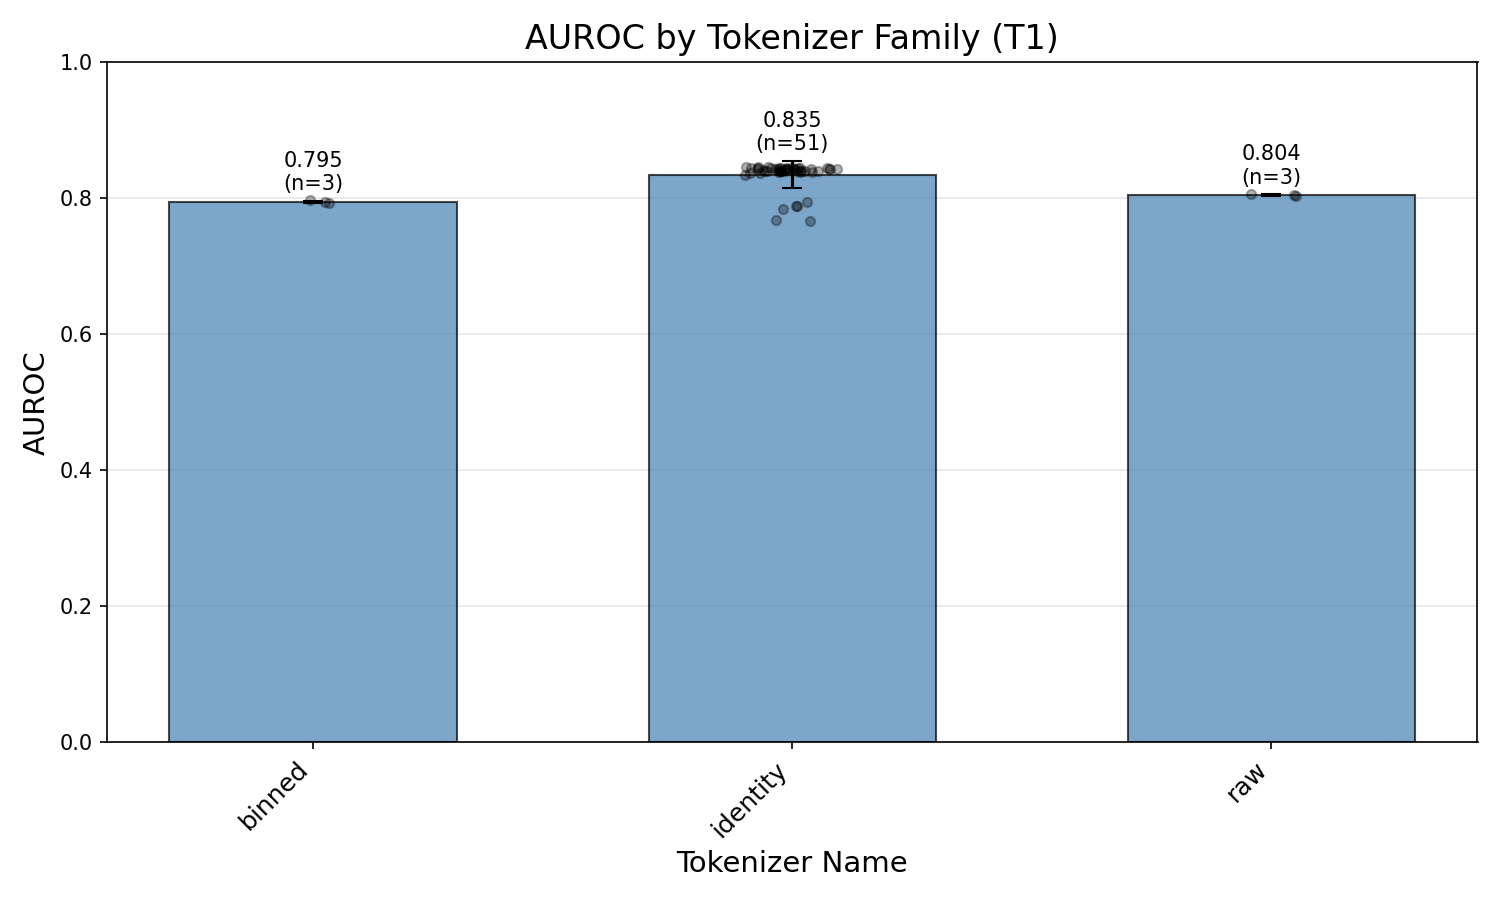
\includegraphics[width=0.65\textwidth]{figures/ch4/figure-auroc_bar_by_tokenizer.png}
\caption{Mean test AUROC by tokenizer family (T1).
Error bars show one standard deviation over seeds.
The \texttt{identity} family pools all T1-a and T1-b configurations ($n=51$);
\texttt{raw} and \texttt{binned} each have $n=3$ (three seeds).
% NOTE: consider regenerating with median + IQR, or separating identity
%   sub-configurations to avoid conflating the learned/dim=8 outlier.
}
\label{fig:auroc-bar-tokenizer}
\end{figure}

% [HAVE] Figure: ROC curves by tokenizer family
\begin{figure}[h]
\centering
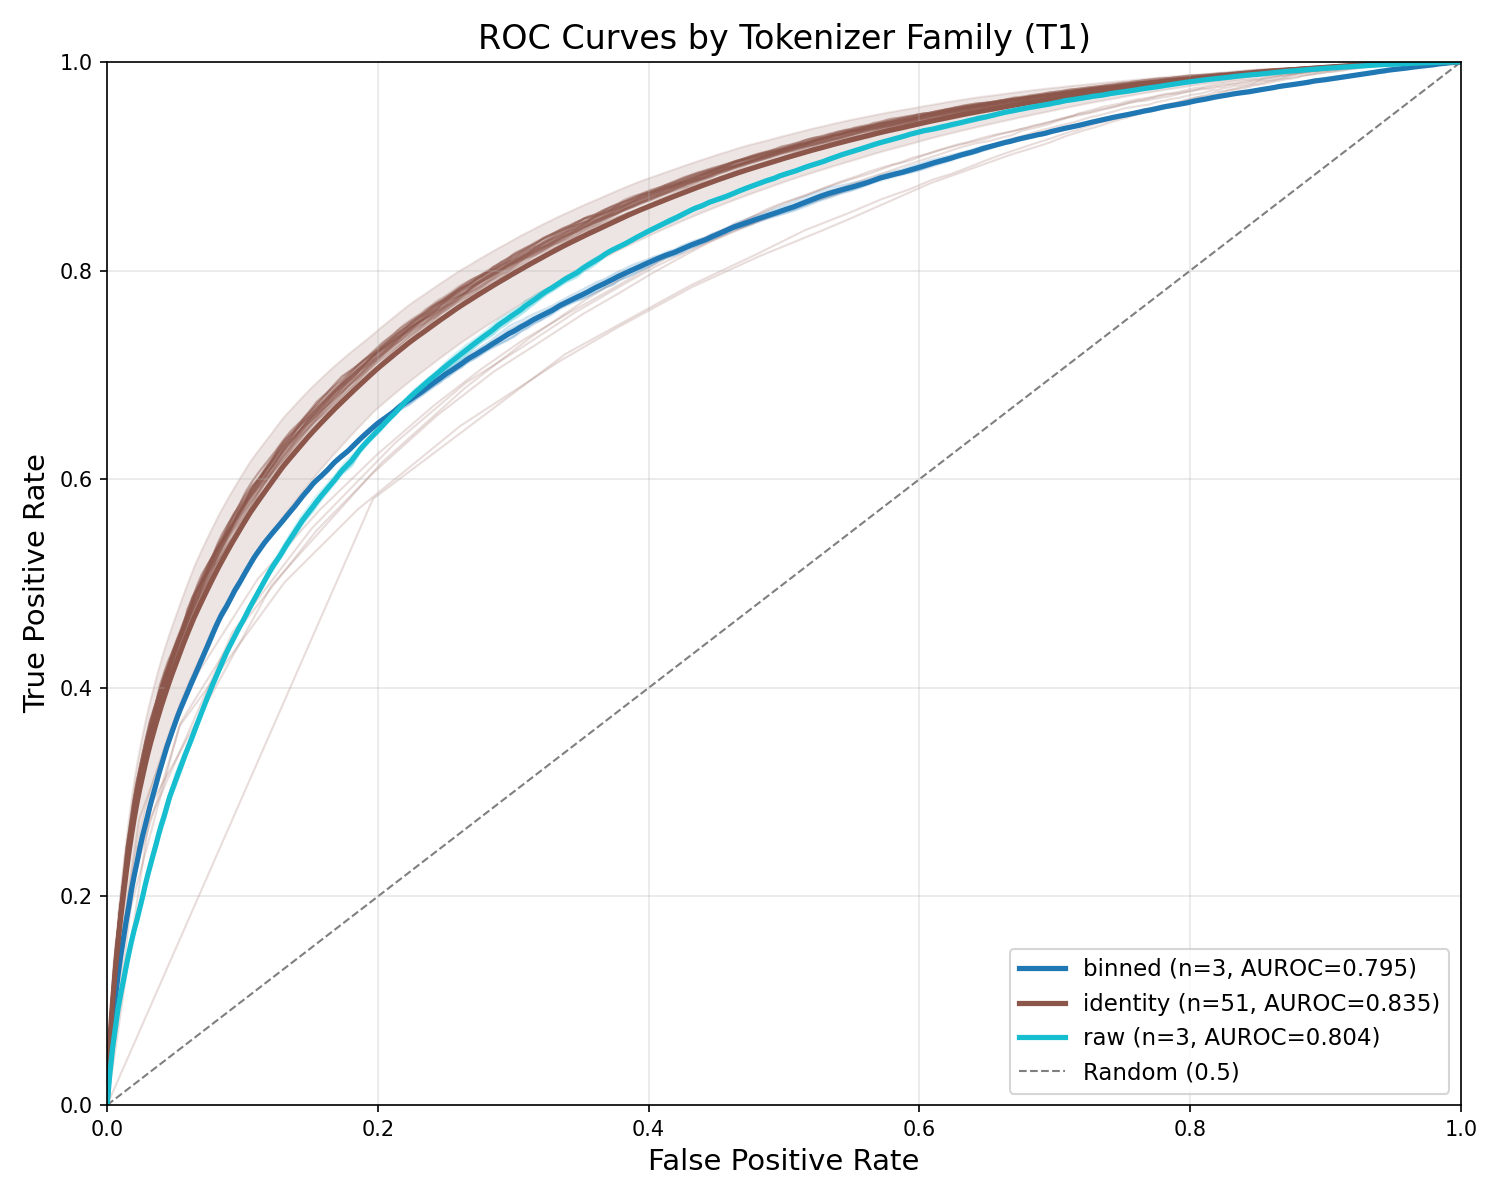
\includegraphics[width=0.65\textwidth]{figures/ch4/figure-roc_curves_by_tokenizer.png}
\caption{ROC curves by tokenizer family.
Shaded bands span the seed spread for \texttt{identity};
\texttt{raw} and \texttt{binned} show individual seed curves.
The identity advantage is uniform across the full operating range.}
\label{fig:roc-tokenizer}
\end{figure}

% [HAVE] Figure: validation AUROC training curves by tokenizer family
\begin{figure}[h]
\centering
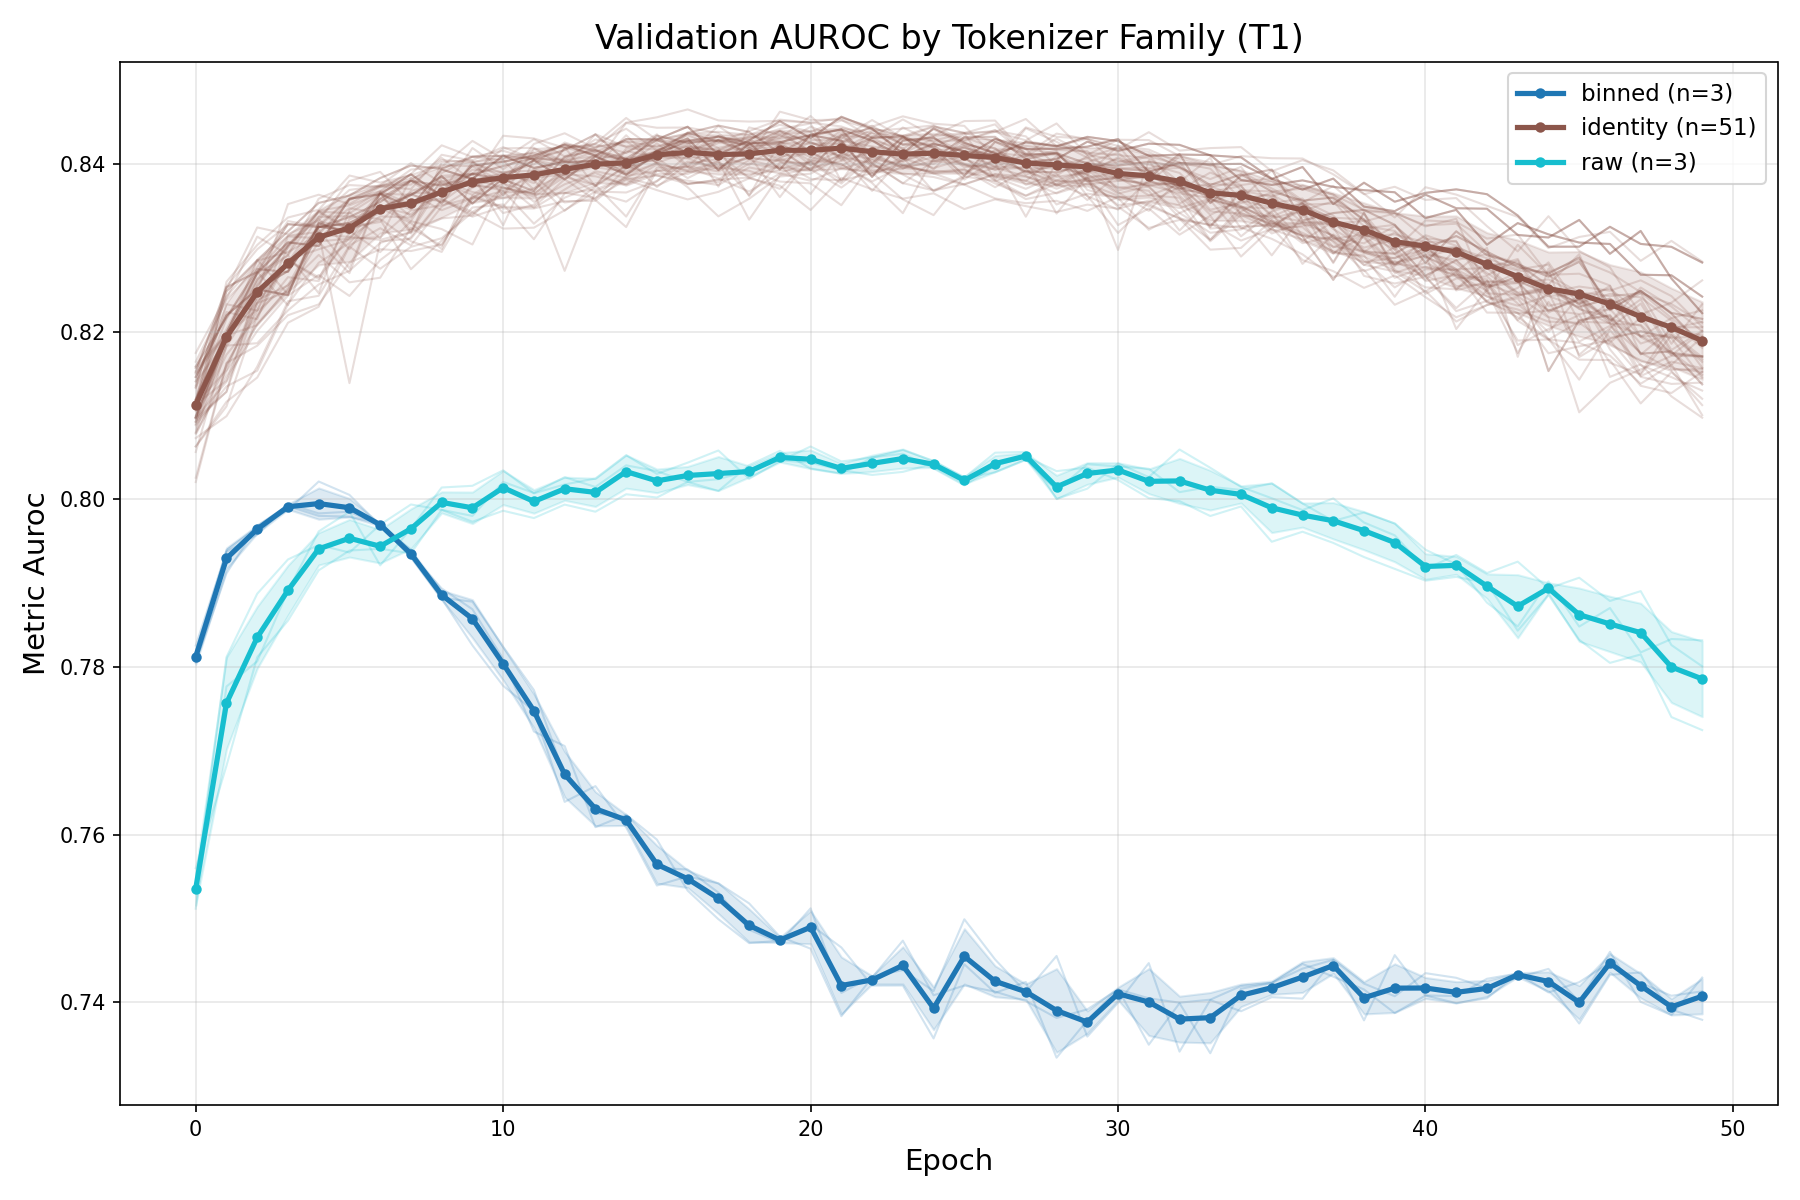
\includegraphics[width=0.65\textwidth]{figures/ch4/figure-val_auroc_by_tokenizer.png}
\caption{Validation AUROC over training epochs by tokenizer family.
\texttt{binned} peaks near epoch 4 and subsequently collapses, indicating
rapid overfitting once the discrete token vocabulary is memorised.
\texttt{raw} converges stably but at a lower plateau.
\texttt{identity} converges to a higher plateau and degrades slowly beyond
peak, consistent with mild overtraining at 50 epochs.
% NOTE: may want to crop x-axis to 0--35 epochs to focus on the interesting region.
}
\label{fig:val-auroc-tokenizer}
\end{figure}

% -------------------------------------------------------
\subsection{PID encoding mode and embedding dimension (T1-a, T1-b)}
\label{sec:exp4a-pid}
% -------------------------------------------------------

% --- NOTE ---
% This subsection has a trap in the data that must be explained honestly.
%
% The 1D bar for T1-a (Fig~\ref{fig:auroc-bar-pid-mode}) shows:
%   one_hot=0.844, fixed_random=0.841, learned=0.825.
% This naively reads as "learned is worse." But the heatmap
%   (Fig~\ref{fig:heatmap-pid-dim}) reveals the confound:
%   learned at dim=8 collapses to 0.8275, while at dim=16/32 it
%   recovers to 0.840+. The learned bar is depressed because dim=8
%   runs dominate the learned sample (n=39 vs n=9 for others).
%
% The fair comparison (all modes at dim=16 or dim=32) shows all three
%   modes within ~0.003 of each other.
%
% Interpretation: one_hot and fixed_random do not need to learn the
%   embedding geometry, so dim=8 is sufficient. Learned embeddings
%   at dim=8 are under-specified: 8 dimensions to learn a meaningful
%   geometry over the particle type vocabulary is tight, and optimisation
%   for the downstream task may sacrifice embedding quality.
%
% Practical conclusion: one_hot at dim=8 (or any dim, since one_hot is
%   dimension-agnostic by construction) is the most robust and parameter-efficient
%   choice. Use this as Ch5+ baseline.
%
% Write ~2 paragraphs: (1) explain the 1D bar trap, (2) read the heatmap correctly.

% [HAVE] Figure: AUROC bar by PID mode (1D marginal — misleading, needs caveat)
\begin{figure}[h]
\centering
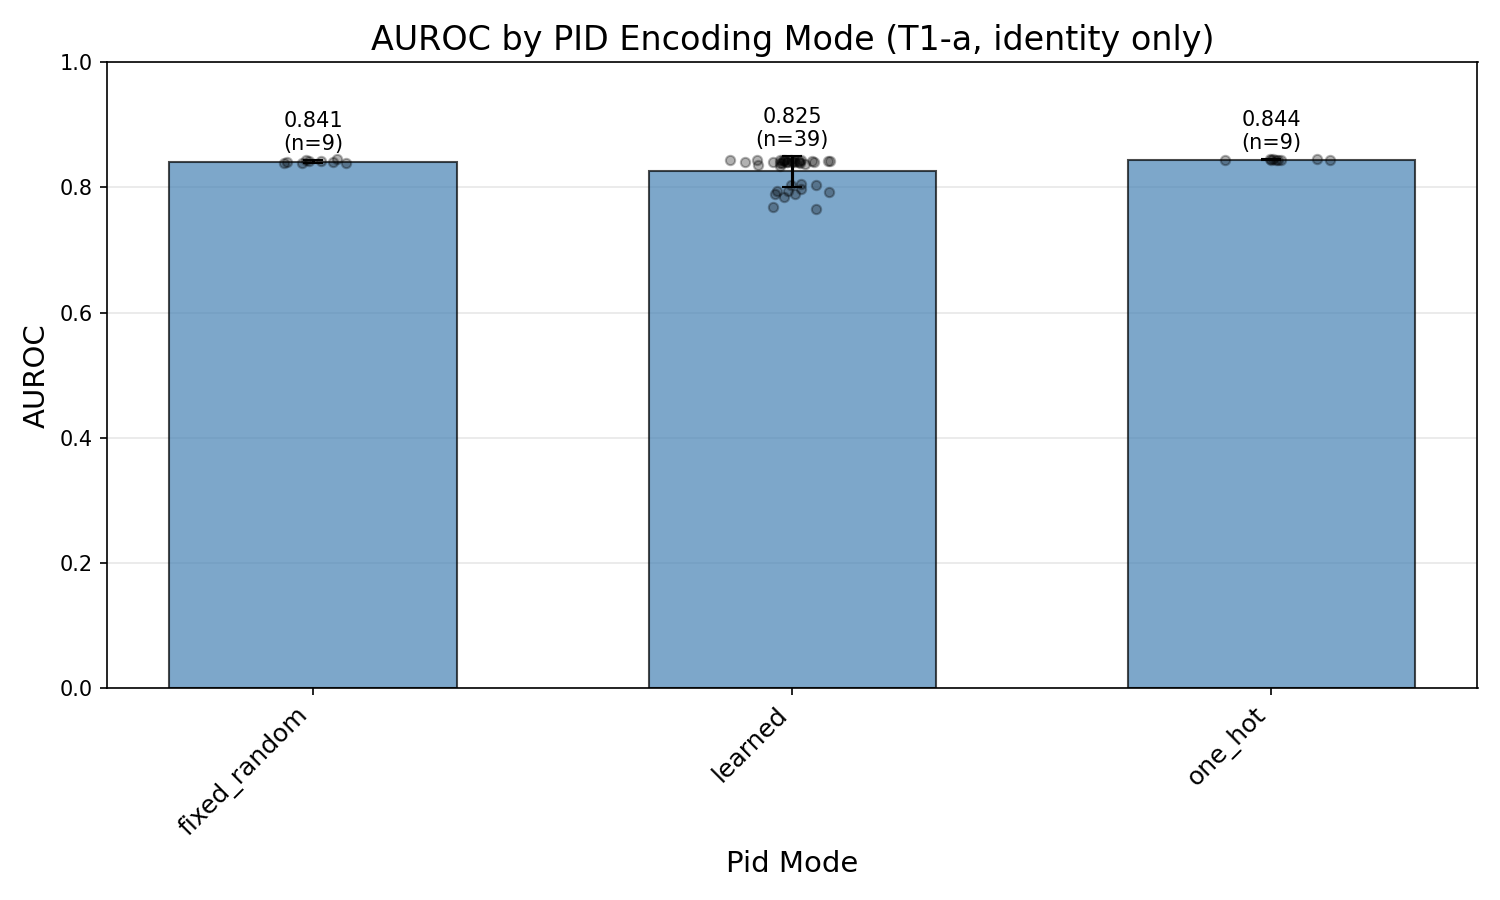
\includegraphics[width=0.65\textwidth]{figures/ch4/figure-auroc_bar_by_pid_mode.png}
\caption{Mean test AUROC by PID encoding mode (T1-a), pooled over all T1-b
embedding dimensions.
The apparent underperformance of \texttt{learned} is a confound:
the \texttt{learned} sample is dominated by dim=8 runs ($n=39$ of $n=57$),
which perform poorly (see Figure~\ref{fig:heatmap-pid-dim}).
At dim\,$\geq$\,16, all three modes are within $0.003$ AUROC of each other.
% NOTE: consider replacing this figure with one that holds dim fixed,
%   or annotating it with a dashed line for "learned at dim=16+."
}
\label{fig:auroc-bar-pid-mode}
\end{figure}

% [HAVE] Figure: AUROC heatmap T1-a x T1-b
\begin{figure}[h]
\centering
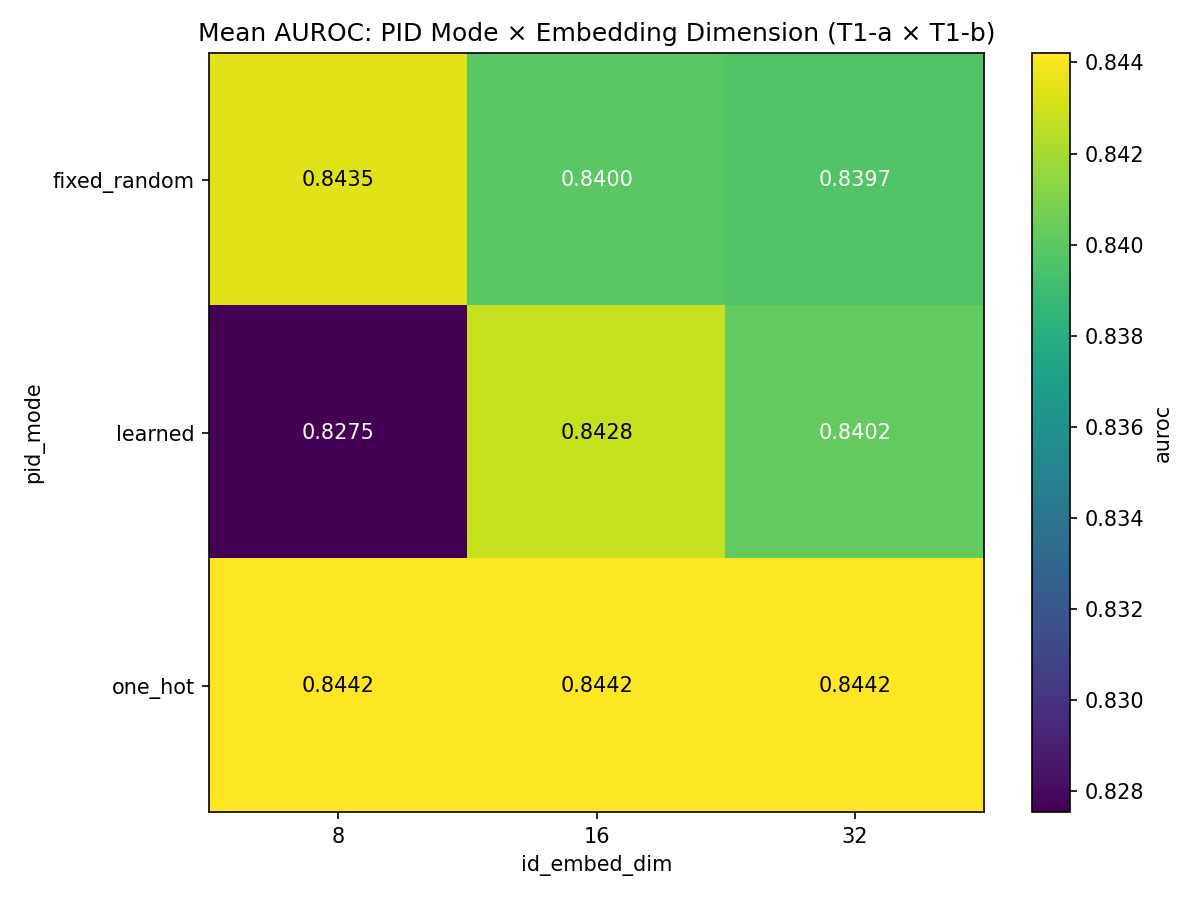
\includegraphics[width=0.72\textwidth]{figures/ch4/figure-auroc_heatmap_pid_mode_x_embed_dim.png}
\caption{Mean test AUROC as a function of PID encoding mode (T1-a) and
embedding dimension (T1-b), for the \texttt{identity} tokenizer family.
\texttt{one\_hot} is invariant to dimension by construction
(the embedding dimension is overridden to the number of particle types).
\texttt{fixed\_random} performs well at all dimensions.
\texttt{learned} at dim=8 is the clear outlier (0.8275);
at dim$\,\geq\,$16 it recovers to parity with the other modes.}
\label{fig:heatmap-pid-dim}
\end{figure}

% [HAVE] Figure: AUROC bar by embedding dimension (1D marginal)
\begin{figure}[h]
\centering
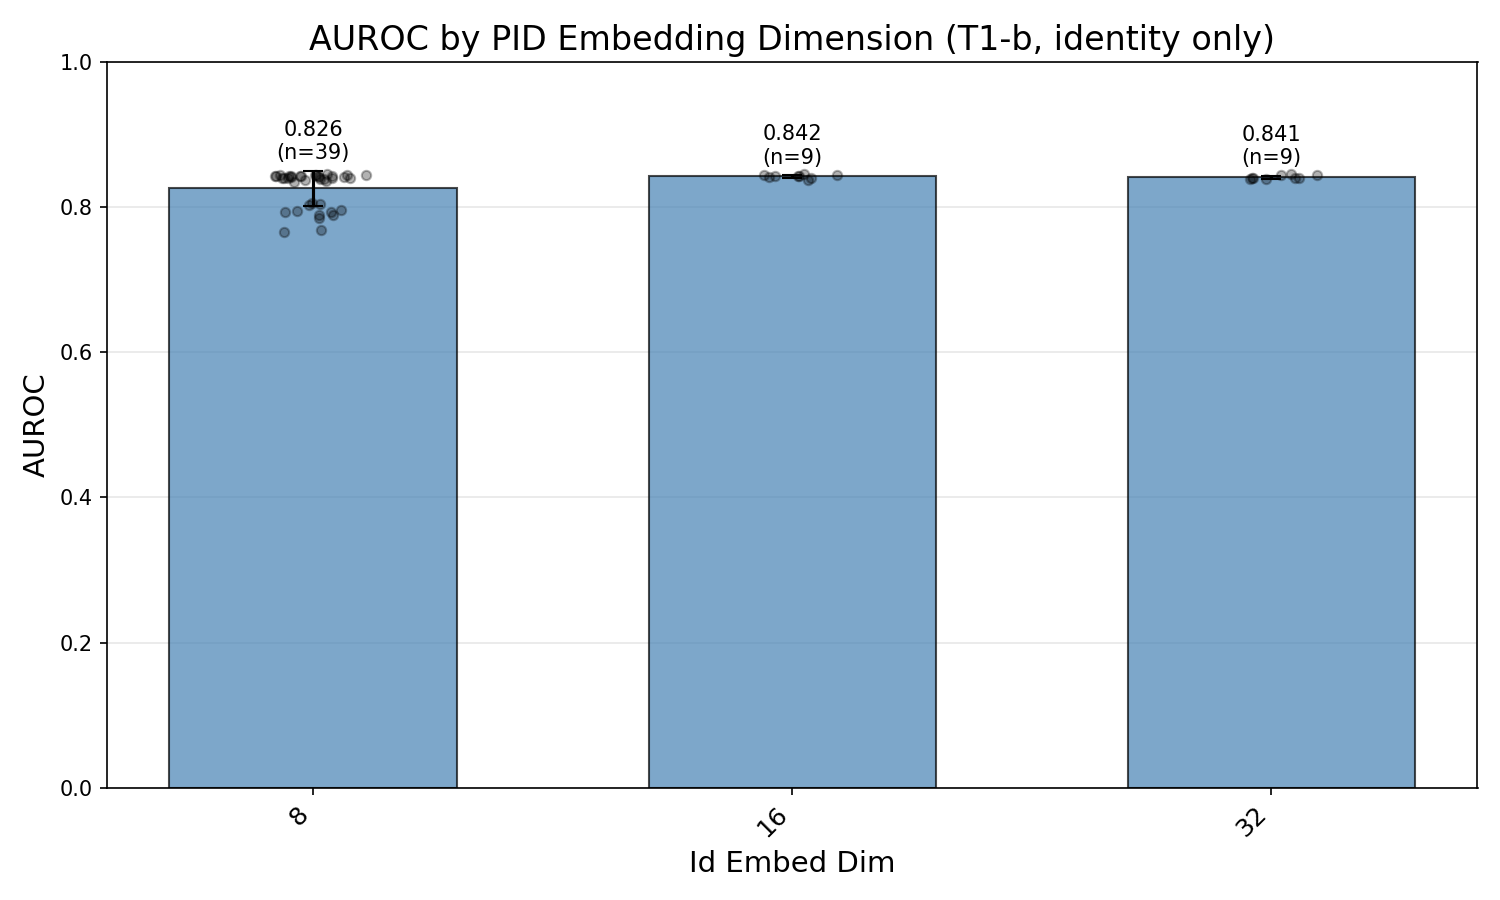
\includegraphics[width=0.65\textwidth]{figures/ch4/figure-auroc_bar_by_id_embed_dim.png}
\caption{Mean test AUROC by PID embedding dimension (T1-b), pooled over T1-a modes.
The dim=8 average ($0.826$) is depressed by the \texttt{learned}/dim=8 outlier.
Dim=16 ($0.842$) and dim=32 ($0.841$) are effectively equivalent.
% NOTE: same caveat as Fig~\ref{fig:auroc-bar-pid-mode}; this 1D view is
%   misleading without the heatmap context.
}
\label{fig:auroc-bar-dim}
\end{figure}

% [NEED] Optional figure: t-SNE or UMAP of the learned PID embedding vectors
%   coloured by particle type. Would show whether 8 dimensions produce
%   a collapsed/entangled geometry vs 16+ producing clean separation.
%   Low priority — only add if the geometry story is interesting.
% \begin{figure}[h]
% \centering
% \includegraphics[width=0.65\textwidth]{figures/ch4/figure-tsne_pid_embeddings.png}
% \caption{[PLACEHOLDER] t-SNE projection of learned PID embedding vectors
%   at dim=8 (left) and dim=16 (right), coloured by particle type.}
% \label{fig:tsne-pid}
% \end{figure}

% -------------------------------------------------------
\subsection{Failure analysis: what does PID unlock?}
\label{sec:exp4a-failure}
% -------------------------------------------------------

% --- NOTE ---
% This is the interpretability payoff of the chapter. Keep it tight.
%
% The failure analysis compares per-event predictions between the best
%   raw model and the best identity model on the held-out test set
%   (N=30,207 events).
%
% Numbers from the figure:
%   both_correct:   20,121  (66.6%)
%   identity_fixed: 2,515   (8.3%)  — PID helped
%   raw_fixed:      2,014   (6.7%)  — PID hurt
%   both_wrong:     5,557   (18.4%)
%   net gain:       +501 events
%
% Argument to make:
%   (1) The vast majority of events are correctly handled by both or neither.
%       PID changes the outcome for ~15% of events total.
%   (2) The net asymmetry (8.3% vs 6.7%) is real but modest. PID is not
%       universally helpful: in 6.7% of events, removing the explicit label
%       actually improves classification. This is worth one sentence of
%       explanation: those events may have ambiguous or mislabelled type
%       information, or the raw model learns a compensating heuristic.
%   (3) The scatter plot (left panel) shows that identity-fixed events
%       (blue) sit systematically above the diagonal — the identity model
%       pushes them toward higher signal score. The raw-fixed events (orange)
%       sit below.
%   (4) 18.4% of events are wrong for both: these define the irreducible
%       difficulty ceiling of the task regardless of tokenizer.
%
% [WANT] An additional breakdown: of the 2,515 events where PID helped,
%   what is their kinematic profile? Hypothesis: they are events where
%   particle type is ambiguous from kinematics (e.g., b-jets and light jets
%   at similar pT). If the report already extracted event-level features for
%   the flipped events, this could be a simple 1D histogram of, e.g.,
%   jet multiplicity or leading jet pT for the four categories.
%   Flag for potential new inference run if not available.

Of the $30{,}207$ test events,
$66.6\%$ are classified correctly by both tokenizers,
and $18.4\%$ are wrong for both,
defining the task's irreducible floor given this model capacity and data.
In the remaining $15\%$,
the tokenizer choice determines the outcome:
$8.3\%$ of events are fixed by adding an explicit particle-type label
(PID helped),
while $6.7\%$ are misclassified when PID is available but correct without it
(PID hurt),
giving a net gain of $501$ events.

\begin{figure}[h]
\centering
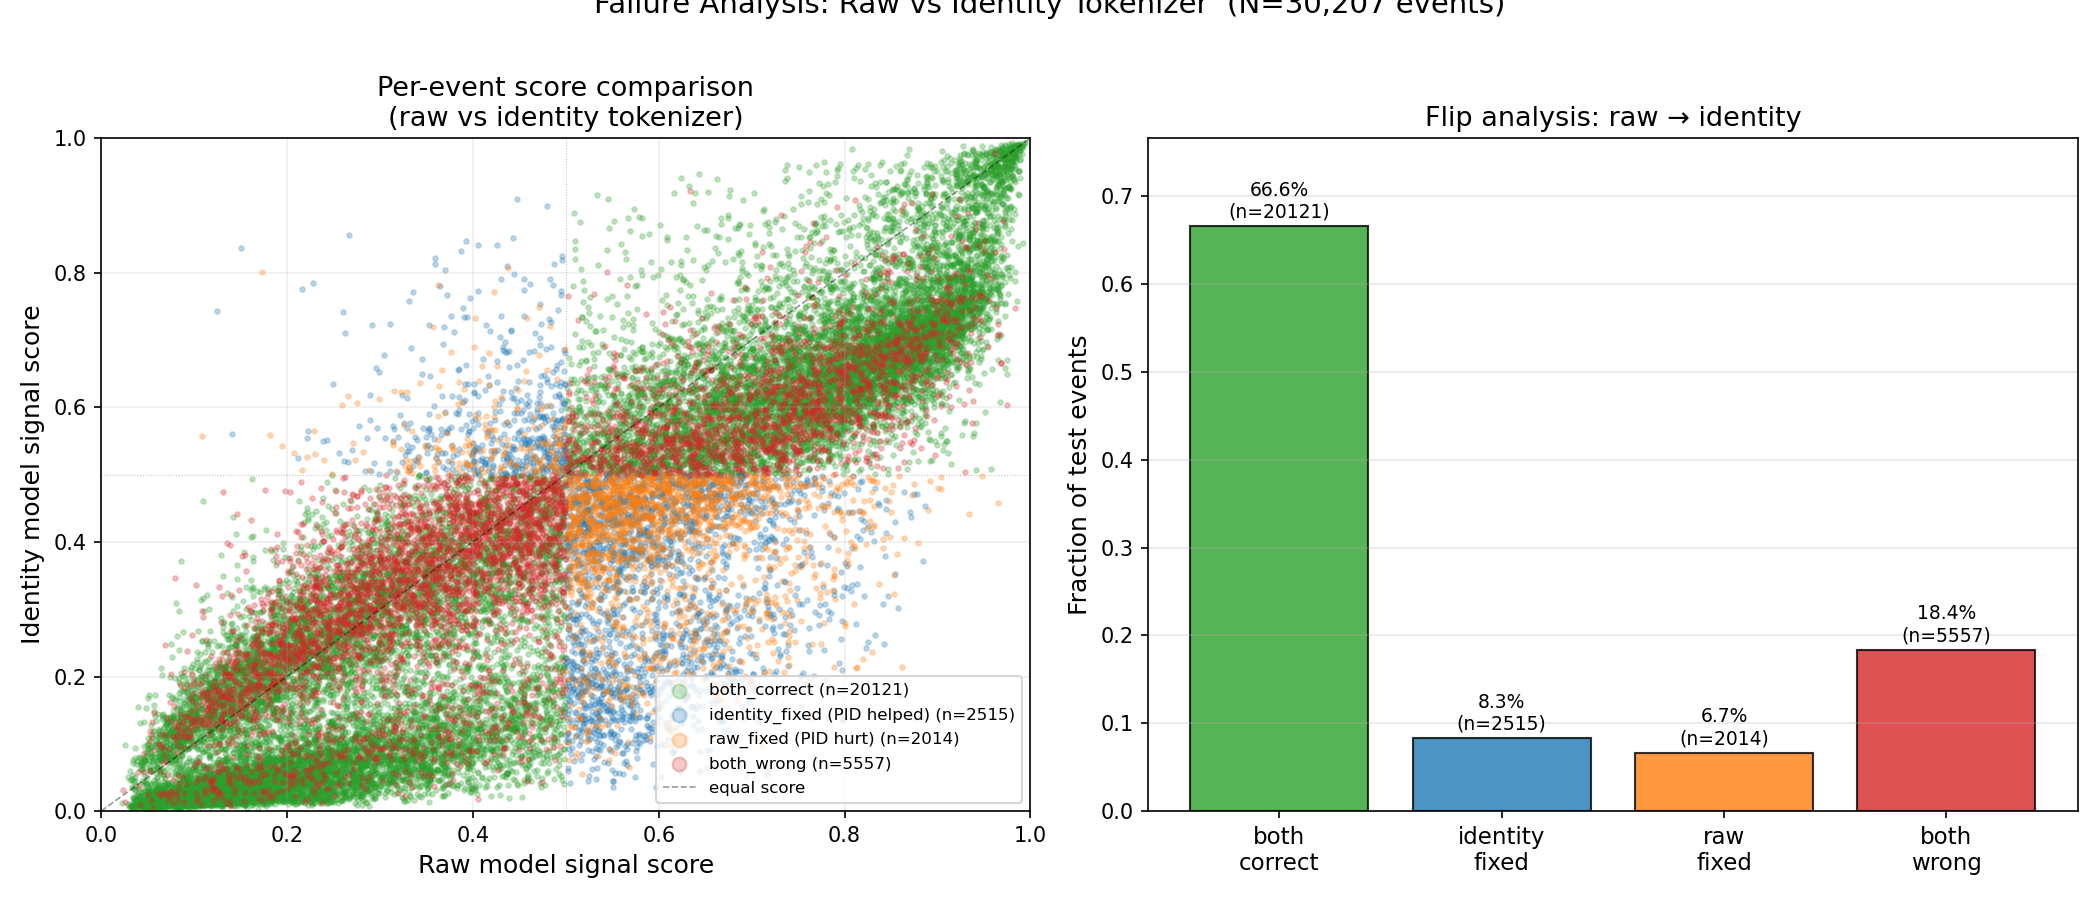
\includegraphics[width=\textwidth]{figures/ch4/figure-failure_analysis_raw_vs_identity.png}
\caption{Failure analysis comparing per-event classifier scores for the
\texttt{raw} (x-axis) and \texttt{identity} (y-axis) tokenizers on the
test set ($N=30{,}207$ events).
\textit{Left:} scatter of per-event signal scores; colours indicate outcome category.
\textit{Right:} fraction of events in each category.
Events above the diagonal benefit from the explicit PID label;
events below are hurt by it.
% NOTE: a follow-up plot breaking down the "identity_fixed" and "raw_fixed"
%   populations by kinematic variables (e.g. jet multiplicity, b-jet pT)
%   would strengthen the interpretability argument. Flag for additional inference.
}
\label{fig:failure-analysis}
\end{figure}

% ============================================================
\section{Feature content and token ordering (Exp.\ 4B)}
\label{sec:exp4b}
% ============================================================

% --- SECTION INTRO NOTE ---
% 1 short paragraph: fix T1=identity, T1-a=one_hot (or learned+dim=16),
%   T1-b=8 (for one_hot). Then ask three independent questions about
%   what information the tokens carry: D01 (energy), D02 (MET), D03 (order).
%   Refer to Table~\ref{tab:exp4b}.

\begin{table}[h]
\centering
\small
\begin{tabular}{lllr}
\toprule
Factor & Axis & Values & $n_\text{configs}$ \\
\midrule
Feature set & D01 & \texttt{[0,1,2,3]} $\cdot$ \texttt{[1,2,3]} & 2 \\
MET included & D02 & \texttt{false} $\cdot$ \texttt{true} & 2 \\
Token order & D03 & \texttt{input\_order} $\cdot$ \texttt{shuffled} & 2 \\
\midrule
\multicolumn{3}{l}{Unique configurations ($2^3$)} & 8 \\
\multicolumn{3}{l}{Seeds per configuration} & 3 \\
\multicolumn{3}{l}{\textbf{Total runs}} & \textbf{24} \\
\bottomrule
\end{tabular}
\caption{Experiment 4B sweep design.
Fixed: T1\,=\,\texttt{identity}, T1-a\,=\,\texttt{one\_hot}, T1-b\,=\,8.
% NOTE: confirm whether Exp 4B was actually run with one_hot or learned.
%   If learned+dim=8, the baseline AUROC will be depressed relative to the
%   best identity configuration. Cross-check against run configs before finalising.
}
\label{tab:exp4b}
\end{table}

% -------------------------------------------------------
\subsection{Energy inclusion (D01)}
\label{sec:exp4b-energy}
% -------------------------------------------------------

% --- NOTE ---
% Numbers: all_features (E,pT,η,φ) = 0.835 vs no_energy (pT,η,φ) = 0.826.
%   Gap = -0.009 AUROC when energy is dropped.
%
% Argument:
%   (1) Physics lens: energy E is not Lorentz-invariant, but it encodes mass
%       information via m² = E² - |p|². For top quark decay products
%       (W bosons, b-jets), the invariant masses of sub-systems are powerful
%       discriminants. Dropping E removes the model's ability to reconstruct
%       these masses implicitly.
%   (2) ML lens: the gap is modest (0.009), suggesting the model partially
%       compensates using the remaining three features. At fixed η, the
%       relationship E ≈ pT·cosh(η) holds for massless particles, so pT and η
%       together recover most of E for light jets and photons. The residual
%       gap reflects the genuinely mass-sensitive component.
%   (3) Practical conclusion: include energy (D01 = [0,1,2,3]) in the baseline.
%
% 2 sentences of argument + figure.

Removing the energy component (D01\,=\,\texttt{[1,2,3]}) reduces mean AUROC
by $0.009$ relative to the full four-vector (D01\,=\,\texttt{[0,1,2,3]},
AUROC\,=\,$0.835$).

\begin{figure}[h]
\centering
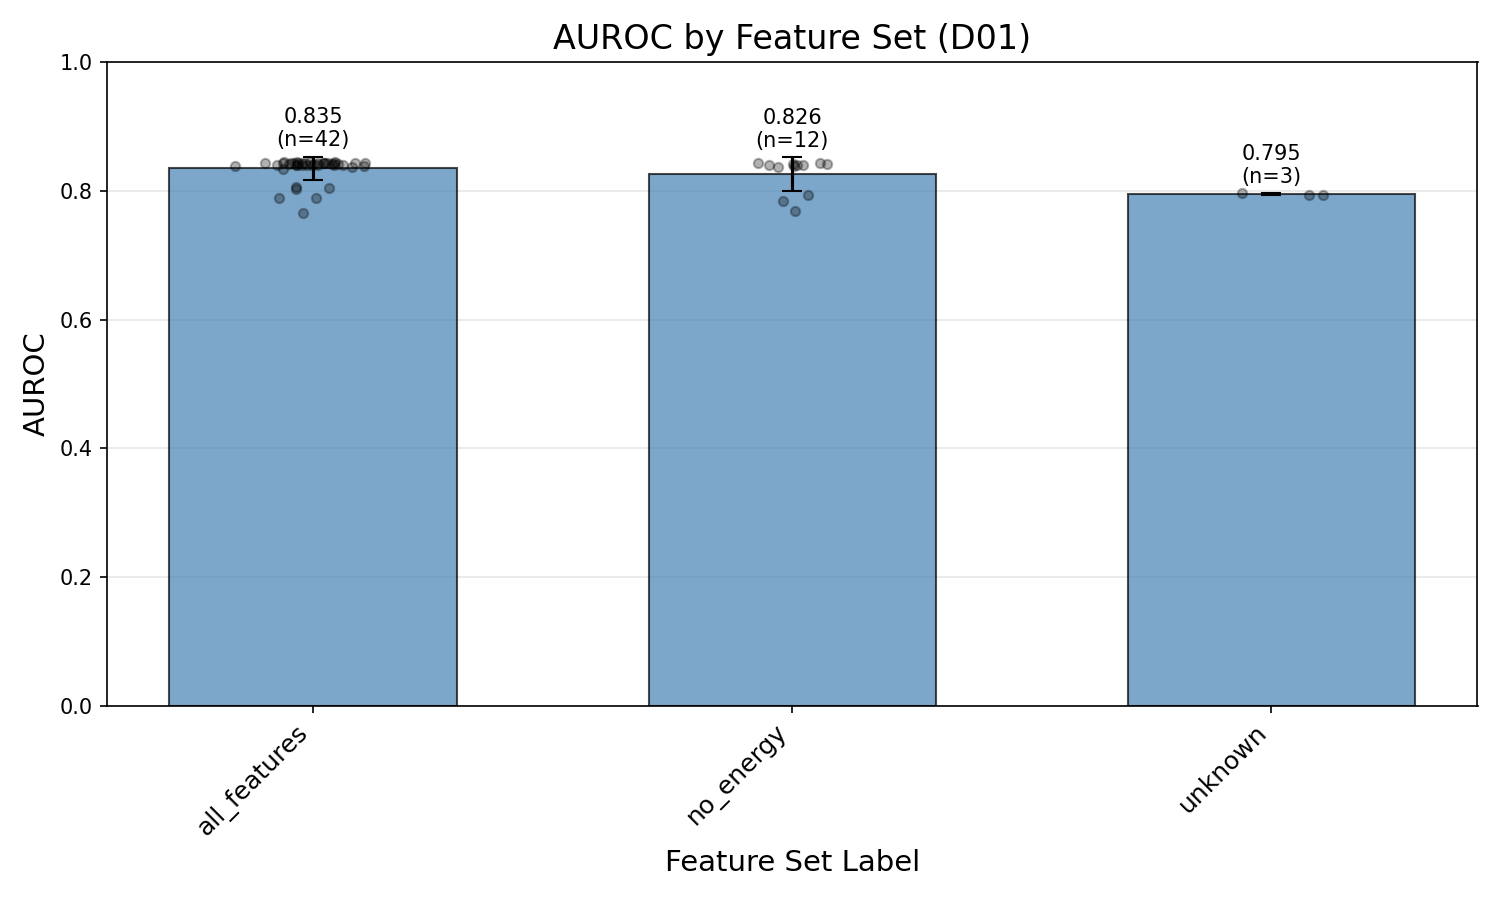
\includegraphics[width=0.65\textwidth]{figures/ch4/figure-auroc_bar_by_features.png}
\caption{Mean test AUROC by feature set (D01).
\texttt{all\_features}: $(E, p_T, \eta, \phi)$;
\texttt{no\_energy}: $(p_T, \eta, \phi)$.
The \texttt{unknown} bar corresponds to the \texttt{binned} tokenizer runs,
where continuous features are not directly accessible, included for completeness.
% NOTE: the "unknown" bar is confusing. Consider either dropping it or
%   relabelling it explicitly as "binned (no continuous features)".
%   Also consider adding a horizontal reference line at raw AUROC = 0.804
%   to contextualise the energy gap.
}
\label{fig:auroc-bar-features}
\end{figure}

% -------------------------------------------------------
\subsection{Missing transverse energy (D02)}
\label{sec:exp4b-met}
% -------------------------------------------------------

% --- NOTE ---
% Numbers: without MET = 0.836, with MET = 0.810. Gap = -0.026.
%   This is a NEGATIVE result: MET HURTS.
%
% This needs honest treatment. Three candidate explanations:
%
%   (A) PE-confusion hypothesis (leading candidate):
%       The sinusoidal positional encoding (E1=sinusoidal, positional_space=model)
%       is active in these runs. Token position carries a signal (as shown
%       by D03 below). MET is appended as an additional token at a fixed
%       position. If attention patterns have learned to associate position
%       with particle type, inserting a MET token at a fixed slot disrupts
%       those patterns for all other tokens.
%
%   (B) Noise injection:
%       MET reconstruction in high-multiplicity events (≥8 jets + leptons)
%       has large experimental resolution. The MET token may carry more
%       noise than signal, particularly for the 4t-vs-bg task where the
%       MET significance varies strongly across background processes.
%
%   (C) Interaction with D03:
%       If the D02=true runs were all run with input_order (D03=false),
%       the MET token appears at a fixed position, compounding hypothesis A.
%       Cross-check: does MET still hurt when D03=shuffled? If the gap
%       disappears under shuffling, hypothesis A is confirmed.
%       [FLAG: this cross-check may require a targeted additional run of
%        ~6 configurations: D02=true × D03=shuffled × 3 seeds.]
%
% Practical conclusion for Ch5+: D02=false. MET is revisited in Ch5
%   where physics-informed attention biases (B1-G1=met_direction) provide
%   a more principled way to inject MET information.
%
% Write ~2 paragraphs: (1) state the result; (2) discuss the explanation
%   candidates. Keep the D03 cross-check as a parenthetical or footnote.

Contrary to the expectation that missing transverse energy provides
additional signal from the neutrino system,
including MET as a token (D02\,=\,\texttt{true}) reduces mean AUROC
by $0.026$ relative to the MET-free baseline ($0.836$ vs $0.810$).

\begin{figure}[h]
\centering
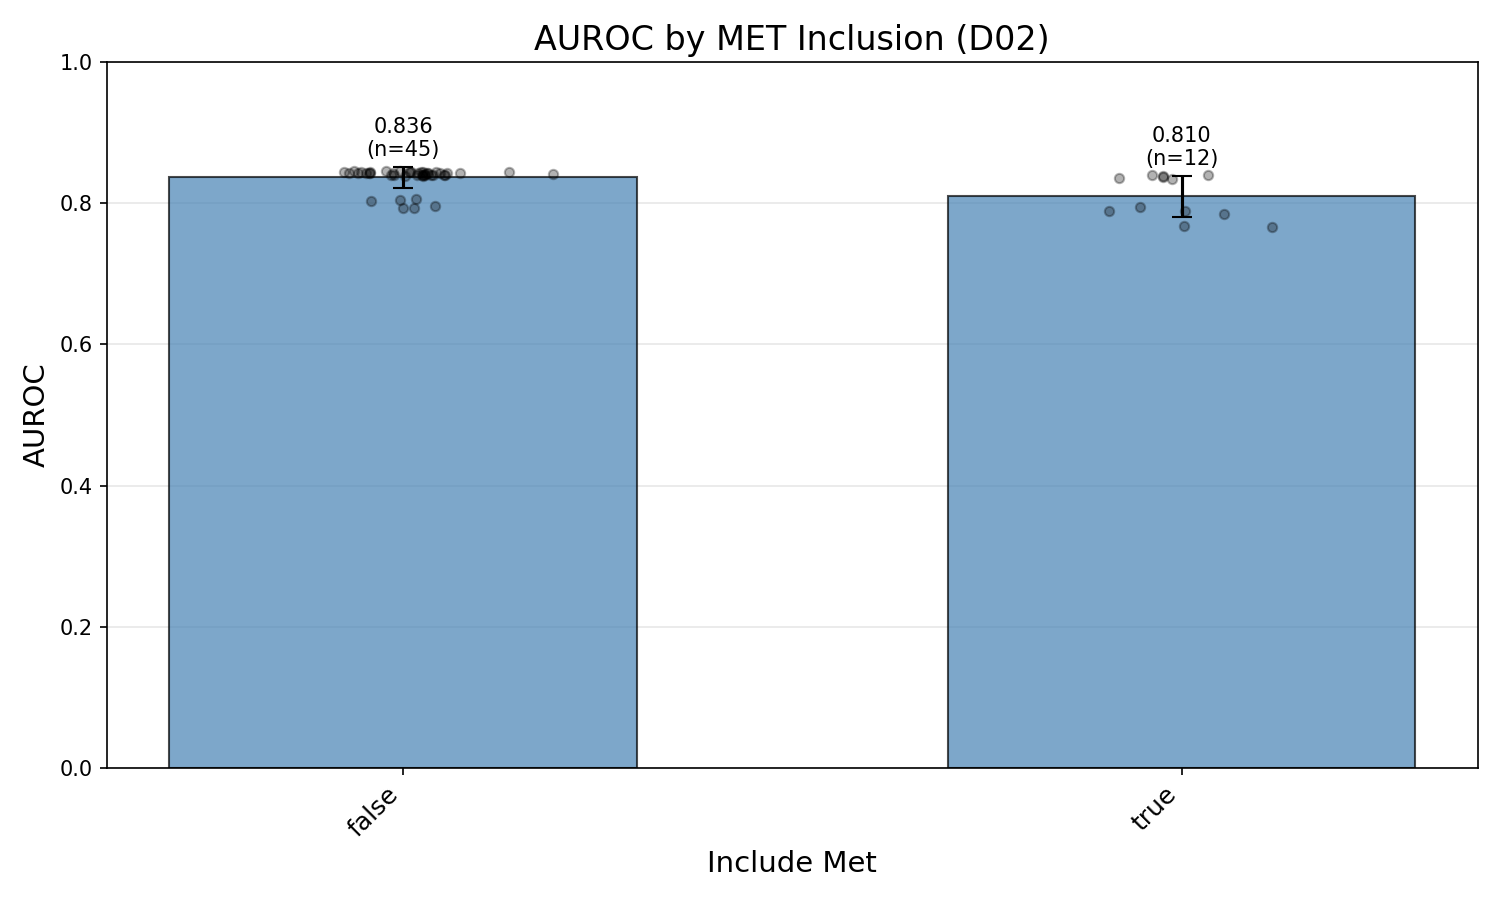
\includegraphics[width=0.65\textwidth]{figures/ch4/figure-auroc_bar_by_met.png}
\caption{Mean test AUROC by MET inclusion (D02).
Including MET as a token degrades performance by $0.026$ AUROC on the
4t-vs-background task.
% NOTE: if the D03 cross-check runs are available (D02=true × D03=shuffled),
%   add a second grouped bar showing MET effect separately for ordered and
%   shuffled conditions. This is the key diagnostic for the PE-confusion hypothesis.
}
\label{fig:auroc-bar-met}
\end{figure}

% [NEED] Figure: MET effect stratified by D03 ordering condition
%   (to test PE-confusion hypothesis). Requires ~6 additional runs.
% \begin{figure}[h]
% \centering
% \includegraphics[width=0.65\textwidth]{figures/ch4/figure-auroc_met_by_ordering.png}
% \caption{[PLACEHOLDER] Mean test AUROC as a function of MET inclusion (D02),
%   shown separately for ordered (D03=input\_order) and shuffled (D03=shuffled)
%   token sequences. If the MET penalty disappears under shuffling, the
%   PE-confusion hypothesis is confirmed.}
% \label{fig:auroc-met-by-ordering}
% \end{figure}

% -------------------------------------------------------
\subsection{Token ordering as a permutation-invariance diagnostic (D03)}
\label{sec:exp4b-order}
% -------------------------------------------------------

% --- NOTE ---
% Numbers: input_order = 0.840, shuffled = 0.811. Gap = -0.029.
%
% This is the second surprise. Self-attention is permutation-equivariant
%   by construction (no positional encoding → truly order-invariant).
%   But all these runs use E1=sinusoidal with positional_space=model.
%   Sinusoidal PE injects an ordering signal. If the input ordering has
%   any physical structure (e.g., particles ordered by reconstruction
%   algorithm output, or by pT descending), the PE effectively becomes
%   a pT-proxy or type-proxy.
%
% Consequence: the -0.029 gap does NOT mean the attention mechanism is
%   exploiting ordering. It means the sinusoidal PE is exploiting ordering.
%   True permutation invariance requires E1=none.
%
% This result does two things for the thesis:
%   (1) It closes the chapter with a concrete negative finding that
%       motivates the positional encoding chapter (if one exists) or
%       at minimum serves as a caveat for all PE=sinusoidal results.
%   (2) It means that for any future chapter, D03=input_order is the
%       correct default (not shuffled), since the model uses the ordering.
%       But the physics meaning of that ordering should be checked.
%
% [FLAG: check what ordering the reconstruction software produces.
%   If it is pT-descending, the PE is effectively encoding pT rank,
%   which is a legitimate (if implicit) physics feature. If it is
%   arbitrary, the PE may be encoding noise.]
%
% Write ~2 paragraphs: (1) state the result and why it is surprising;
%   (2) explain the PE mechanism and what it implies for subsequent chapters.

Shuffling the token sequence (D03\,=\,\texttt{shuffled}) reduces mean AUROC
from $0.840$ to $0.811$ ($-0.029$),
despite self-attention being permutation-equivariant by construction.

\begin{figure}[h]
\centering
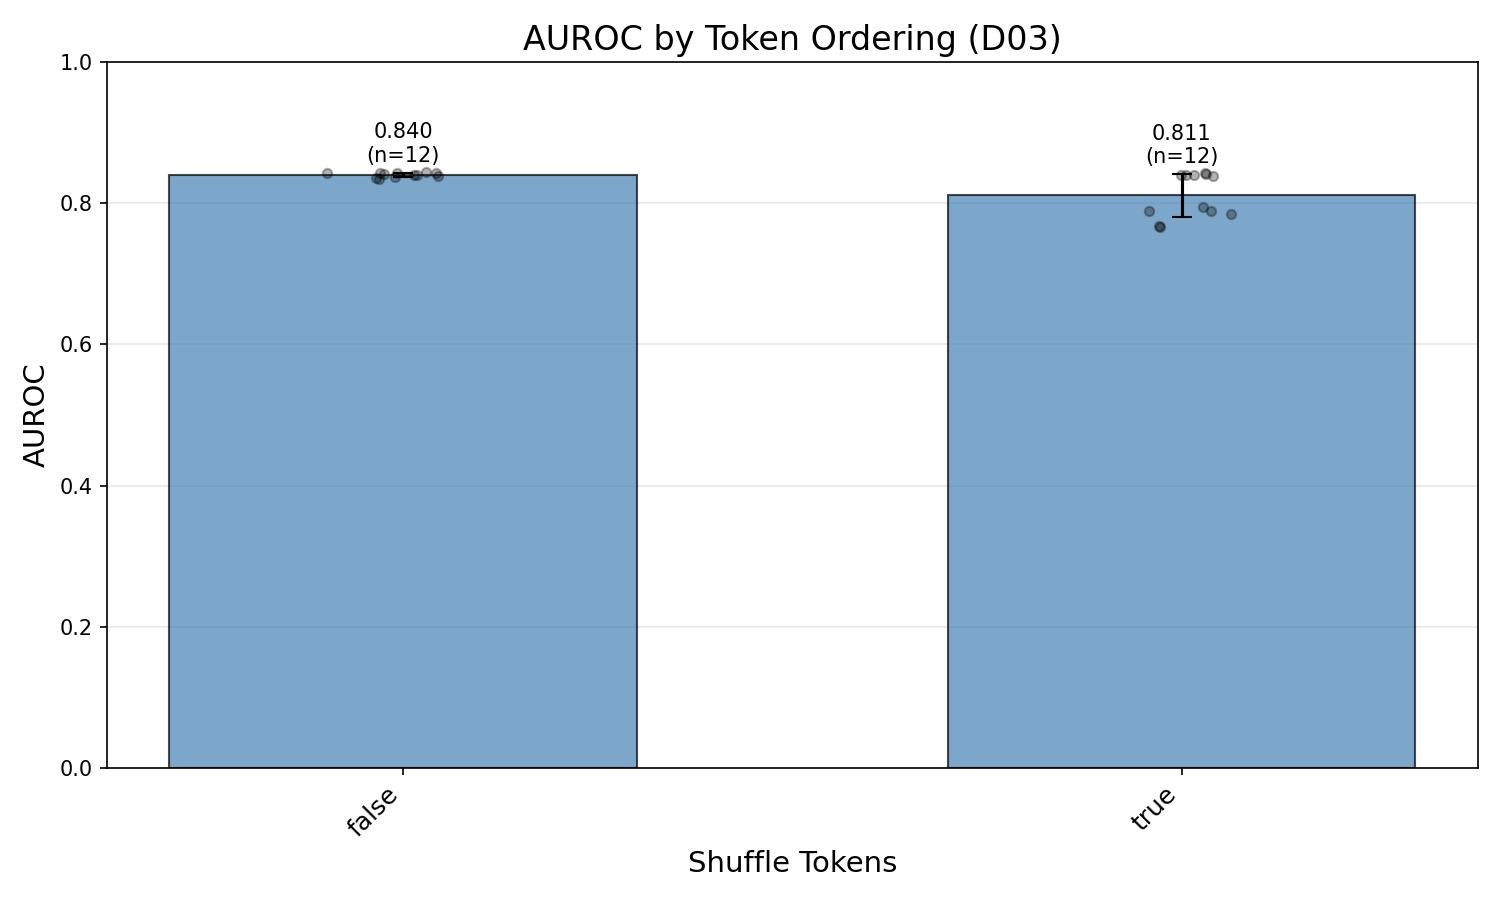
\includegraphics[width=0.65\textwidth]{figures/ch4/figure-auroc_bar_by_shuffle.png}
\caption{Mean test AUROC by token ordering (D03).
The performance gap under shuffling ($-0.029$) indicates that the sinusoidal
positional encoding (E1\,=\,\texttt{sinusoidal}) is exploiting the input
ordering of the particle sequence.
True permutation invariance would require E1\,=\,\texttt{none}.
% NOTE: if the report generates a val_auroc_by_shuffle training curve,
%   include it here to show whether shuffled models converge differently
%   or simply plateau lower.
}
\label{fig:auroc-bar-shuffle}
\end{figure}

% [NEED] Figure: training curves D03=ordered vs shuffled
%   (does shuffled model converge differently or just plateau lower?)
% \begin{figure}[h]
% \centering
% 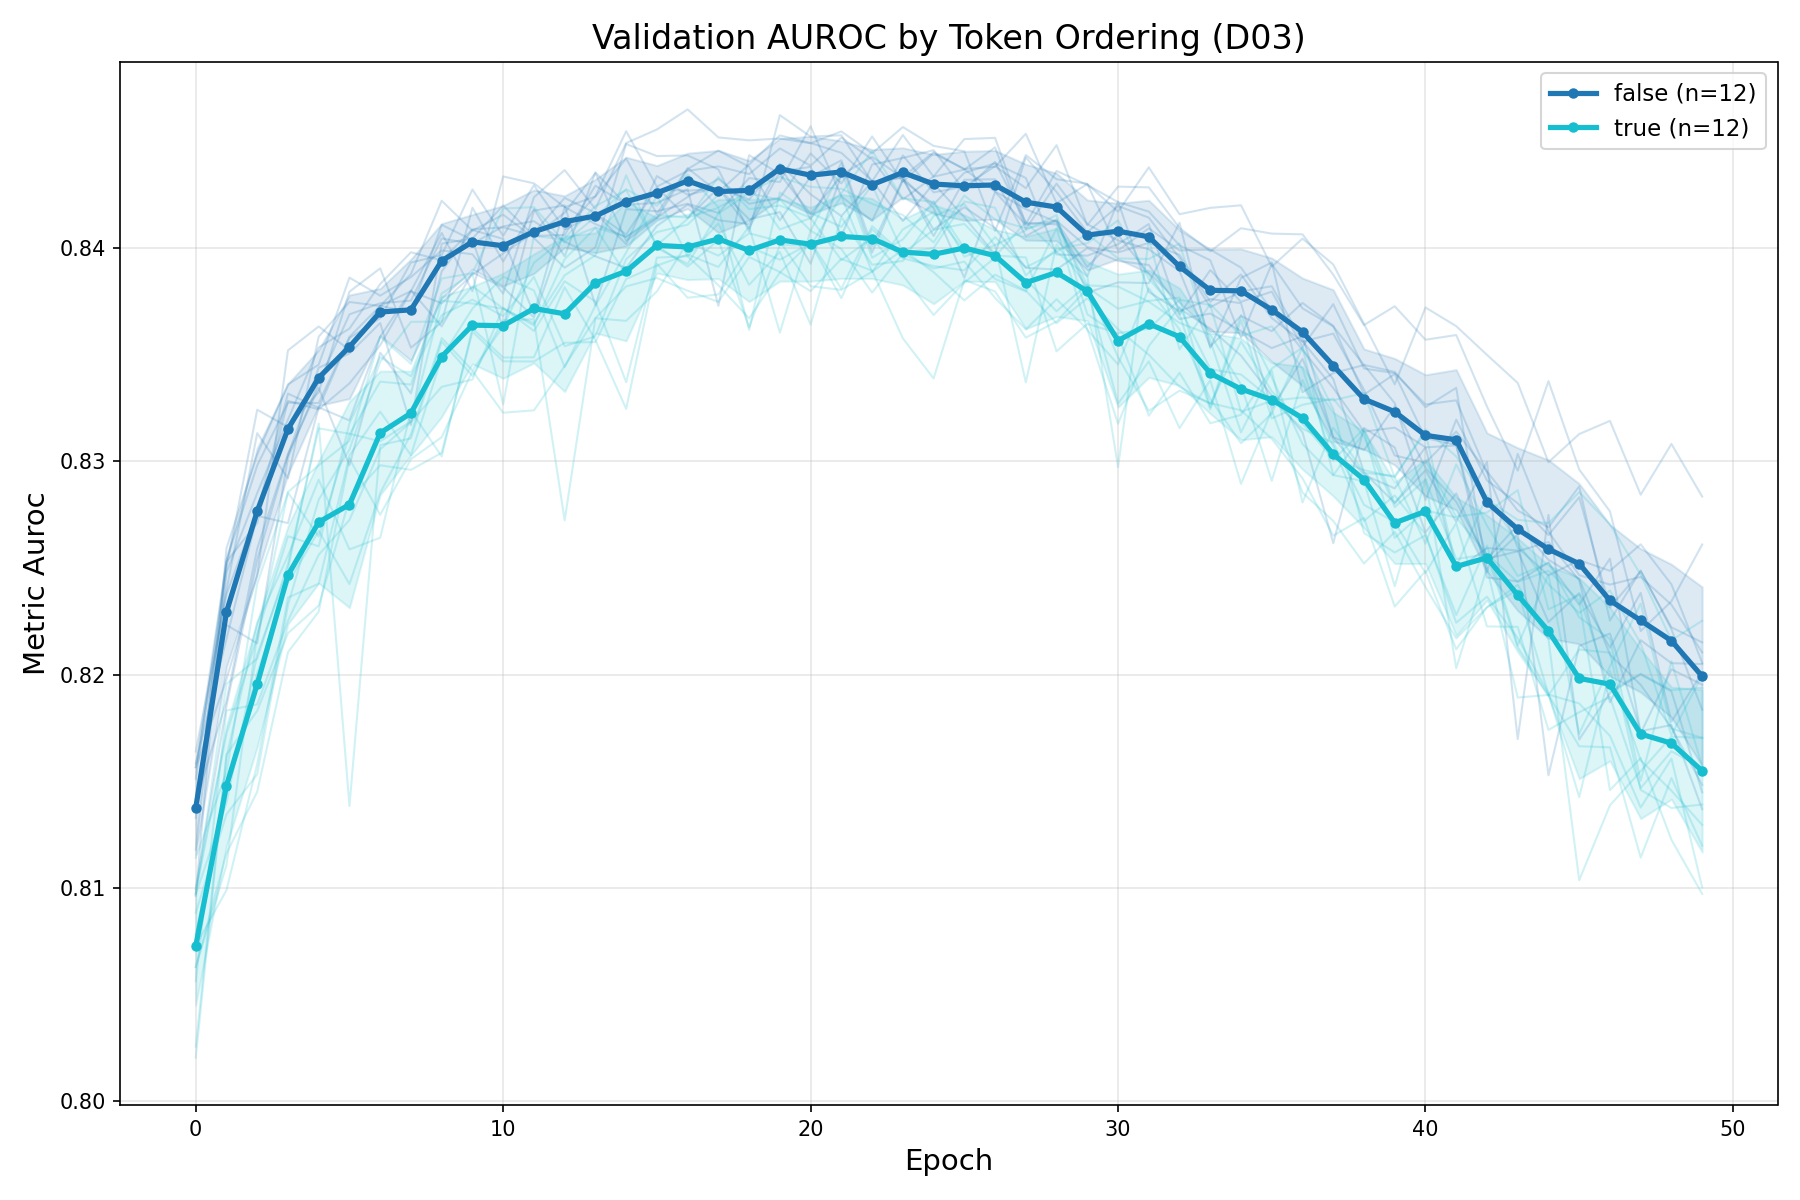
\includegraphics[width=0.65\textwidth]{figures/ch4/figure-val_auroc_by_shuffle.png}
% \caption{[PLACEHOLDER] Validation AUROC training curves for ordered vs
%   shuffled token sequences.}
% \label{fig:val-auroc-shuffle}
% \end{figure}

% [NEED] Figure: AUROC as function of D03, stratified by E1 (PE type),
%   specifically comparing E1=sinusoidal vs E1=none.
%   This would confirm that the shuffle penalty disappears when PE=none.
%   Requires ~6 additional runs: E1=none × D03=shuffled/ordered × 3 seeds.
%   Medium priority — useful for the PE chapter but also here.
% \begin{figure}[h]
% \centering
% \includegraphics[width=0.65\textwidth]{figures/ch4/figure-auroc_shuffle_by_pe.png}
% \caption{[PLACEHOLDER] Shuffle penalty as a function of positional encoding type.
%   E1=none should show no ordering effect; E1=sinusoidal should reproduce
%   the $-0.029$ gap observed here.}
% \label{fig:auroc-shuffle-by-pe}
% \end{figure}

% ============================================================
\section{Summary and chapter baseline}
\label{sec:ch4-summary}
% ============================================================

% --- NOTE ---
% Short section (~1 paragraph + table). State the three main findings:
%   (1) PID is load-bearing: the transformer cannot recover particle
%       identity from kinematics alone at this capacity. +0.031 AUROC.
%   (2) How PID is encoded matters only at low embedding dimension:
%       at dim≥16, all encoding modes are equivalent. one_hot at dim=8
%       is the parameter-efficient choice.
%   (3) Two counterintuitive negatives: MET hurts (-0.026) and shuffling
%       hurts (-0.029). Both implicate the sinusoidal positional encoding,
%       which is exploiting input ordering and may be disrupted by an
%       additional fixed-position MET token.
%
% Then: Table~\ref{tab:ch4-baseline} stating the chosen values for each
%   axis, with a one-line justification for each.
%
% Final sentence: these choices constitute the Ch5 baseline. Any subsequent
%   chapter that changes one of these axes re-runs the relevant comparison
%   on top of this configuration.

This chapter establishes six axis choices that propagate as the fixed baseline
into all subsequent chapters.
Three main conclusions motivate these choices.

First, an explicit particle-type label is necessary:
the \texttt{identity} tokenizer outperforms kinematics-only \texttt{raw}
by $+0.031$ AUROC,
and the failure analysis shows that this gap is concentrated in events
where particle type, not kinematics, carries the discriminating signal.
The \texttt{binned} tokenizer, which discards continuous features entirely,
is the weakest of the three families.

Second, the choice of PID encoding mode (T1-a) is largely irrelevant
provided the embedding dimension is at least 16 for the \texttt{learned} mode.
The \texttt{one\_hot} encoding at dimension 8 is robust and parameter-efficient,
making it the preferred baseline.

Third, two results indicate that the sinusoidal positional encoding (E1)
is a confounding variable in this chapter.
MET inclusion degrades performance ($-0.026$), most likely because the MET token
disrupts the attention patterns that the model has learned to associate with
input token position.
Similarly, shuffling the token sequence degrades performance ($-0.029$),
demonstrating that the model exploits the input ordering via the positional encoding
rather than being genuinely permutation-invariant.
Both effects point to the positional encoding as an implicit inductive bias
whose interaction with physics-motivated design choices warrants further study.

\begin{table}[h]
\centering
\small
\begin{tabular}{llll}
\toprule
Axis & Config key & Chosen value & Justification \\
\midrule
T1   & \texttt{tokenizer.name}     & \texttt{identity}    & $+0.031$ over \texttt{raw} \\
T1-a & \texttt{tokenizer.pid\_mode} & \texttt{one\_hot}    & robust at dim=8; no learning needed \\
T1-b & \texttt{tokenizer.id\_embed\_dim} & 8           & sufficient for \texttt{one\_hot} \\
D01  & \texttt{data.cont\_features} & \texttt{[0,1,2,3]}  & $+0.009$ from energy inclusion \\
D02  & \texttt{include\_met}        & \texttt{false}       & MET token degrades AUROC \\
D03  & \texttt{shuffle\_tokens}     & \texttt{false}       & model exploits input ordering \\
\bottomrule
\end{tabular}
\caption{Chapter 4 baseline configuration carried forward to all subsequent chapters.
% NOTE: T1-a choice may need revisiting if the planned cross-task (4t-vs-ttH)
%   results show a different ranking. Confirm before freezing.
}
\label{tab:ch4-baseline}
\end{table}

% [NEED] Cross-task validation subsection (or box):
%   Re-run T1 and D02 comparisons on the 4t-vs-ttH task.
%   Expected: T1 finding replicates (identity still best).
%   D02: on 4t-vs-ttH both signal and background have semi-leptonic tops,
%   so MET provides even less discriminating power, and the negative
%   result should be as strong or stronger.
%   6--12 additional runs. Include as a subsection if results are available;
%   otherwise move to an appendix or footnote.
%
% \subsection{Cross-task validation on $tttt$ vs $ttH$ (optional)}
% \label{sec:ch4-crosstask}
% [PLACEHOLDER: 1 figure, ~1 paragraph]

\chapter{Physics-Informed Attention Biases}
\label{ch:biases}

Standard self-attention assigns relevance to token pairs through learned
query--key inner products, making no assumption about the physical
relationships among the particles those tokens represent. In a
four-tops-versus-background event, however, pairs of particles that share
a decay vertex, are separated by a small angle, or interact through a
specific Standard Model (SM) coupling are physically more related than
arbitrary token pairs. This chapter investigates whether encoding such
structure as additive biases on the attention logits improves
classification performance, and what the learned bias weights reveal about
how the model organises particle interactions.

Four bias families are available in the workbench. The
\textit{Lorentz-scalar bias}~(\wandbaxis{B1-L}) maps pairwise kinematic
invariants to attention scores through a small sub-network. The
\textit{type-pair table}~(\wandbaxis{B1-T}) is a learnable
$N_\mathrm{type}\times N_\mathrm{type}$ matrix that assigns a baseline
attention score to every ordered pair of particle types, optionally
initialised from SM coupling constants. The \textit{SM interaction
prior}~(\wandbaxis{B1-S}) encodes SM coupling topology as a fixed or
learned additive bias parametrised by coupling constants. The
\textit{global-conditioned bias}~(\wandbaxis{B1-G}) modulates attention
using a global event-level feature such as missing transverse energy (MET)
direction. All families share a zero-initialised scalar gate, so adding
any bias leaves the transformer output unchanged at initialisation;
the gate must be driven away from zero for the bias to have any effect.
All experiments in this chapter hold \wandbaxis{D02}~(\texttt{include\_met})
at \texttt{true}: MET is always present, as motivated by the Ch.\,4
findings, and is required for the B1-G family to operate.

The primary lens throughout this chapter is \textit{interpretability}.
Performance differences between bias configurations are expected to be
small, and the main scientific contribution is understanding what structure
the model learns to place on particle-pair relationships when given
physics-motivated inductive biases. Section~\ref{sec:5a} establishes the
performance envelope across all four families and examines attention maps
as the central interpretability tool. Sections~\ref{sec:5b}
through~\ref{sec:5d} drill into the internal design choices of each
family, and Section~\ref{sec:5_synthesis} draws the chapter together.


% ──────────────────────────────────────────────
\section{Bias family comparison (Exp.\ 5A)}
\label{sec:5a}

\subsection{Experimental design}

Experiment 5A asks whether any of the four bias families, applied
individually or in full combination, measurably improves classification
accuracy relative to an unbiased transformer baseline, and whether the
full stack is super-additive. Eighteen runs cover six bias configurations
at three seeds each: \texttt{none} (unbiased baseline),
\texttt{lorentz\_scalar}, \texttt{typepair\_kinematic},
\texttt{sm\_interaction}, \texttt{global\_conditioned}, and all four
combined. All other axes are held at the chapter baseline: embedding
dimension 128 (\wandbaxis{H01}), depth 3 (\wandbaxis{H02}), 4 heads
(\wandbaxis{H03}), MLP dimension 256 (\wandbaxis{H04}), tokeniser
\texttt{identity} (\wandbaxis{T1}), positional encoding
\texttt{sinusoidal} (\wandbaxis{E1}), and PID embedding mode
\texttt{learned} with dimension 8.

\begin{table}[h]
\centering\small
\begin{tabular}{llr}
\toprule
Axis & Values & Levels \\
\midrule
\wandbaxis{B1} — Bias selector & \texttt{none} & 6 \\
 & \texttt{lorentz\_scalar} & \\
 & \texttt{typepair\_kinematic} & \\
 & \texttt{sm\_interaction} & \\
 & \texttt{global\_conditioned} & \\
 & \texttt{lorentz+typepair+sm+global} & \\
Seeds (\wandbaxis{R5}) & 42, 123, 314 & 3 \\
\midrule
Total & & \textbf{18} \\
\bottomrule
\end{tabular}
\caption{Exp.\ 5A design. All other axes at chapter baseline:
\wandbaxis{T1}~=~\texttt{identity}, \wandbaxis{D02}~=~\texttt{true},
\wandbaxis{E1}~=~\texttt{sinusoidal}, dim 128, depth 3, 4 heads.}
\label{tab:5a_design}
\end{table}

\subsection{Performance results}

Table~\ref{tab:5a_auroc} reports seed-mean test AUROC and per-cell seed
standard deviation ($n=3$) for each configuration. The \texttt{none}
baseline achieves $0.84125 \pm 0.00068$.

\begin{table}[h]
\centering\small
\begin{tabular}{lrrl}
\toprule
B1 configuration & Mean AUROC & Seed std & $\Delta$ vs baseline \\
\midrule
\texttt{none} (baseline)                 & 0.84125 & 0.00068 & --- \\
\texttt{lorentz\_scalar}                 & 0.84156 & 0.00029 & $+0.00031$ \\
\texttt{typepair\_kinematic}             & 0.84155 & 0.00080 & $+0.00030$ \\
\texttt{sm\_interaction}                 & 0.84080 & 0.00136 & $-0.00045$ \\
\texttt{global\_conditioned}             & 0.84170 & 0.00091 & $+0.00045$ \\
\texttt{lorentz+typepair+sm+global}      & 0.83937 & 0.00090 & $-0.00188$ \\
\bottomrule
\end{tabular}
\caption{Exp.\ 5A seed-mean test AUROC ($n = 3$ seeds per cell). Per-cell
seed standard deviation is indicative only; inter-cell range ($\approx 0.002$)
is comparable to seed variance.}
\label{tab:5a_auroc}
\end{table}

\begin{figure}[h]
\centering
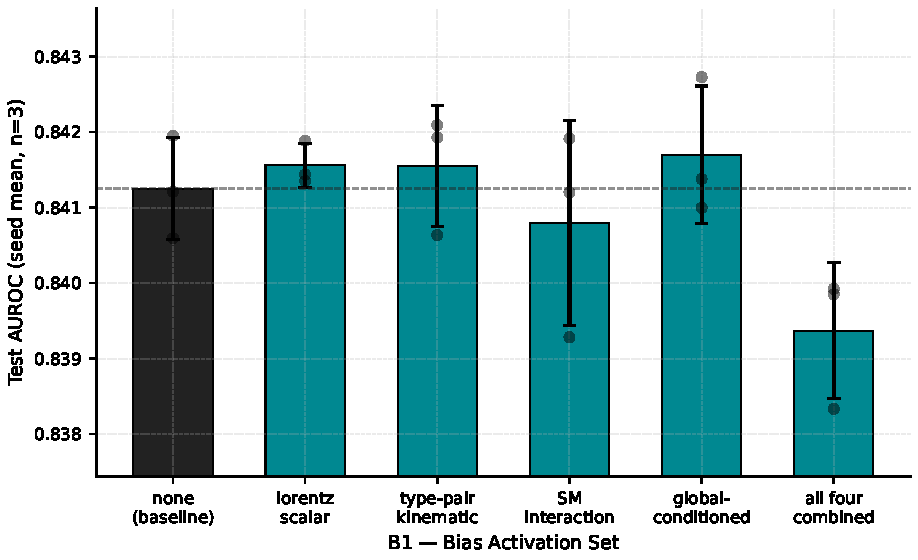
\includegraphics[width=\textwidth]{figures/ch5/figure-auroc_bar_by_bias_family}
\caption{Exp.\ 5A seed-mean test AUROC for all six \wandbaxis{B1}
configurations, with per-seed spread. Dashed line marks the \texttt{none}
baseline mean.}
\label{fig:5a_auroc_bar}
\end{figure}

Three observations follow directly from these results. First, no single
bias family moves the seed-mean AUROC by more than approximately one
inter-seed standard deviation away from the \texttt{none} baseline.
The three families that nominally improve accuracy (\texttt{lorentz\_scalar},
\texttt{typepair\_kinematic}, \texttt{global\_conditioned}) each gain at
most $+0.00045$ AUROC, which is smaller than the per-cell seed standard
deviation of the baseline itself. Second, \texttt{sm\_interaction} sits
$-0.00045$ below baseline, within one seed standard deviation. Third,
the full-combination cell is the only configuration whose mean (0.83937)
sits visibly below the baseline, at a deficit of approximately 0.002
AUROC. This result is consistent with mild optimisation interference when
multiple bias signals compete simultaneously for the same attention logit,
though it cannot be cleanly attributed to any single component without
further ablation.

The AUROC metric alone therefore does not reveal a meaningful benefit from
physics-informed attention biases at this model scale and seed budget. The
more informative question is whether the biases restructure attention
towards physically motivated patterns even when the classification boundary
shifts only modestly. The attention map analysis in
Section~\ref{sec:5a_attention_maps} addresses this.

\subsection{Attention structure: none versus full combination}
\label{sec:5a_attention_maps}

Attention weights are extracted at inference time by forwarding 2000
validation events through each model with the \texttt{capture\_attention}
flag enabled, then averaging over all heads, all layers, and all three
seeds. The physical token sub-block (18 particle tokens, positions 1--18
in the 21-token sequence; MET and MET-$\phi$ excluded) is projected onto a
$7\times 7$ type-pair grid by averaging attention from tokens of type $i$
to tokens of type $j$ for each ordered pair $(i, j)$ across events. The
seven physical types are: jet (1), b-jet (2), $e^+$ (3), $e^-$ (4),
$\mu^+$ (5), $\mu^-$ (6), photon (7).

\begin{figure}[h]
\centering
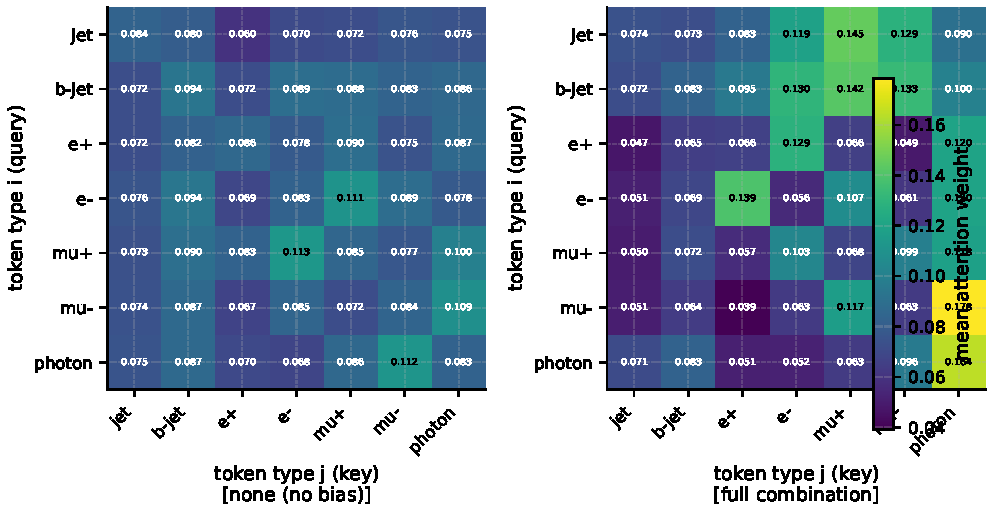
\includegraphics[width=\textwidth]{figures/ch5/figure-attn_typepair_mean_none_vs_full}
\caption{Type-pair mean attention weights for the \texttt{none} baseline
(left) and full-combination model (right), averaged over all heads, layers,
seeds, and 2000 validation events. Particle types: 1~=~jet, 2~=~b-jet,
3~=~$e^+$, 4~=~$e^-$, 5~=~$\mu^+$, 6~=~$\mu^-$, 7~=~photon. Pad tokens
excluded.}
\label{fig:5a_attn_mean}
\end{figure}

In the \texttt{none} baseline, type-pair attention weights occupy a
near-uniform range of 0.059--0.113. No pair dominates: the largest cell
($\mu^+ \to e^-$: 0.113) and the smallest (inferred from the stated range)
differ by only 0.054 units. The distribution is consistent with a model
that has learned to aggregate broad context without privileging specific
particle-type relationships.

The full-combination model produces a qualitatively different pattern.
Table~\ref{tab:5a_attn} lists the most strongly elevated and depressed
type-pair cells. The attention range widens to 0.039--0.178, a factor of
approximately $2.6$ relative to the baseline range of 0.054. Critically,
the elevated cells correspond to physically motivated interactions.

\begin{table}[h]
\centering\small
\begin{tabular}{llrl}
\toprule
Pair $(i \to j)$ & Mean attention & Physics interpretation \\
\midrule
$\mu^- \to \gamma$   & 0.178 & Lepton--photon (FSR / radiative return) \\
$\text{jet} \to \mu^+$  & 0.145 & Jet-embedded muon (semi-leptonic $b$-decay) \\
$\gamma \to \gamma$  & 0.164 & Photon self-attention (cluster isolation) \\
$b\text{-jet} \to \mu^+$ & 0.142 & Direct $b \to \mu$ semi-leptonic \\
$e^- \to e^+$        & 0.139 & Opposite-sign lepton pair ($Z$/$W$ decay) \\
$b\text{-jet} \to e^-$ & 0.130 & Semi-leptonic $b \to e$ \\
$e^+ \to e^-$        & 0.129 & Opposite-sign lepton pair \\
$\text{jet} \to \mu^-$ & 0.129 & Jet-embedded muon \\
$b\text{-jet} \to \mu^-$ & 0.133 & Semi-leptonic $b$-decay \\
\midrule
$\mu^- \to e^+$      & 0.039 & Same-charge mixed lepton (suppressed) \\
$e^+ \to \mu^-$      & 0.049 & Same-charge mixed lepton (suppressed) \\
\bottomrule
\end{tabular}
\caption{Selected type-pair mean attention weights under the full-combination
model (Exp.\ 5A), averaged over all heads, layers, seeds, and 2000
validation events. Pairs with mean attention $\geq 0.13$ are elevated;
pairs $\leq 0.05$ are depressed.}
\label{tab:5a_attn}
\end{table}

The pattern is interpretable in HEP terms. Lepton--photon pairs
($\mu^- \to \gamma$: 0.178) are associated with final-state radiation or
radiative $W/Z$ decays. Photon self-attention (0.164) reflects the
importance of photon isolation and cluster-shape information. The
$b$-jet-to-muon cells (0.142, 0.133) directly encode the semi-leptonic
$b$-decay topology relevant to top-quark reconstruction, where a $b$ quark
decays to a charm quark and a lepton. Opposite-sign lepton pairs
($e^- \to e^+$: 0.139, $e^+ \to e^-$: 0.129) are consistent with $Z$- or
$W$-boson leptonic decays in the multi-top system. By contrast, same-charge
mixed-lepton pairs ($\mu^- \to e^+$: 0.039) are strongly suppressed, as
expected for pairs that share no direct SM vertex in the $t\bar{t}t\bar{t}$
decay chain.

These results constitute the primary interpretability finding of the
chapter: the physics-informed biases do not substantially improve
classification accuracy on this dataset at this model scale, but they do
restructure the model's attention towards physically motivated particle-type
relationships. The model, when given structured priors through the bias
families, converges to an attention pattern that is broadly consistent with
HEP domain knowledge, even though the AUROC improvement is within seed
noise.

\begin{figure}[h]
\centering
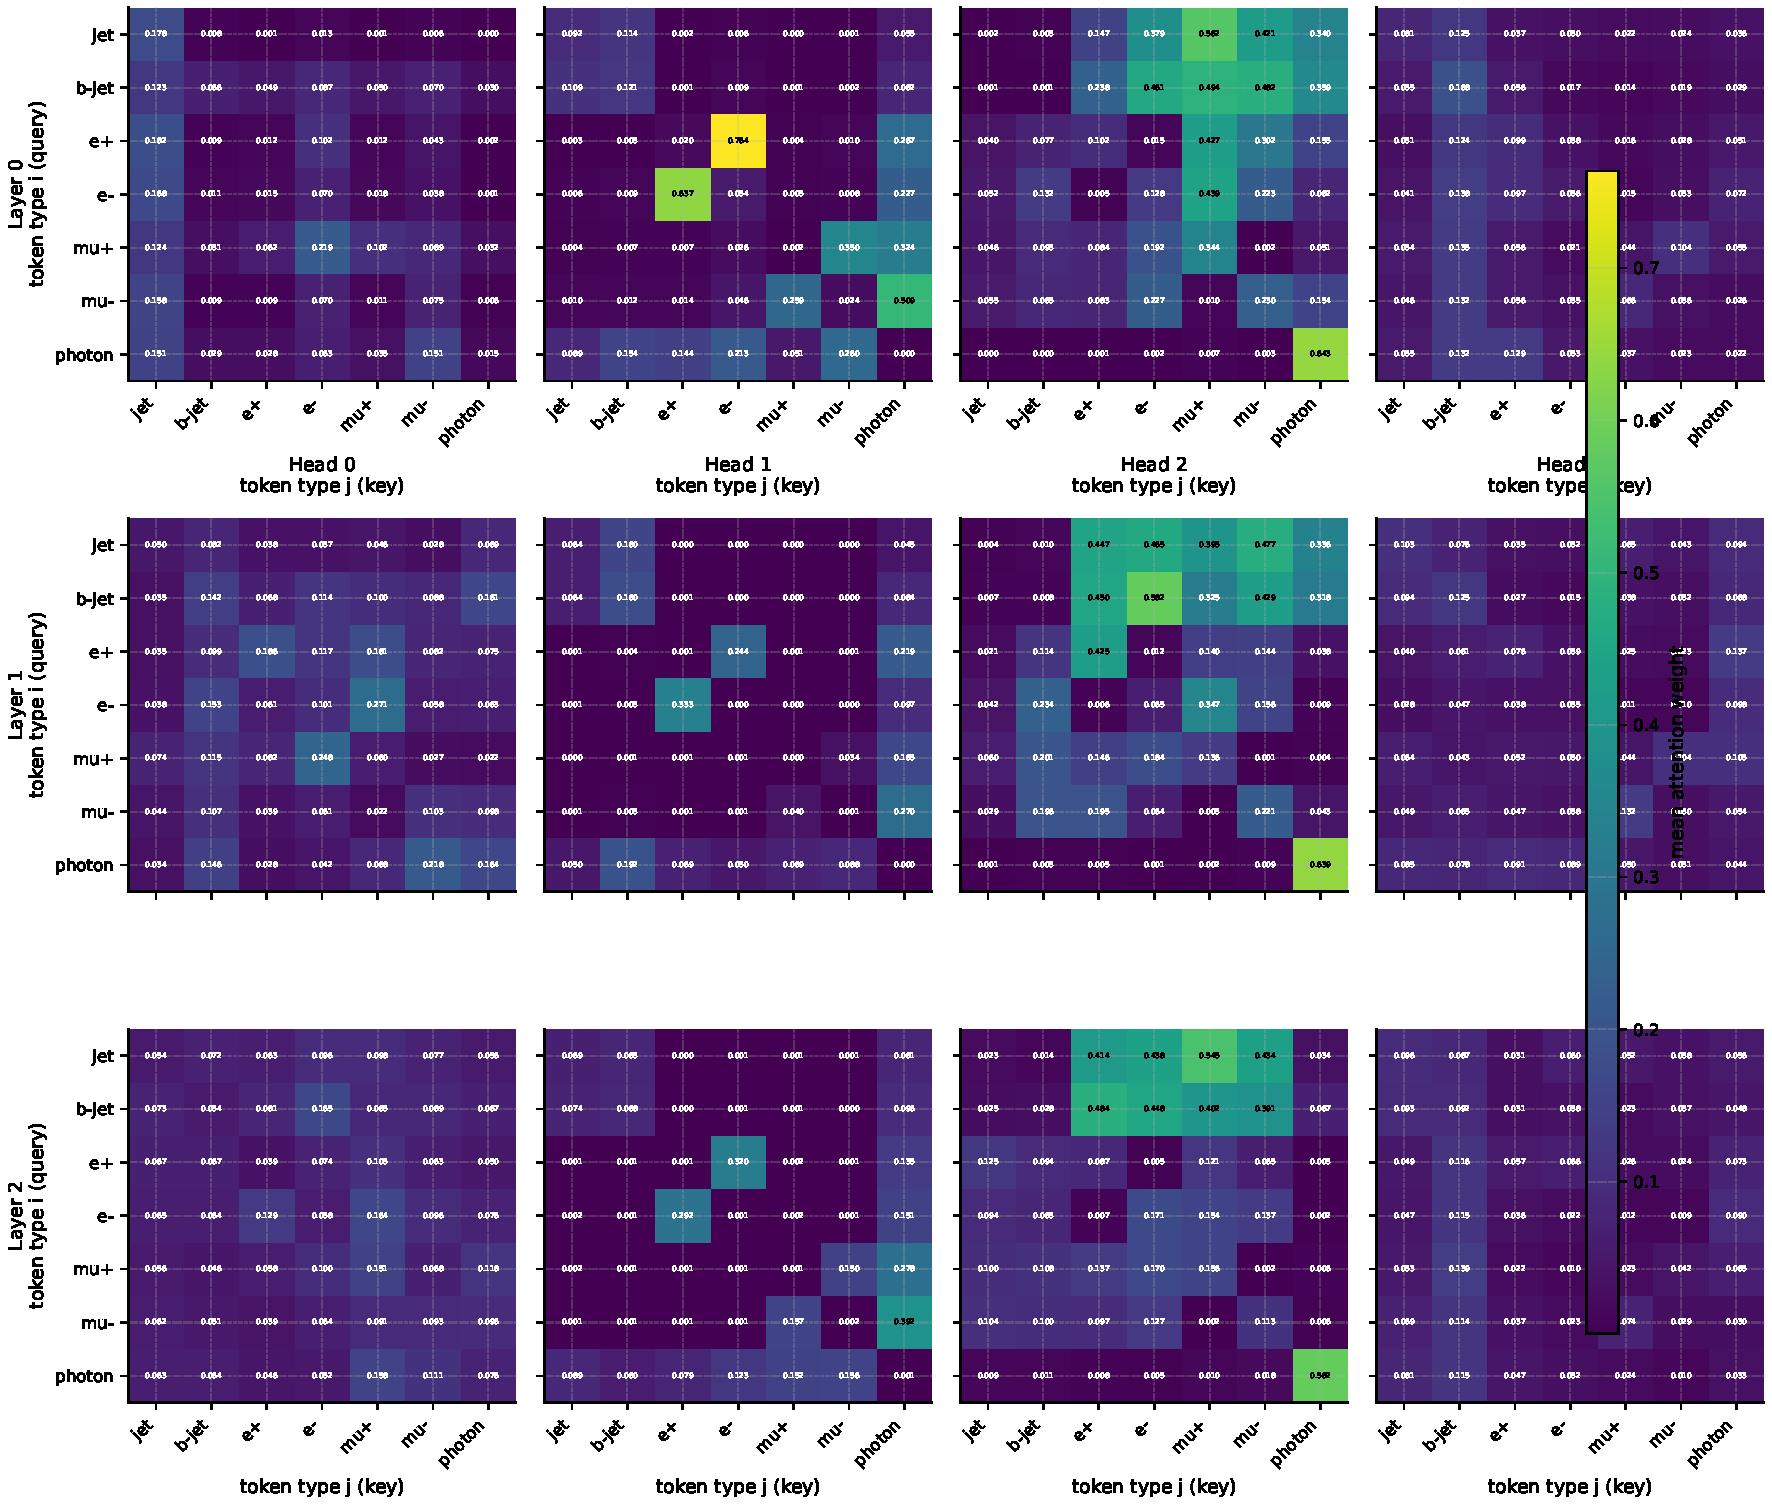
\includegraphics[width=\textwidth]{figures/ch5/figure-attn_typepair_per_head_full}
\caption{Type-pair attention weights for the full-combination model (seed 42),
shown separately for each of the 4 heads $\times$ 3 encoder layers.
Some heads specialise onto physically motivated pairs while others retain
near-uniform attention.}
\label{fig:5a_attn_per_head_full}
\end{figure}

The per-head, per-layer attention grids (available in the supplementary
figures) show that the structured pattern is not uniform across all twelve
head--layer combinations. Some heads retain near-uniform attention while
others specialise strongly onto physically motivated pairs, consistent with
the expectation that multi-head attention allows functional specialisation.


% ──────────────────────────────────────────────
\section{Lorentz feature set and bias network (Exp.\ 5B)}
\label{sec:5b}

\subsection{Experimental design}

The Lorentz-scalar bias sub-network (\wandbaxis{B1-L}) computes a pairwise
attention score from Lorentz-invariant quantities derived from pairs of
four-momenta. Experiment 5B asks three questions about the internal design
of this sub-network: which kinematic features are most informative
(\wandbaxis{B1-L1}), whether replacing the standard pointwise MLP with a
Kolmogorov--Arnold Network (KAN) improves the learned response
(\wandbaxis{B1-L2}), and whether a per-feature sparse gate (\wandbaxis{B1-L5})
can learn to prune uninformative features automatically. Sixty runs span
five feature sets, two MLP types, and two gating settings, at three seeds
each.

\begin{table}[h]
\centering\small
\begin{tabular}{llr}
\toprule
Axis & Values & Levels \\
\midrule
\wandbaxis{B1-L1} — Feature set & \texttt{[deltaR]}                                      & 5 \\
 & \texttt{[m2]}                                         & \\
 & \texttt{[m2, deltaR]}                                 & \\
 & \texttt{[log\_kt, z, deltaR, log\_m2]}               & \\
 & \texttt{[m2, deltaR, log\_m2, log\_kt, z, deltaR\_ptw]} & \\
\wandbaxis{B1-L2} — MLP type    & \texttt{standard}, \texttt{kan}                     & 2 \\
\wandbaxis{B1-L5} — Sparse gating & \texttt{false}, \texttt{true}                     & 2 \\
Seeds (\wandbaxis{R5})           & 42, 123, 314                                          & 3 \\
\midrule
Total & & \textbf{60} \\
\bottomrule
\end{tabular}
\caption{Exp.\ 5B design. B1~=~\texttt{lorentz\_scalar} throughout.
B1-L3 (hidden dim) and B1-L4 (per-head mode) are held at defaults.}
\label{tab:5b_design}
\end{table}

All kinematic features are computed from z-score-normalised four-vectors.
An important consequence of this normalisation is that the pairwise
invariant mass $m^2$ collapses near zero on the normalised scale (validation
median of $m^2$ is $0.000$; 95th percentile is $2.47$). The logarithmic
variant $\log m^2$ collapses further (validation median
$\approx \log(10^{-6}) \approx -13.8$). This means that any claim about
``learning the $W$-boson or top-quark mass peak'' is not supported by these
checkpoints; such an analysis would require either removing input
normalisation or de-normalising the feature axis. By contrast, $\Delta R$,
$\log k_T$, and $z$ remain well-behaved on the normalised scale ($\Delta R$
at the 5th and 95th percentiles: $0.79$ and $4.17$ respectively), and
interpretability arguments based on those features are on firmer ground.

\subsection{AUROC results}

Table~\ref{tab:5b_auroc} reports seed-mean AUROC for all 20 (feature set,
MLP type, gating) cells. The full bar chart is shown as Figure~\ref{fig:5b_auroc_bar}.

\begin{figure}[h]
\centering
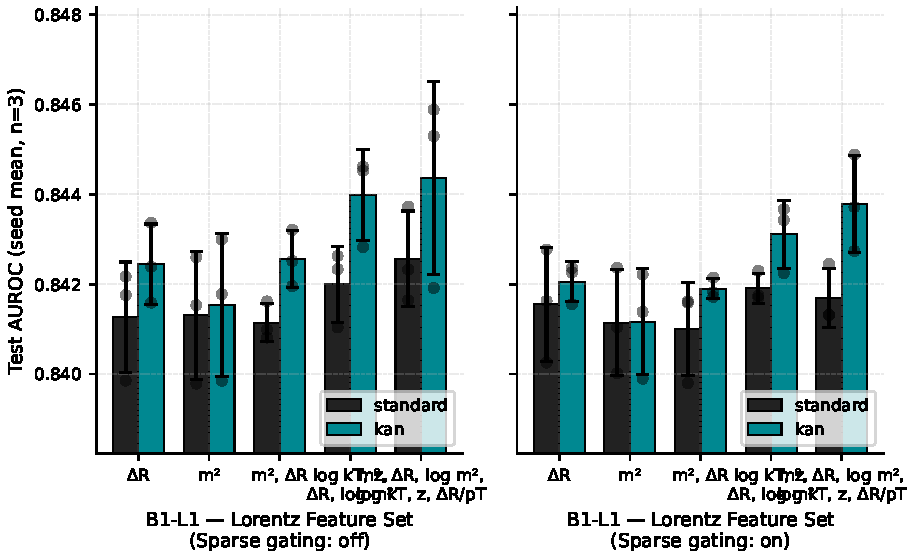
\includegraphics[width=\textwidth]{figures/ch5/figure-auroc_bar_by_lorentz}
\caption{Exp.\ 5B seed-mean test AUROC for all 20 (feature set, MLP type,
gating) cells, with per-seed spread. KAN consistently meets or exceeds the
standard MLP; richer feature sets produce higher AUROC; sparse gating
provides no benefit.}
\label{fig:5b_auroc_bar}
\end{figure}

\begin{table}[h]
\centering\small
\begin{tabular}{llllrr}
\toprule
Feature set & MLP type & Gating & Mean AUROC & Seed std \\
\midrule
$\Delta R$                                & standard & off & 0.84126 & 0.00123 \\
$\Delta R$                                & kan      & off & 0.84245 & 0.00089 \\
$\Delta R$                                & standard & on  & 0.84155 & 0.00126 \\
$\Delta R$                                & kan      & on  & 0.84206 & 0.00044 \\
\addlinespace
$m^2$                                     & standard & off & 0.84131 & 0.00142 \\
$m^2$                                     & kan      & off & 0.84154 & 0.00159 \\
$m^2$                                     & standard & on  & 0.84114 & 0.00118 \\
$m^2$                                     & kan      & on  & 0.84117 & 0.00118 \\
\addlinespace
$m^2$, $\Delta R$                          & standard & off & 0.84114 & 0.00042 \\
$m^2$, $\Delta R$                          & kan      & off & 0.84256 & 0.00063 \\
$m^2$, $\Delta R$                          & standard & on  & 0.84100 & 0.00104 \\
$m^2$, $\Delta R$                          & kan      & on  & 0.84190 & 0.00022 \\
\addlinespace
$\log k_T$, $z$, $\Delta R$, $\log m^2$   & standard & off & 0.84200 & 0.00085 \\
$\log k_T$, $z$, $\Delta R$, $\log m^2$   & kan      & off & 0.84399 & 0.00101 \\
$\log k_T$, $z$, $\Delta R$, $\log m^2$   & standard & on  & 0.84191 & 0.00034 \\
$\log k_T$, $z$, $\Delta R$, $\log m^2$   & kan      & on  & 0.84311 & 0.00076 \\
\addlinespace
$m^2$, $\Delta R$, $\log m^2$, $\log k_T$, $z$, $\Delta R/p_T$  & standard & off & 0.84257 & 0.00106 \\
$m^2$, $\Delta R$, $\log m^2$, $\log k_T$, $z$, $\Delta R/p_T$  & kan      & off & \textbf{0.84436} & 0.00214 \\
$m^2$, $\Delta R$, $\log m^2$, $\log k_T$, $z$, $\Delta R/p_T$  & standard & on  & 0.84170 & 0.00065 \\
$m^2$, $\Delta R$, $\log m^2$, $\log k_T$, $z$, $\Delta R/p_T$  & kan      & on  & 0.84378 & 0.00107 \\
\bottomrule
\end{tabular}
\caption{Exp.\ 5B seed-mean test AUROC ($n = 3$ per cell). The
\texttt{none} baseline from Exp.\ 5A is $0.84125 \pm 0.00068$.
Best cell highlighted. Gating ``on'' = \wandbaxis{B1-L5}~=~\texttt{true}.}
\label{tab:5b_auroc}
\end{table}

Three consistent trends emerge from the table. First, within every
(feature-set, gating) pairing, the \texttt{kan} MLP equals or exceeds the
\texttt{standard} MLP in seed-mean AUROC. The largest gap appears in the
six-feature, gating-off configuration ($+0.0018$ AUROC), which equals
approximately one seed standard deviation. The global best cell (6-feature,
KAN, gate off: $0.84436$) sits roughly $+0.0031$ above the Exp.\ 5A
\texttt{none} baseline ($0.84125$), a margin comparable to several per-cell
seed standard deviations. Second, richer Lorentz feature panels
systematically produce higher AUROC than single-feature panels, particularly
when paired with the KAN. The four- and six-feature sets consistently
outperform the $\Delta R$-only and $m^2$-only single-feature sets; this
trend is visible in both the standard and KAN columns. Third, sparse gating
provides no benefit at this scale and seed budget: gate-on cells tend to
sit slightly below their gate-off counterparts in the same (feature, MLP)
row, by approximately $0.0005$--$0.0009$ AUROC.

\subsection{KAN spline structure and gate values}
\label{sec:5b_interp}

The expressive difference between KAN and standard MLP is visible not only
in AUROC but in the learned attention-bias functions themselves. In the
single-feature ($\Delta R$) configuration with gating off, the seed-mean
bias function spans a range of $0.99$ arbitrary units under the KAN, versus
$0.46$ under the standard MLP: a factor of approximately two. In the
partial-dependence view of the four-feature configuration (other features
held at validation medians), the standard MLP learns almost no log-$k_T$
dependence (range $\approx 0.05$), while the KAN learns a structured curve
with range $\approx 0.65$. This result is consistent with the KAN's
capacity to model sharp univariate edges with a small parameter budget
through its B-spline basis. The KAN therefore extracts more functional
structure from the pairwise kinematic features, which is reflected in the
consistent AUROC advantage.

\begin{figure}[h]
\centering
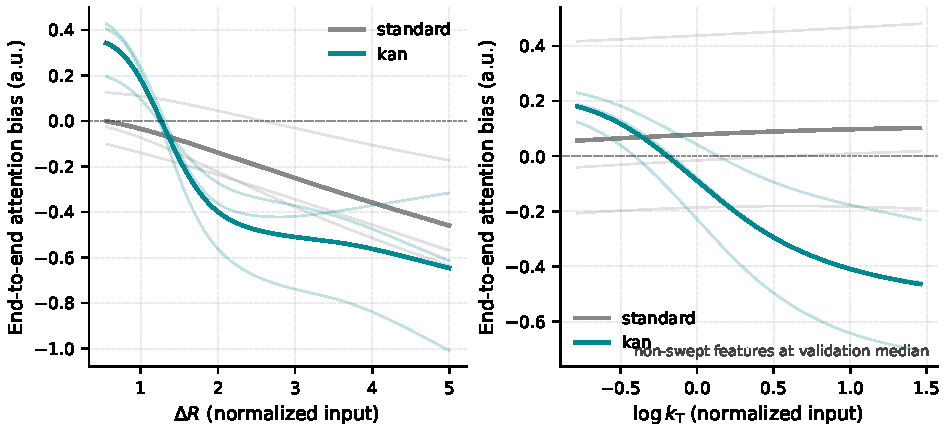
\includegraphics[width=0.7\textwidth]{figures/ch5/figure-1d_bias_kan_vs_standard}
\caption{Learned 1D bias function for the $\Delta R$-only feature set
comparing KAN (blue) and standard MLP (orange), averaged over three seeds.
The KAN spans a range of $\approx 0.99$ attention units versus $\approx 0.46$
for the standard MLP.}
\label{fig:5b_bias_1d}
\end{figure}

The per-module gate, $\tanh(g)$, converged to a positive value in every one
of the 60 Exp.\ 5B runs, confirming that the Lorentz bias is non-trivially
active throughout the cohort. KAN modules average $\tanh(g) \approx 0.28
\pm 0.08$ versus $0.22 \pm 0.10$ for standard modules. The higher gate for
KAN runs echoes the AUROC finding: the network allows more of the KAN's
richer signal through its multiplicative gate.

Despite the gate being consistently open, the sparse feature-gating
mechanism (\wandbaxis{B1-L5}) does not learn meaningful per-feature
selection. The sigmoid gate values $\sigma(\text{feature\_gates})$ remain
within $0.49$--$0.62$ across all 15 sparse-on KAN runs, barely departing
from their initialisation at $\sigma(0) = 0.5$.  The only feature whose
mean gate drifts slightly below $0.5$ is $\log m^2$, which is precisely
the feature whose input distribution collapses near $-13.8$ under z-score
normalisation. Even this drift is modest ($\approx 0.494 \pm 0.022$),
and no feature is pruned in any run. The effect on AUROC is therefore a
slight attenuation of every feature's amplitude simultaneously, with no
compensating benefit from pruning, which explains the small but systematic
gap between gate-on and gate-off cells.

\begin{figure}[h]
\centering
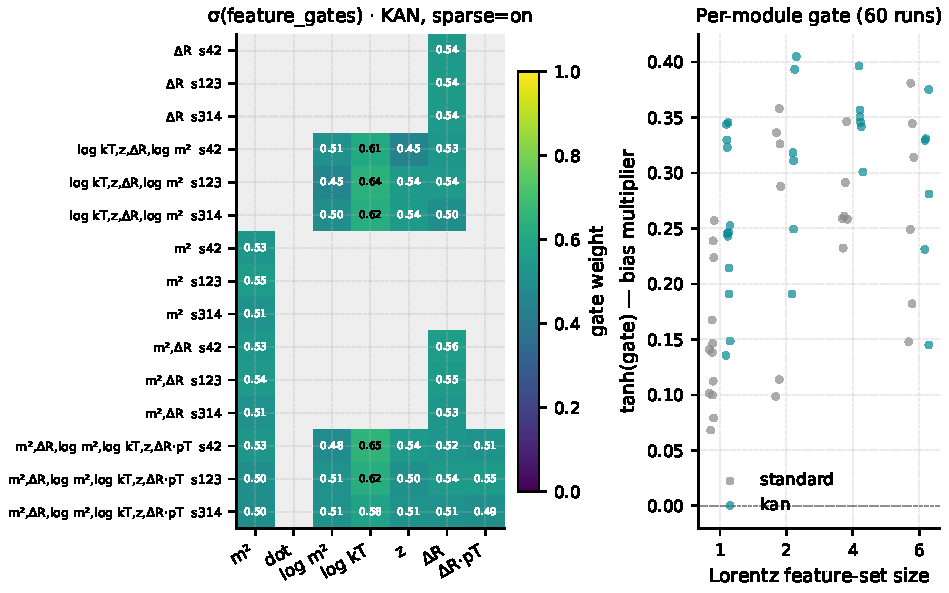
\includegraphics[width=\textwidth]{figures/ch5/figure-feature_gates_and_module_gate}
\caption{Left: per-feature sparse gate values $\sigma(\text{gate})$ for all
Exp.\ 5B sparse-on KAN runs; all gates remain within $0.49$--$0.62$,
indicating no meaningful feature pruning. Right: module-level scalar gate
$\tanh(g)$ for KAN (blue) and standard (orange) MLP runs across the full
cohort.}
\label{fig:5b_gates}
\end{figure}

One caveat for the spline-shape analysis is that the KAN B-spline grid is
fixed at its initialisation throughout training: \texttt{update\_grid} is
not called during the forward pass, which was confirmed by state-dict
inspection of the \texttt{mlp.0.grid} key in the saved checkpoints. The
spline expressivity is therefore bounded by the initial grid resolution
and not by adaptive grid relocation. More adaptive grid training could in
principle widen the gap further.


% ──────────────────────────────────────────────
\section{Type-pair initialisation and freeze (Exp.\ 5C)}
\label{sec:5c}

\subsection{Experimental design}

The type-pair kinematic bias (\wandbaxis{B1-T}) maintains a learnable
$N_\mathrm{type}\times N_\mathrm{type}$ table of attention score offsets,
one per ordered particle-type pair. Experiment 5C varies two design choices:
the initialisation strategy (\wandbaxis{B1-T1}) and whether the table is
frozen after initialisation (\wandbaxis{B1-T2}). Three initialisation
modes are tested: \texttt{none} (zero start, free to train), \texttt{binary}
(a $\{0, -5\}$ mask encoding which SM vertices are allowed or forbidden),
and \texttt{fixed\_coupling} (the physics-motivated initialisation, with
magnitudes proportional to SM coupling constants). A frozen table
(\texttt{freeze\_table~=~true}) acts as a fixed physics prior; a free
table is adjusted by gradient descent from its initialised state. Fifteen
runs cover five cells (the \texttt{none}--frozen combination is excluded,
as there is no table to freeze) at three seeds each.

\begin{table}[h]
\centering\small
\begin{tabular}{llr}
\toprule
Axis & Values & Levels \\
\midrule
\wandbaxis{B1-T1} — Init & \texttt{none}, \texttt{binary}, \texttt{fixed\_coupling} & 3 \\
\wandbaxis{B1-T2} — Freeze & \texttt{false}, \texttt{true} (only when init $\neq$ \texttt{none}) & — \\
Seeds (\wandbaxis{R5})     & 42, 123, 314 & 3 \\
\midrule
Total & & \textbf{15} \\
\bottomrule
\end{tabular}
\caption{Exp.\ 5C design. B1~=~\texttt{typepair\_kinematic} throughout.
B1-T3 (kinematic gate), B1-T4 (kinematic feature), and B1-T5 (mask value)
are held at defaults.}
\label{tab:5c_design}
\end{table}

\subsection{Performance results}

Table~\ref{tab:5c_auroc} reports seed-mean AUROC for the five cells.
The local \texttt{none}-init baseline here (0.84205) is slightly above the
Exp.\ 5A \texttt{none} cell (0.84125), a difference attributable to the
different sweep configuration and cohort, not to a change in the architecture.

\begin{table}[h]
\centering\small
\begin{tabular}{lllrrl}
\toprule
Init & Freeze & Mean AUROC & Seed std & $\Delta$ vs \texttt{none} \\
\midrule
\texttt{none}           & free   & 0.84205 & 0.00081 & --- \\
\texttt{binary}         & free   & 0.84075 & 0.00046 & $-0.00130$ \\
\texttt{binary}         & frozen & 0.84131 & 0.00065 & $-0.00074$ \\
\texttt{fixed\_coupling}& free   & 0.84175 & 0.00102 & $-0.00030$ \\
\texttt{fixed\_coupling}& frozen & 0.84138 & 0.00046 & $-0.00067$ \\
\bottomrule
\end{tabular}
\caption{Exp.\ 5C seed-mean test AUROC ($n = 3$ per cell). All four
physics-initialised cells sit below the \texttt{none} baseline within one
to two seed standard deviations.}
\label{tab:5c_auroc}
\end{table}

All four physics-initialised cells sit below the \texttt{none} baseline in
seed mean, by margins of $0.0003$--$0.0013$ AUROC. These deltas are within
one to two per-cell seed standard deviations and should not be interpreted
as a meaningful performance deficit. The \texttt{fixed\_coupling}
initialisation consistently outperforms \texttt{binary} by approximately
$0.0006$--$0.0010$ AUROC regardless of freeze state, but again at the noise
floor. Freezing the table has small, non-monotonic effects: it slightly
improves \texttt{binary} ($+0.00056$) and slightly reduces
\texttt{fixed\_coupling} ($-0.00037$), both within seed variance.

The AUROC results therefore suggest neither a benefit from SM-seeded
initialisation nor a cost from freezing the physics prior, at this seed
budget and model scale.

\subsection{Learned table structure}

The more informative view comes from inspecting the converged type-pair
tables directly. The state-dict key
\texttt{bias\_composer.bias\_modules.\allowbreak{}typepair\_kinematic.\allowbreak{}table\_raw}
has shape $[8,8]$; the symmetric form is reconstructed as
$\frac{1}{2}(T + T^\top)$ and the padding row and column are removed,
leaving a $7\times 7$ active matrix. Table~\ref{tab:5c_table_stats}
summarises key scalar statistics.

\begin{table}[h]
\centering\small
\begin{tabular}{llrlrl}
\toprule
Init & Freeze & Gate ($\tanh g$, mean $\pm$ std) & Frobenius norm & Drift from init \\
\midrule
\texttt{none}            & free   & $0.234 \pm 0.015$ & 0.434  & 0.944 (= norm) \\
\texttt{binary}          & free   & $0.097 \pm 0.012$ & 27.044 & 0.868 \\
\texttt{binary}          & frozen & $0.094 \pm 0.013$ & 27.295 & 0.000 (frozen) \\
\texttt{fixed\_coupling} & free   & $0.104 \pm 0.015$ & 26.848 & 0.930 \\
\texttt{fixed\_coupling} & frozen & $0.101 \pm 0.015$ & 27.094 & $\approx 0$ \\
\bottomrule
\end{tabular}
\caption{Exp.\ 5C per-group learned-table statistics. Gate = $\tanh(g)$
averaged over 3 seeds. Frobenius norm computed on the $7\times 7$ active
sub-matrix. Drift from init = Frobenius distance between the converged
seed-mean table and the reference initialisation.}
\label{tab:5c_table_stats}
\end{table}

The \texttt{none}-init table starts from zero and converges to a
small-magnitude matrix (Frobenius $0.43$), with values scattered in
$[-0.16, +0.12]$ showing no discernible SM-interaction pattern at $n=3$
seeds. Its gate is notably higher ($0.234$) than any physics-initialised
group ($0.094$--$0.104$), consistent with the network opening the gate
further when the table provides a weak prior and all type pairs look equally
neutral at initialisation.

The \texttt{fixed\_coupling}-free table preserves the SM structure through
training. QCD quark--quark pairs (jet--jet: $+1.22$, jet--b-jet: $+1.17$,
b-jet--b-jet: $+1.23$) retain large positive values; EW lepton pairs
($e^+e^-$: $+0.54$, $\mu^+\mu^-$: $+0.89$) retain intermediate positive
values; and all non-interacting pairs remain near the mask value of $-5.0$.
The Frobenius drift from initialisation is $0.930$, indicating that
training adjusts the coupling-constant magnitudes by roughly $\pm 0.1$--$0.3$
rather than restructuring the topology. This is a notable result: the
network broadly respects the SM interaction hierarchy encoded at
initialisation, even when the gradient is free to reorganise the table
entirely.

\begin{figure}[h]
\centering
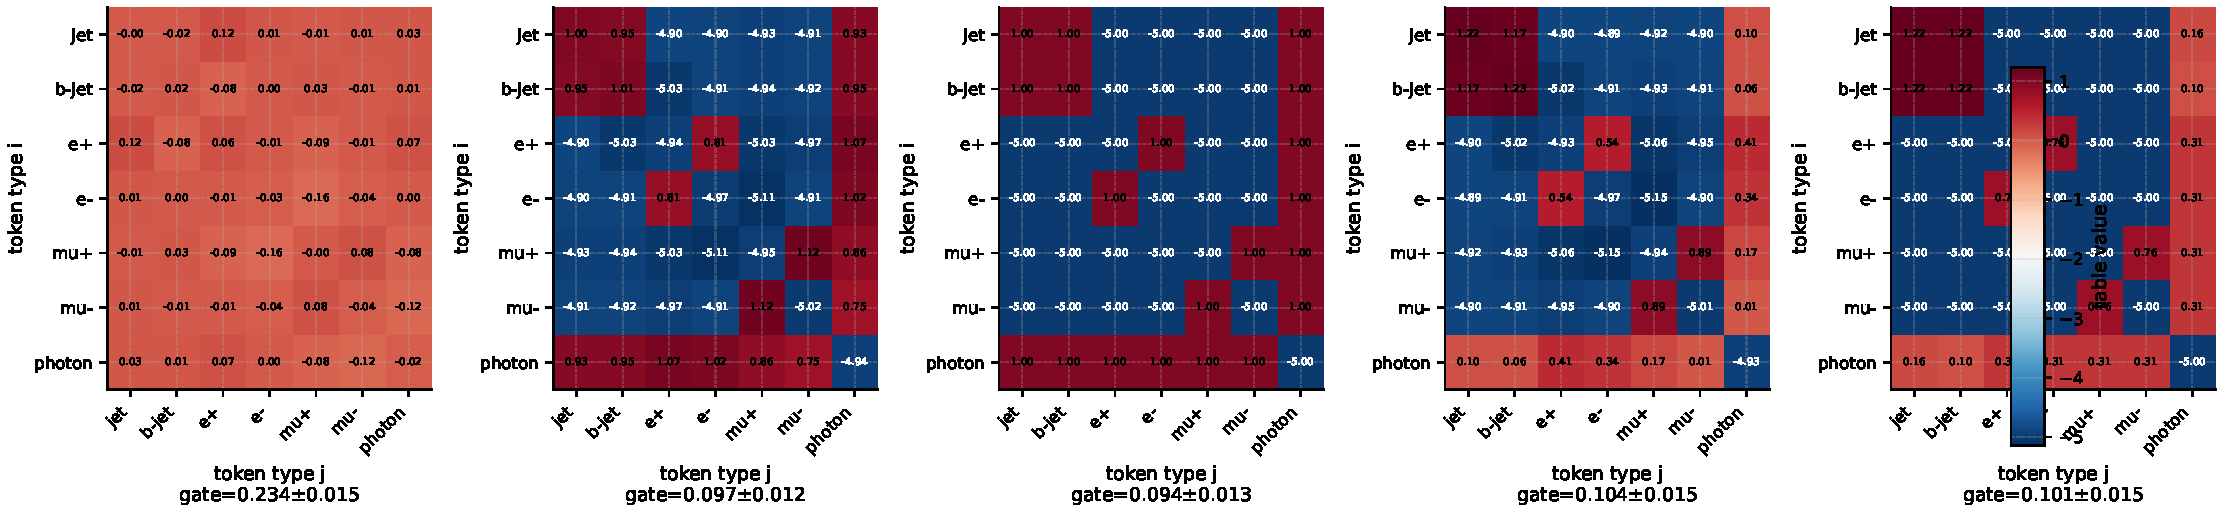
\includegraphics[width=\textwidth]{figures/ch5/figure-typepair_learned_tables}
\caption{Converged type-pair tables ($7\times 7$ active sub-matrix) for all
five Exp.\ 5C groups, averaged over three seeds. The
\texttt{fixed\_coupling}-free table preserves the SM coupling hierarchy;
the \texttt{none}-init table remains near-uniform.}
\label{fig:5c_tables}
\end{figure}

\begin{figure}[h]
\centering
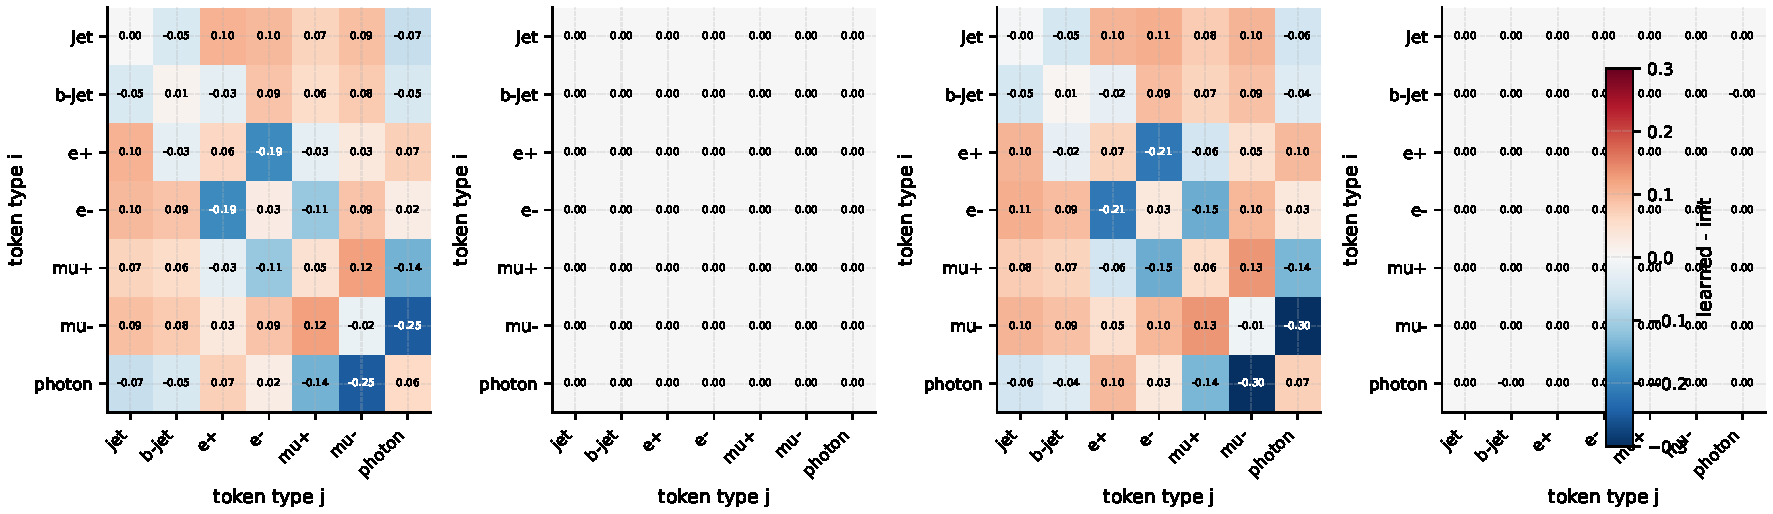
\includegraphics[width=\textwidth]{figures/ch5/figure-typepair_diff_from_init}
\caption{Per-cell table drift from initialisation for the free-table groups.
\texttt{fixed\_coupling}-free (top) shows small, structured adjustments
($\pm 0.1$--$0.3$) with the SM topology intact;
\texttt{binary}-free (bottom) shows larger drift at active entries.}
\label{fig:5c_diff}
\end{figure}

The \texttt{binary}-free group shows an analogous pattern (same mask
positions preserved) but with higher drift (0.868 vs 0.930), reflecting the
fact that the binary initialisation provides structural topology but no
coupling-constant scale, leaving active entries more exposed to gradient
learning. The frozen groups confirm the mechanism functions correctly
(freeze drift $\approx 6.6 \times 10^{-8}$ for \texttt{fixed\_coupling}-frozen).

Taken together, the results suggest that the SM \texttt{fixed\_coupling}
initialisation provides a structural prior that training broadly preserves,
but that its effective attention contribution, modulated by the scalar gate
($\tanh(g) \approx 0.10$), is too small to produce a measurable AUROC
improvement at this configuration. The \texttt{none}-init group, starting
from a flat table, fails to recover a physics-consistent structure at three
seeds --- the table remains near-uniform, indicating that the inductive bias
from the initialisation is important for guiding the table to a structured
solution.


% ──────────────────────────────────────────────
\section{SM interaction mode (Exp.\ 5D)}
\label{sec:5d}

Experiment 5D tests whether increasing physical fidelity in the SM
interaction prior produces measurable gains. The \texttt{sm\_interaction}
bias family encodes SM topology as a fixed or modulated additive bias on
attention logits; axis \wandbaxis{B1-S1} selects among three modes:
\texttt{binary} (a $\{0, -5\}$ allowed/forbidden mask), \texttt{fixed\_coupling}
(coupling constants at a fixed energy scale), and
\texttt{running\_coupling} ($\alpha_s(Q^2)$ evaluated at the pairwise
momentum transfer). Nine runs cover all three modes at three seeds each.

\begin{table}[h]
\centering\small
\begin{tabular}{llr}
\toprule
Axis & Values & Levels \\
\midrule
\wandbaxis{B1-S1} — SM mode & \texttt{binary}, \texttt{fixed\_coupling}, \texttt{running\_coupling} & 3 \\
Seeds (\wandbaxis{R5})       & 42, 123, 314 & 3 \\
\midrule
Total & & \textbf{9} \\
\bottomrule
\end{tabular}
\caption{Exp.\ 5D design. B1~=~\texttt{sm\_interaction} throughout.
B1-S2 (mask value) held at default.}
\label{tab:5d_design}
\end{table}

Table~\ref{tab:5d_auroc} reports seed-mean AUROC. The reference \texttt{none}
baseline from Exp.\ 5A ($0.84125 \pm 0.00068$) is used for comparison, as
Exp.\ 5D does not include an explicit \texttt{none} cell; both cohorts
share the same encoder hyperparameters and seed list, so the cross-cohort
comparison is reasonable.

\begin{table}[h]
\centering\small
\begin{tabular}{lrrl}
\toprule
B1-S1 mode & Mean AUROC & Seed std & $\Delta$ vs 5A \texttt{none} \\
\midrule
\texttt{binary}           & 0.84140 & 0.00050 & $+0.00015$ \\
\texttt{fixed\_coupling}  & 0.84146 & 0.00091 & $+0.00021$ \\
\texttt{running\_coupling}& 0.84108 & 0.00081 & $-0.00018$ \\
\bottomrule
\end{tabular}
\caption{Exp.\ 5D seed-mean test AUROC ($n = 3$ per cell). All three modes
are within $\pm 0.0002$ AUROC of the Exp.\ 5A \texttt{none} baseline.}
\label{tab:5d_auroc}
\end{table}

All three SM-interaction modes sit within $\pm 0.0002$ AUROC of the
\texttt{none} baseline, and the three modes span only $\approx 0.0004$
AUROC among themselves. Both magnitudes are at or below the per-cell seed
standard deviation, making no mode distinguishable from another within this
seed budget. The nominal ranking (\texttt{fixed\_coupling} $>$
\texttt{binary} $>$ \texttt{running\_coupling}) is consistent with the
\texttt{running\_coupling} mode being the most parameter-rich and therefore
most exposed to optimisation noise at fixed hyperparameters, but this
interpretation should not be treated as a directional finding at $n=3$ seeds.

\begin{figure}[h]
\centering
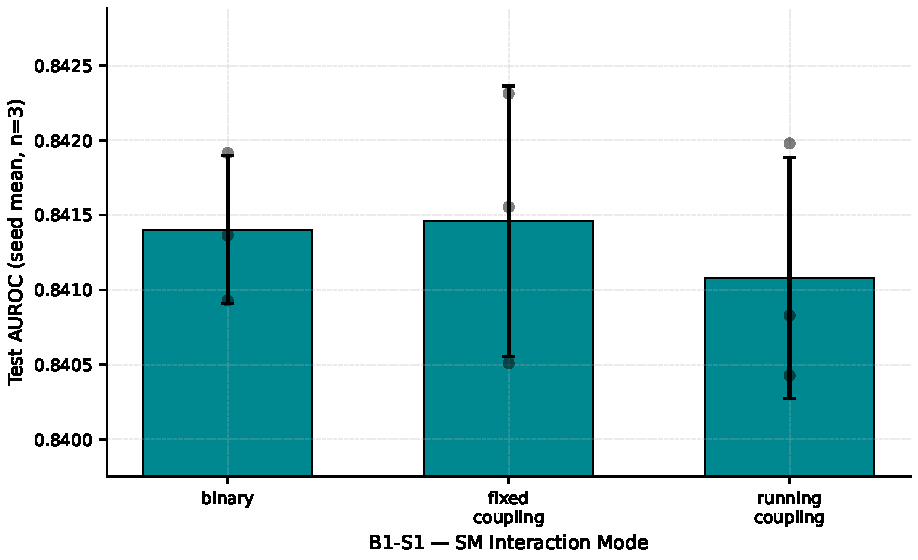
\includegraphics[width=0.7\textwidth]{figures/ch5/figure-auroc_bar_by_sm_mode}
\caption{Exp.\ 5D seed-mean test AUROC for the three \wandbaxis{B1-S1}
modes, with per-seed spread. Dashed line marks the Exp.\ 5A
\texttt{none} baseline. All three modes are within $\pm 0.0002$ AUROC of
the baseline.}
\label{fig:5d_auroc_bar}
\end{figure}

The SM interaction prior as implemented in Exp.\ 5D is therefore a null
result on the AUROC axis at this model scale. Whether the prior is active
in the attention pattern is a question for a future attention-map follow-up
analogous to the Exp.\ 5A analysis (currently staged but not yet run).
For the purpose of the downstream best-model selection in Ch.\,8, the
\texttt{fixed\_coupling} mode is carried forward as the default SM setting
on the grounds of physical motivation, accepting that the performance
difference is negligible.


% ──────────────────────────────────────────────
\section{Chapter synthesis}
\label{sec:5_synthesis}

This chapter set out to ask whether physics-informed attention biases
improve 4-tops-versus-background classification, and what those biases
reveal about the model's internal organisation of particle relationships.
The AUROC results across all four sub-experiments are consistent and
unambiguous: no single bias family, and no configuration within any
family, produces a performance gain that is clearly separable from seed
variance at $n=3$ seeds per cell. The total AUROC range across all 102
runs is approximately $0.838$--$0.846$, with per-cell seed standard
deviations of order $0.001$. The full-combination configuration in Exp.\ 5A
is the only cell that sits visibly below the \texttt{none} baseline
($\approx -0.002$ AUROC), suggestive of optimisation interference from
multiple simultaneous bias signals.

The interpretability results tell a richer story. When all four bias
families are active, the model sharpens type-pair attention onto
physically motivated particle relationships: the attention range widens by
a factor of $2.6$ (from $0.054$ in the \texttt{none} baseline to $0.139$
in the full-combination model), and the most elevated pairs are lepton--photon
($\mu^- \to \gamma$: $0.178$), photon self-attention ($0.164$), b-jet-to-muon
pairs consistent with semi-leptonic $b$-decay ($0.142$, $0.133$), and
opposite-sign lepton pairs consistent with $Z/W$ decay ($e^- \to e^+$:
$0.139$). Same-charge mixed-lepton pairs, which lack a common SM vertex,
are strongly suppressed. These patterns demonstrate that physics-informed
biases restructure the model's attention rather than merely adding capacity.

Within the Lorentz-scalar family, KAN sub-networks consistently learn
richer bias functions than standard MLPs across the same feature sets,
with the largest gap at the six-feature configuration ($+0.0018$ AUROC,
bias-function range $2\times$ wider). Sparse feature gating, however,
converges to the all-open state ($\sigma \approx 0.5$) in every run,
providing no automatic feature selection at this training budget.

The type-pair table analysis shows that the SM \texttt{fixed\_coupling}
initialisation provides a structural prior that training broadly respects:
QCD quark--quark and EW lepton-pair entries retain their physics-consistent
magnitudes through gradient descent, with Frobenius drift $0.930$ from the
initialisation. By contrast, a zero-start (\texttt{none}-init) table fails
to recover a physics-consistent structure at $n=3$ seeds, suggesting that
the inductive bias from a physics-motivated initialisation is beneficial
for interpretability even when it does not shift accuracy.

The practical takeaway for the remainder of the thesis is that
physics-informed attention biases do not change the operating point of the
classifier at the model scale studied in this chapter. Their value is
interpretive: they make the model's attention patterns legible in HEP
terms. For downstream experiments in Ch.\,6 and Ch.\,8, the chapter
baseline carries forward the \texttt{lorentz\_scalar} bias in the
six-feature, standard-MLP, gating-off configuration as the default B1
setting, on the grounds that it provides the most consistent, modest AUROC
benefit without the optimisation risk of the full-combination stack.

\begin{table}[h]
\centering\small
\begin{tabular}{llr}
\toprule
Experiment & Primary axes & Runs \\
\midrule
5A — Family comparison    & \wandbaxis{B1}                            & 18 \\
5B — Lorentz ablation     & \wandbaxis{B1-L1}, \wandbaxis{B1-L2}, \wandbaxis{B1-L5} & 60 \\
5C — Type-pair table      & \wandbaxis{B1-T1}, \wandbaxis{B1-T2}      & 15 \\
5D — SM interaction mode  & \wandbaxis{B1-S1}                         &  9 \\
\midrule
\textbf{Total} & & \textbf{102} \\
\bottomrule
\end{tabular}
\caption{Chapter 5 run summary.}
\label{tab:ch5_summary}
\end{table}

\chapter{Attention Mechanisms}

The attention mechanism is the only component that operates over all
token pairs simultaneously. Chapters 4 and 5 asked how to enrich the
information arriving at the attention layer; this chapter asks whether
the attention computation itself should be modified. The central
question is whether differential attention,which computes the
difference of two softmax maps to suppress diffuse, low-information
attention patterns, transfers from its original NLP setting to
particle classification.

The physics motivation is direct: in a multi-top event, only a small
subset of the 10--20 reconstructed objects are decay products of the
four top quarks. Standard softmax attention distributes probability
mass across all token pairs including unrelated soft objects.
Differential attention is designed for exactly this setting, and
provides a clear testable hypothesis.

Two experiments are run. Exp.\ 6A establishes the headline comparison
across attention type, internal normalisation, and the presence of a
Lorentz-scalar bias. Exp.\ 6B is a targeted follow-up on how physics
biases interact with the two differential attention branches.

% ──────────────────────────────────────────────
\section{Attention type and internal normalisation (Exp.\ 6A)}
\textit{Lens: performance and efficiency.}

Sweeps A3 (standard vs.\ differential), A4 (attention-internal
normalisation), and whether a Lorentz-scalar bias is active. The bias
inclusion tests whether physics structure in the attention logits and
noise suppression from differential attention are complementary or
redundant. Wall-clock time per epoch is recorded alongside AUROC, since
differential attention runs two softmax passes per head.

\begin{table}[h]
\centering\small
\begin{tabular}{llr}
\toprule
Axis & Values & Config \\
\midrule
A3 — Attention type & \texttt{standard}, \texttt{differential} & 2 \\
A4 — Internal norm  & \texttt{none}, \texttt{layernorm}, \texttt{rmsnorm} & 3 \\
B1 — Lorentz bias   & \texttt{none}, \texttt{lorentz\_scalar} & 2 \\
Seeds & & 3 \\
\midrule
Total & & \textbf{36} \\
\bottomrule
\end{tabular}
\caption{Exp.\ 6A. All other axes at chapter baseline.
\texttt{lorentz\_scalar} uses the best feature set from Ch.\,5.}
\end{table}

Outputs: seed-averaged AUROC bar chart for all 12 configurations, with
wall-clock time as a secondary axis. Attention maps extracted at
inference time for standard and differential (both with A4=none,
B1=none), averaged over a fixed held-out batch and labelled by particle
type. If differential attention is working as intended, maps should show
higher concentration on physically proximate pairs.

% ──────────────────────────────────────────────
\section{Differential bias mode (Exp.\ 6B)}
\textit{Lens: performance.}

Restricted to A3=\texttt{differential}. Tests how the additive
Lorentz-scalar bias from Ch.\,5 should interact with the two attention
branches: added to neither, shared across both, or split with separate
parameters per branch.

\begin{table}[h]
\centering\small
\begin{tabular}{llr}
\toprule
Axis & Values & Config \\
\midrule
A3-a — Diff bias mode & \texttt{none}, \texttt{shared}, \texttt{split} & 3 \\
Seeds & & 3 \\
\midrule
Total & & \textbf{9} \\
\bottomrule
\end{tabular}
\caption{Exp.\ 6B. A3=\texttt{differential} and
B1=\texttt{lorentz\_scalar} fixed throughout.}
\end{table}

Output: compact three-row AUROC table. If \texttt{shared} and
\texttt{split} perform equivalently, the second branch does not require
independent bias information and the simpler shared parameterisation
is sufficient.

\subsection*{Chapter summary}

\begin{table}[h]
\centering\small
\begin{tabular}{llr}
\toprule
Experiment & Primary axes & Runs \\
\midrule
6A — Attention type and norm & A3, A4, B1 & 36 \\
6B — Differential bias mode  & A3-a        &  9 \\
\midrule
\textbf{Total} & & \textbf{45} \\
\bottomrule
\end{tabular}
\end{table}


\chapter{Model Scaling and Efficiency}

Every architectural finding in Chapters~4--6 was established at a single, fixed model size. This chapter examines how classifier performance and inference cost vary across a factor of roughly 140 in parameter count, from approximately 26k to 3.6M parameters. Two questions motivate this study. First, where does AUROC saturate as a function of model capacity, and does the saturation point shift with task difficulty? Second, which configuration is Pareto-optimal when performance is weighed against inference cost? The answers retrospectively validate the fixed size used throughout Chapters~4--6 and identify a practical operating point for the evaluation in Chapter~8.

The chapter is structured as follows. Section~\ref{sec:ch7_design} describes the experimental design, which is a full factorial sweep of five model-size presets across three classification tasks (Exp.~7A). Section~\ref{sec:ch7_scaling} reports performance as a function of model size and training cost. Section~\ref{sec:ch7_pareto} presents the Pareto analysis across four efficiency dimensions (Exp.~7B). Section~\ref{sec:ch7_summary} summarises the findings.

% ──────────────────────────────────────────────
\section{Experimental Design}
\label{sec:ch7_design}

All 45 runs in this chapter share a common fixed baseline configuration: tokenizer family \texttt{identity} (axis T1), the feature set D01 selected in Chapter~4, sinusoidal positional encoding (E1 = \texttt{sinusoidal}), standard attention (A3 = \texttt{standard}), LayerNorm with pre-norm policy (A1, A2), and no physics-informed attention biases (B1 = \texttt{none}). Model capacity is the sole variable, swept via the convenience label axis \wandbaxis{H10}, which bundles model dimension (\wandbaxis{H01}), encoder depth (\wandbaxis{H02}), attention heads (H03), and FFN hidden dimension (H04) into five named presets. Three random seeds per cell (axis R05) give 45 runs in total.

\begin{table}[h]
\centering\small
\caption{Exp.~7A design. All other axes held at their thesis baseline values.}
\label{tab:ch7_design}
\begin{tabular}{lll}
\toprule
Axis & Values & Cells \\
\midrule
Model size (\wandbaxis{H10}) & \texttt{d32\_L3}, \texttt{d32\_L5}, \texttt{d64\_L6},
                              \texttt{d128\_L8}, \texttt{d192\_L12} & 5 \\
Task (G03)       & 4t\,vs.\,background, 4t\,vs.\,ttH, multiclass & 3 \\
Seed (R05)       & 3 per cell & 3 \\
\midrule
Total & & \textbf{45} \\
\bottomrule
\end{tabular}
\end{table}

Table~\ref{tab:ch7_sizes} lists the concrete dimension and depth values for each preset, together with the approximate parameter count and analytic FLOPs per event. Analytic FLOPs count multiply-add operations derived from the model architecture; they do not include Python overhead or data-movement costs, but provide a clean, hardware-independent comparison basis.

\begin{table}[h]
\centering\small
\caption{Model-size presets used in Exp.~7A. Approximate parameter counts are derived from H01 and H02; FLOPs per event are analytic multiply-add counts averaged over all 9 runs sharing that preset.}
\label{tab:ch7_sizes}
\begin{tabular}{lrrrl}
\toprule
Size label (H10) & dim (H01) & depth (H02) & Approx.\ params & FLOPs/event (analytic) \\
\midrule
\texttt{d32\_L3}   & 32  & 3  & $\sim$26k   & 1.29M \\
\texttt{d32\_L5}   & 32  & 5  & $\sim$43k   & 2.15M \\
\texttt{d64\_L6}   & 64  & 6  & $\sim$202k  & 10.3M \\
\texttt{d128\_L8}  & 128 & 8  & $\sim$1.06M & 55.1M \\
\texttt{d192\_L12} & 192 & 12 & $\sim$3.57M & 185.8M \\
\bottomrule
\end{tabular}
\end{table}

The jump in FLOPs from \texttt{d64\_L6} to \texttt{d128\_L8} is approximately $\times 5.3$, and from \texttt{d64\_L6} to \texttt{d192\_L12} approximately $\times 18$. This non-linear growth is driven by the quadratic attention cost and the multiplicative effect of simultaneously increasing both depth and width.

% ──────────────────────────────────────────────
\section{Scaling Curves (Exp.\ 7A)}
\label{sec:ch7_scaling}

\subsection{AUROC versus Model Size}

Figure~\ref{fig:ch7_auroc} shows AUROC as a function of model size, separately for each task and aggregated over all three tasks. The aggregated mean and standard deviation over all nine runs (three tasks $\times$ three seeds) per size are reported in Table~\ref{tab:ch7_auroc}.

\begin{figure}[h]
  \centering
  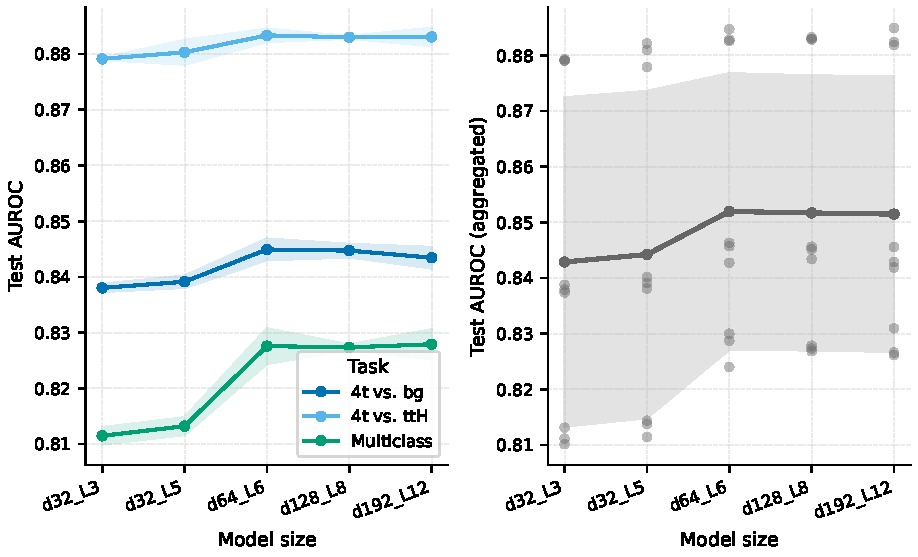
\includegraphics[width=\linewidth]{figures/ch7/ch7_auroc_vs_model_size.pdf}
  \caption{AUROC versus model-size preset for all three tasks (left) and aggregated over tasks with seed scatter (right); higher AUROC is better, and the plateau at \texttt{d64\_L6} is visible in both panels.}
  \label{fig:ch7_auroc}
\end{figure}

\begin{table}[h]
\centering\small
\caption{Aggregated AUROC by model-size preset (mean $\pm$ std over all 9 runs, 3 tasks $\times$ 3 seeds). The large standard deviation reflects cross-task variance, not seed noise; within a single task, seed-to-seed variation is substantially smaller.}
\label{tab:ch7_auroc}
\begin{tabular}{lrr}
\toprule
Size label (H10) & Mean AUROC & Std \\
\midrule
\texttt{d32\_L3}   & 0.843 & 0.030 \\
\texttt{d32\_L5}   & 0.844 & 0.029 \\
\texttt{d64\_L6}   & 0.852 & 0.025 \\
\texttt{d128\_L8}  & 0.852 & 0.025 \\
\texttt{d192\_L12} & 0.852 & 0.025 \\
\bottomrule
\end{tabular}
\end{table}

AUROC rises by approximately 0.8--1.3 percentage points between the two smallest presets and \texttt{d64\_L6}, but the three larger configurations (\texttt{d64\_L6}, \texttt{d128\_L8}, \texttt{d192\_L12}) are statistically indistinguishable at $0.852 \pm 0.025$. The plateau is consistent across all three tasks in the per-task panel. Although the multiclass task yields systematically lower absolute AUROC than the binary tasks (owing to the harder five-class discriminant), the saturation point does not shift: all three tasks plateau at \texttt{d64\_L6}.

The saturation at this relatively small scale is consistent with the low-multiplicity nature of the classification problem. Events in the 4t and ttH samples contain at most a few tens of reconstructed objects, so the information content available per event is modest, and a model with $\sim$202k parameters appears sufficient to extract it with the baseline architecture.

\paragraph{Signal efficiency at fixed background rejection.}

For the two binary tasks, signal efficiency $\varepsilon_S$ at a fixed background rejection of $1/B = 50$ provides a physics-operational complement to AUROC. This metric is undefined for the multiclass task and is not reported there. Table~\ref{tab:ch7_eps} summarises the results.

\begin{table}[h]
\centering\small
\caption{Signal efficiency $\varepsilon_S$ at background rejection $1/B = 50$, for the two binary tasks (mean $\pm$ std over 3 seeds). The plateau pattern mirrors the AUROC result.}
\label{tab:ch7_eps}
\begin{tabular}{lrr}
\toprule
Size label (H10) & $\varepsilon_S$, 4t vs.\ bg & $\varepsilon_S$, 4t vs.\ ttH \\
\midrule
\texttt{d32\_L3}   & $0.276 \pm 0.006$ & $0.283 \pm 0.003$ \\
\texttt{d32\_L5}   & $0.277 \pm 0.000$ & $0.284 \pm 0.005$ \\
\texttt{d64\_L6}   & $0.284 \pm 0.002$ & $0.298 \pm 0.008$ \\
\texttt{d128\_L8}  & $0.286 \pm 0.009$ & $0.290 \pm 0.007$ \\
\texttt{d192\_L12} & $0.288 \pm 0.004$ & $0.292 \pm 0.007$ \\
\bottomrule
\end{tabular}
\end{table}

At \texttt{d64\_L6}, $\varepsilon_S \approx 0.284$ for 4t\,vs.\,background and $\varepsilon_S \approx 0.298$ for 4t\,vs.\,ttH. The larger models do not improve on these values by a statistically meaningful margin. The values at $1/B = 1000$ were inspected but are non-monotone across model sizes, reflecting the sparsity of events at very high rejection; this threshold is not informative for architectural comparisons and is not used as a primary metric in this chapter.

\subsection{Training Cost}

Figure~\ref{fig:ch7_wallclock} shows total training wall-clock time as a function of model-size preset, and Figure~\ref{fig:ch7_epoch} shows the best checkpoint epoch at which early stopping triggered. Figure~\ref{fig:ch7_flops} shows the analytic FLOPs per event on a log-log scale against parameter count.

\begin{figure}[h]
  \centering
  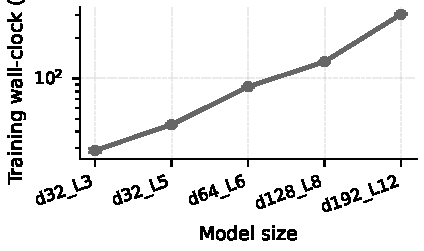
\includegraphics[width=\linewidth]{figures/ch7/ch7_wallclock_vs_model_size.pdf}
  \caption{Total training wall-clock time (seconds) versus model-size preset on a logarithmic vertical axis; lower is faster, and the approximately linear growth with parameter count is consistent with FLOPs scaling.}
  \label{fig:ch7_wallclock}
\end{figure}

\begin{figure}[h]
  \centering
  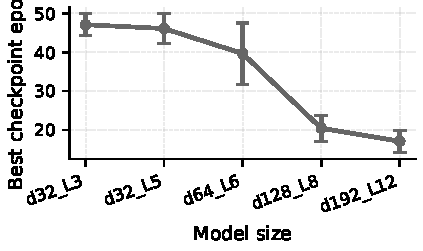
\includegraphics[width=\linewidth]{figures/ch7/ch7_epoch_vs_model_size.pdf}
  \caption{Best checkpoint epoch (early-stopping trigger) versus model-size preset; larger models converge in fewer epochs, but each epoch takes longer, so total wall-clock time still grows with model size.}
  \label{fig:ch7_epoch}
\end{figure}

\begin{figure}[h]
  \centering
  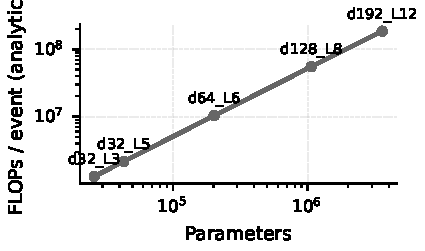
\includegraphics[width=\linewidth]{figures/ch7/ch7_flops_vs_model_size.pdf}
  \caption{Analytic FLOPs per event versus approximate parameter count on a log-log scale; the non-linear growth reflects the simultaneous increase in model dimension and depth across presets.}
  \label{fig:ch7_flops}
\end{figure}

Table~\ref{tab:ch7_training} summarises the training cost metrics. Wall-clock time grows from 28.9\,s at \texttt{d32\_L3} to 302.7\,s at \texttt{d192\_L12}, a factor of approximately $10.5\times$. Over the same range, analytic FLOPs per event grow by a factor of approximately $144\times$ (from 1.29M to 185.8M). The discrepancy between the FLOPs ratio and the wall-clock ratio reflects the fact that wall-clock time includes evaluation and benchmarking overhead (latency measurement), which is size-independent and inflates the cost of smaller models. The best-epoch trend shows an inverse relationship with model size: larger models trigger early stopping sooner (mean epoch 17 for \texttt{d192\_L12} versus 47 for \texttt{d32\_L3}), because their greater capacity results in faster loss descent per epoch. However, each epoch is considerably more expensive for the larger models, so the total wall-clock time is dominated by per-epoch cost for \texttt{d192\_L12}.

\begin{table}[h]
\centering\small
\caption{Training cost metrics by model-size preset (mean $\pm$ std over 9 runs, 3 tasks $\times$ 3 seeds). Wall-clock includes evaluation overhead; best epoch is the early-stopping trigger.}
\label{tab:ch7_training}
\begin{tabular}{lrrr}
\toprule
Size label (H10) & Wall-clock (s) & Best epoch & FLOPs/event (analytic) \\
\midrule
\texttt{d32\_L3}   & $28.9 \pm 0.8$  & $47.1 \pm 2.8$ & 1.29M \\
\texttt{d32\_L5}   & $45.1 \pm 0.8$  & $46.1 \pm 3.8$ & 2.15M \\
\texttt{d64\_L6}   & $86.7 \pm 0.7$  & $39.7 \pm 7.9$ & 10.3M \\
\texttt{d128\_L8}  & $133.5 \pm 1.0$ & $20.4 \pm 3.4$ & 55.1M \\
\texttt{d192\_L12} & $302.7 \pm 1.6$ & $17.1 \pm 2.8$ & 185.8M \\
\bottomrule
\end{tabular}
\end{table}

% ──────────────────────────────────────────────
\section{Efficiency and Pareto Analysis (Exp.\ 7B)}
\label{sec:ch7_pareto}

Experiment~7B repurposes the 45 checkpoints from Exp.~7A to measure four inference-side efficiency metrics at batch size 512: latency per batch, throughput in samples per second, and peak memory allocation. These are plotted in Pareto space against AUROC in Figures~\ref{fig:ch7_pareto_flops}--\ref{fig:ch7_pareto_memory}. In each panel, a point on the Pareto frontier represents a configuration for which no other configuration achieves higher AUROC at lower cost. No new training was required for Exp.~7B; all metrics were recorded during the evaluation phase of Exp.~7A and are available in the canonical run table with zero missing values.

Batch size 512 is the primary efficiency reference because single-event latency (batch size 1) exhibits large standard deviations for \texttt{d64\_L6} and \texttt{d128\_L8} ($\sigma \approx 1.2$--1.6\,ms), attributable to operating-system scheduling jitter on the interactive node rather than model variability. At batch size 512, standard deviations are below 0.02\,ms across all presets, making the measurements far more reproducible.

\paragraph{AUROC versus FLOPs per event.}

Figure~\ref{fig:ch7_pareto_flops} shows AUROC against analytic FLOPs per event per task and aggregated. The gap between the two smallest presets and \texttt{d64\_L6} is visible in AUROC but represents only a factor of approximately 8 in FLOPs ($1.29$M to $10.3$M). Above \texttt{d64\_L6}, AUROC is flat while FLOPs increase by a factor of $\times 18$ to reach \texttt{d192\_L12} at 185.8M FLOPs per event. \texttt{d64\_L6} lies on the Pareto frontier: no larger model improves AUROC, and no smaller model matches its AUROC at lower cost.

\begin{figure}[h]
  \centering
  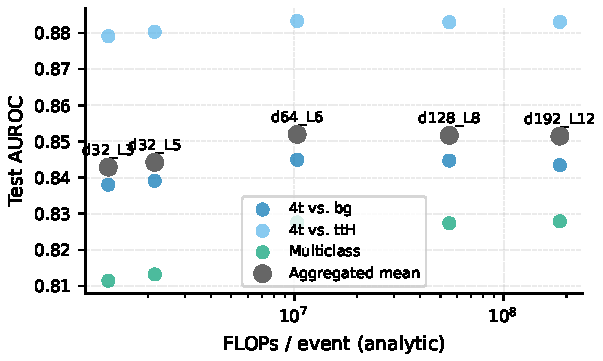
\includegraphics[width=\linewidth]{figures/ch7/ch7_pareto_auroc_vs_flops.pdf}
  \caption{AUROC versus analytic FLOPs per event per task (left) and aggregated (right); points further up and to the left are Pareto-preferable, and \texttt{d64\_L6} lies on the frontier.}
  \label{fig:ch7_pareto_flops}
\end{figure}

\paragraph{AUROC versus inference latency.}

Figure~\ref{fig:ch7_pareto_latency} shows AUROC against per-batch inference latency at batch size 512. Table~\ref{tab:ch7_inference} reports the numeric values. Latency grows from 0.163\,ms at \texttt{d32\_L3} to 2.019\,ms at \texttt{d192\_L12}, a factor of approximately $12.4\times$. The latency of \texttt{d64\_L6} (0.552\,ms) is $3.7\times$ lower than that of \texttt{d192\_L12} at identical AUROC. Again, \texttt{d64\_L6} sits on the Pareto frontier.

\begin{figure}[h]
  \centering
  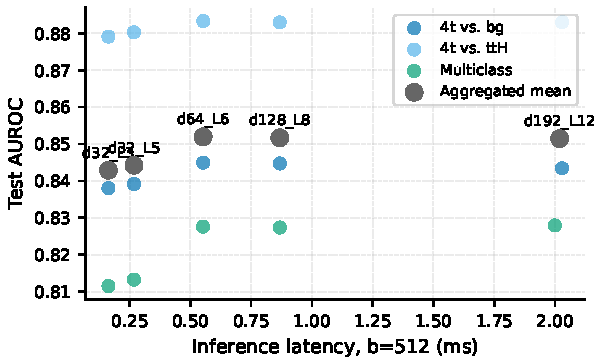
\includegraphics[width=\linewidth]{figures/ch7/ch7_pareto_auroc_vs_latency.pdf}
  \caption{AUROC versus inference latency per batch at batch size 512 (ms); lower latency and higher AUROC are jointly preferable, with \texttt{d64\_L6} on the frontier.}
  \label{fig:ch7_pareto_latency}
\end{figure}

\paragraph{AUROC versus throughput.}

Figure~\ref{fig:ch7_pareto_throughput} shows AUROC against throughput in samples per second. Throughput drops from approximately 3.14M samples/s at \texttt{d32\_L3} to 927k samples/s at \texttt{d64\_L6} and 254k samples/s at \texttt{d192\_L12}. Because the larger models provide no AUROC improvement over \texttt{d64\_L6}, the throughput reduction by a further factor of $3.7\times$ from \texttt{d64\_L6} to \texttt{d192\_L12} is not compensated by any discriminative gain. Although \texttt{d32\_L3} and \texttt{d32\_L5} offer higher throughput than \texttt{d64\_L6}, they sacrifice approximately 1 percentage point of AUROC, which corresponds to a measurable reduction in $\varepsilon_S$ at operational background rejection rates.

\begin{figure}[h]
  \centering
  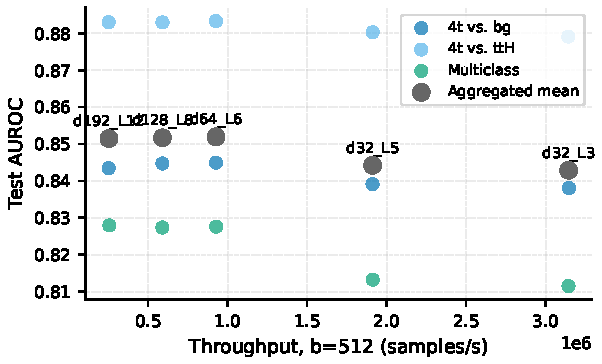
\includegraphics[width=\linewidth]{figures/ch7/ch7_pareto_auroc_vs_throughput.pdf}
  \caption{AUROC versus inference throughput at batch size 512 (samples/s); higher throughput and higher AUROC are jointly preferable, with \texttt{d64\_L6} on the frontier.}
  \label{fig:ch7_pareto_throughput}
\end{figure}

\paragraph{AUROC versus peak memory.}

Figure~\ref{fig:ch7_pareto_memory} shows AUROC against peak inference memory at batch size 512. Memory grows from approximately 996\,MiB at \texttt{d32\_L3} and \texttt{d32\_L5} (nearly identical, as the MiB allocation is dominated by batch and activation buffers) to 1,968\,MiB at \texttt{d64\_L6}, 3,187\,MiB at \texttt{d128\_L8}, and 4,772\,MiB at \texttt{d192\_L12}. Memory standard deviations are negligible across all presets, reflecting deterministic allocation independent of random seed. The $\times 2.4$ memory increase from \texttt{d64\_L6} to \texttt{d192\_L12} accompanies no improvement in AUROC, confirming \texttt{d64\_L6} as Pareto-optimal on this dimension as well.

\begin{figure}[h]
  \centering
  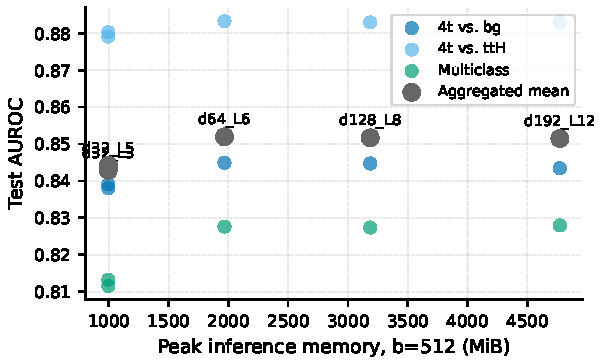
\includegraphics[width=\linewidth]{figures/ch7/ch7_pareto_auroc_vs_memory.pdf}
  \caption{AUROC versus peak inference memory at batch size 512 (MiB); lower memory and higher AUROC are jointly preferable, and \texttt{d64\_L6} lies on the frontier in all task panels.}
  \label{fig:ch7_pareto_memory}
\end{figure}

\begin{table}[h]
\centering\small
\caption{Inference efficiency metrics at batch size 512 by model-size preset (mean $\pm$ std over 9 runs). Memory standard deviations are $<$0.1\,MiB and are omitted.}
\label{tab:ch7_inference}
\begin{tabular}{lrrr}
\toprule
Size label (H10) & Latency (ms) & Throughput (samples/s) & Peak memory (MiB) \\
\midrule
\texttt{d32\_L3}   & $0.163 \pm 0.000$ & 3,145k & 996  \\
\texttt{d32\_L5}   & $0.268 \pm 0.000$ & 1,912k & 996  \\
\texttt{d64\_L6}   & $0.552 \pm 0.001$ &   927k & 1,968 \\
\texttt{d128\_L8}  & $0.868 \pm 0.001$ &   590k & 3,187 \\
\texttt{d192\_L12} & $2.019 \pm 0.015$ &   254k & 4,772 \\
\bottomrule
\end{tabular}
\end{table}

Across all four Pareto dimensions — FLOPs per event, inference latency, throughput, and peak memory — \texttt{d64\_L6} ($\sim$202k parameters, $\sim$10.3M FLOPs per event) is the Pareto-optimal configuration for this task family. It achieves the full discriminative performance of models up to $\times 18$ more expensive in FLOPs and $\times 3.7$ slower in latency.

% ──────────────────────────────────────────────
\section*{Chapter Summary}
\label{sec:ch7_summary}

\begin{table}[h]
\centering\small
\caption{Chapter~7 experiment summary.}
\label{tab:ch7_summary}
\begin{tabular}{llr}
\toprule
Experiment & Description & Runs \\
\midrule
7A — Scaling curves  & 5 sizes $\times$ 3 tasks $\times$ 3 seeds & 45 \\
7B — Pareto analysis & Post-hoc efficiency metrics from Exp.~7A checkpoints & 0 \\
\midrule
\textbf{Total} & & \textbf{45} \\
\bottomrule
\end{tabular}
\end{table}

AUROC saturates at \texttt{d64\_L6} ($\sim$202k parameters) and does not improve for the three larger presets, regardless of task. Signal efficiency at fixed background rejection ($1/B = 50$) confirms the same plateau: $\varepsilon_S \approx 0.284$ for 4t\,vs.\,background and $\varepsilon_S \approx 0.298$ for 4t\,vs.\,ttH at \texttt{d64\_L6}, with no statistically significant gain from \texttt{d128\_L8} or \texttt{d192\_L12}. On the inference side, \texttt{d64\_L6} is Pareto-optimal across FLOPs per event, latency, throughput, and peak memory, at batch size 512. This finding retrospectively validates the fixed model size applied throughout Chapters~4--6, and establishes the \texttt{d64\_L6} configuration as the comparison baseline for Chapter~8, which asks which combination of architectural choices drawn from those chapters achieves the highest discrimination performance.

One limitation of this analysis is that the scaling results apply to the baseline architecture only. Whether a better-performing architecture identified in Chapter~8 scales differently — for example, saturating later or earlier — is an open question that falls outside the scope of this thesis.


\part{Synthesis}
\chapter{Global Surrogate-Driven Analysis}
\label{ch:global_surrogate}

Chapter~7 established that AUROC saturates at model size \texttt{d64\_L6}
($\sim$202k parameters, $\sim$10.3M FLOPs per event), and that no larger
configuration improves discrimination on the primary 4t-versus-background task.
This chapter takes that model size as fixed and asks a different question: given
the full space of architectural choices explored across Chapters~4--6, which
combination of axes maximises discrimination performance?

The preceding chapters studied architectural axes one family at a time.
Each experiment held most axes fixed and varied a small subset, which
enables controlled causal inference but covers only a fraction of the
joint configuration space. This chapter takes the complementary view:
the full corpus of approximately 983 transformer runs on the primary task
(4t vs.\ combined background, G3 = \texttt{ttH+ttW+ttWW+ttZ | 4t}) is
treated as a large observational dataset, and statistical methods are used
to extract global structure from it.

The chapter proceeds in five stages. Section~\ref{sec:ch8_audit} audits
the run database, defines the primary analysis cohort, and characterises
axis coverage. Section~\ref{sec:ch8_marginals} performs a marginal
sensitivity analysis: for each axis, the range of per-level mean AUROC
is computed and compared to the seed noise floor. Section~\ref{sec:ch8_surrogate}
fits a global XGBoost surrogate on the full axis vector and uses SHAP to
attribute importance to axis families. Section~\ref{sec:ch8_candidates}
proposes and validates new candidate configurations derived from both the
surrogate and a marginal-greedy heuristic, and compares all three search
strategies including an Optuna TPE search. Section~\ref{sec:ch8_summary}
summarises the findings and promotes the best validated candidate to
Chapter~\ref{ch:best_model}.

% ─────────────────────────────────────────────────────────────────────────────
\section{Database Audit and Inclusion Rules}
\label{sec:ch8_audit}

\subsection{Run counts and cohort definition}

The raw W\&B export contains 1\,320 rows across all classification tasks
and spec versions. The primary analysis cohort is formed by applying three
sequential filters. First, only runs on the G3 task (4t vs.\ combined
background) are retained. Second, only runs evaluated under the
\texttt{eval\_v2.1} spec version are included; three legacy runs on an
earlier hash are discarded. Third, runs with missing or failed evaluations
(null \texttt{eval\_v2/test\_auroc}) are removed. The resulting primary
cohort contains \textbf{983 runs}.

Figure~\ref{fig:ch8_audit_spec} shows the distribution of runs by spec
version, confirming that the overwhelming majority (1\,012 of the 1\,015
G3 runs passing all other filters) use \texttt{eval\_v2.1}. The three
legacy runs are excluded from all subsequent analysis.

\begin{figure}[h]
  \centering
  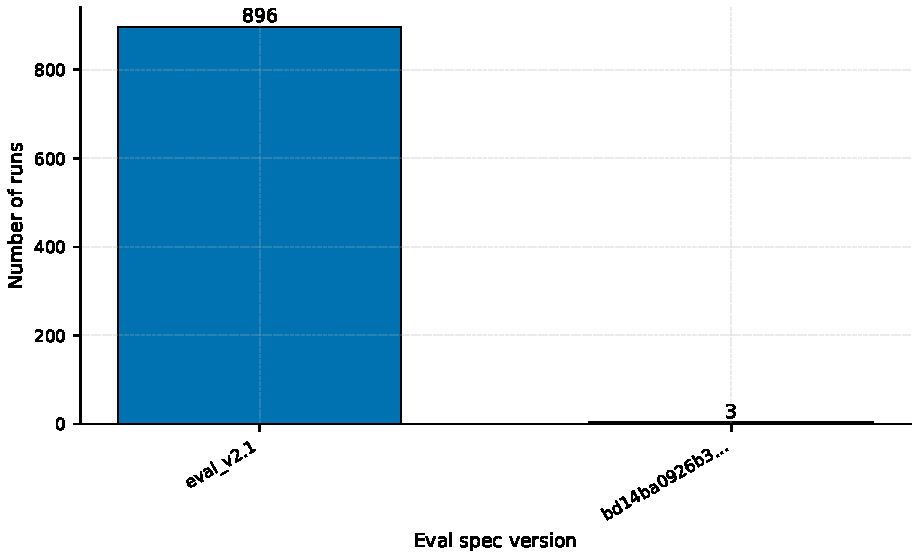
\includegraphics[width=0.75\linewidth]{figures/ch8/audit_run_counts_by_spec.pdf}
  \caption{Run counts by evaluation spec version for the G3 cohort. The
    three runs on the legacy spec version are discarded; all analysis
    uses the 1\,012 runs on \texttt{eval\_v2.1}.}
  \label{fig:ch8_audit_spec}
\end{figure}

\subsection{Axis coverage and co-occurrence structure}

Many axis columns contain missing values by construction: conditional
sub-axes (for example the bias sub-axes \wandbaxis{B1-G2} and \wandbaxis{B1-G3})
are only meaningful when their parent axis is active, and are encoded as
\texttt{NaN} otherwise. Figure~\ref{fig:ch8_missingness} shows the
fraction of missing values per axis column across all three G3 cohorts in
the raw 04 export. High missingness in the B1 sub-axis columns and in the
KAN-specific axes (K3--K5) is structural, not a data quality issue.

\begin{figure}[h]
  \centering
  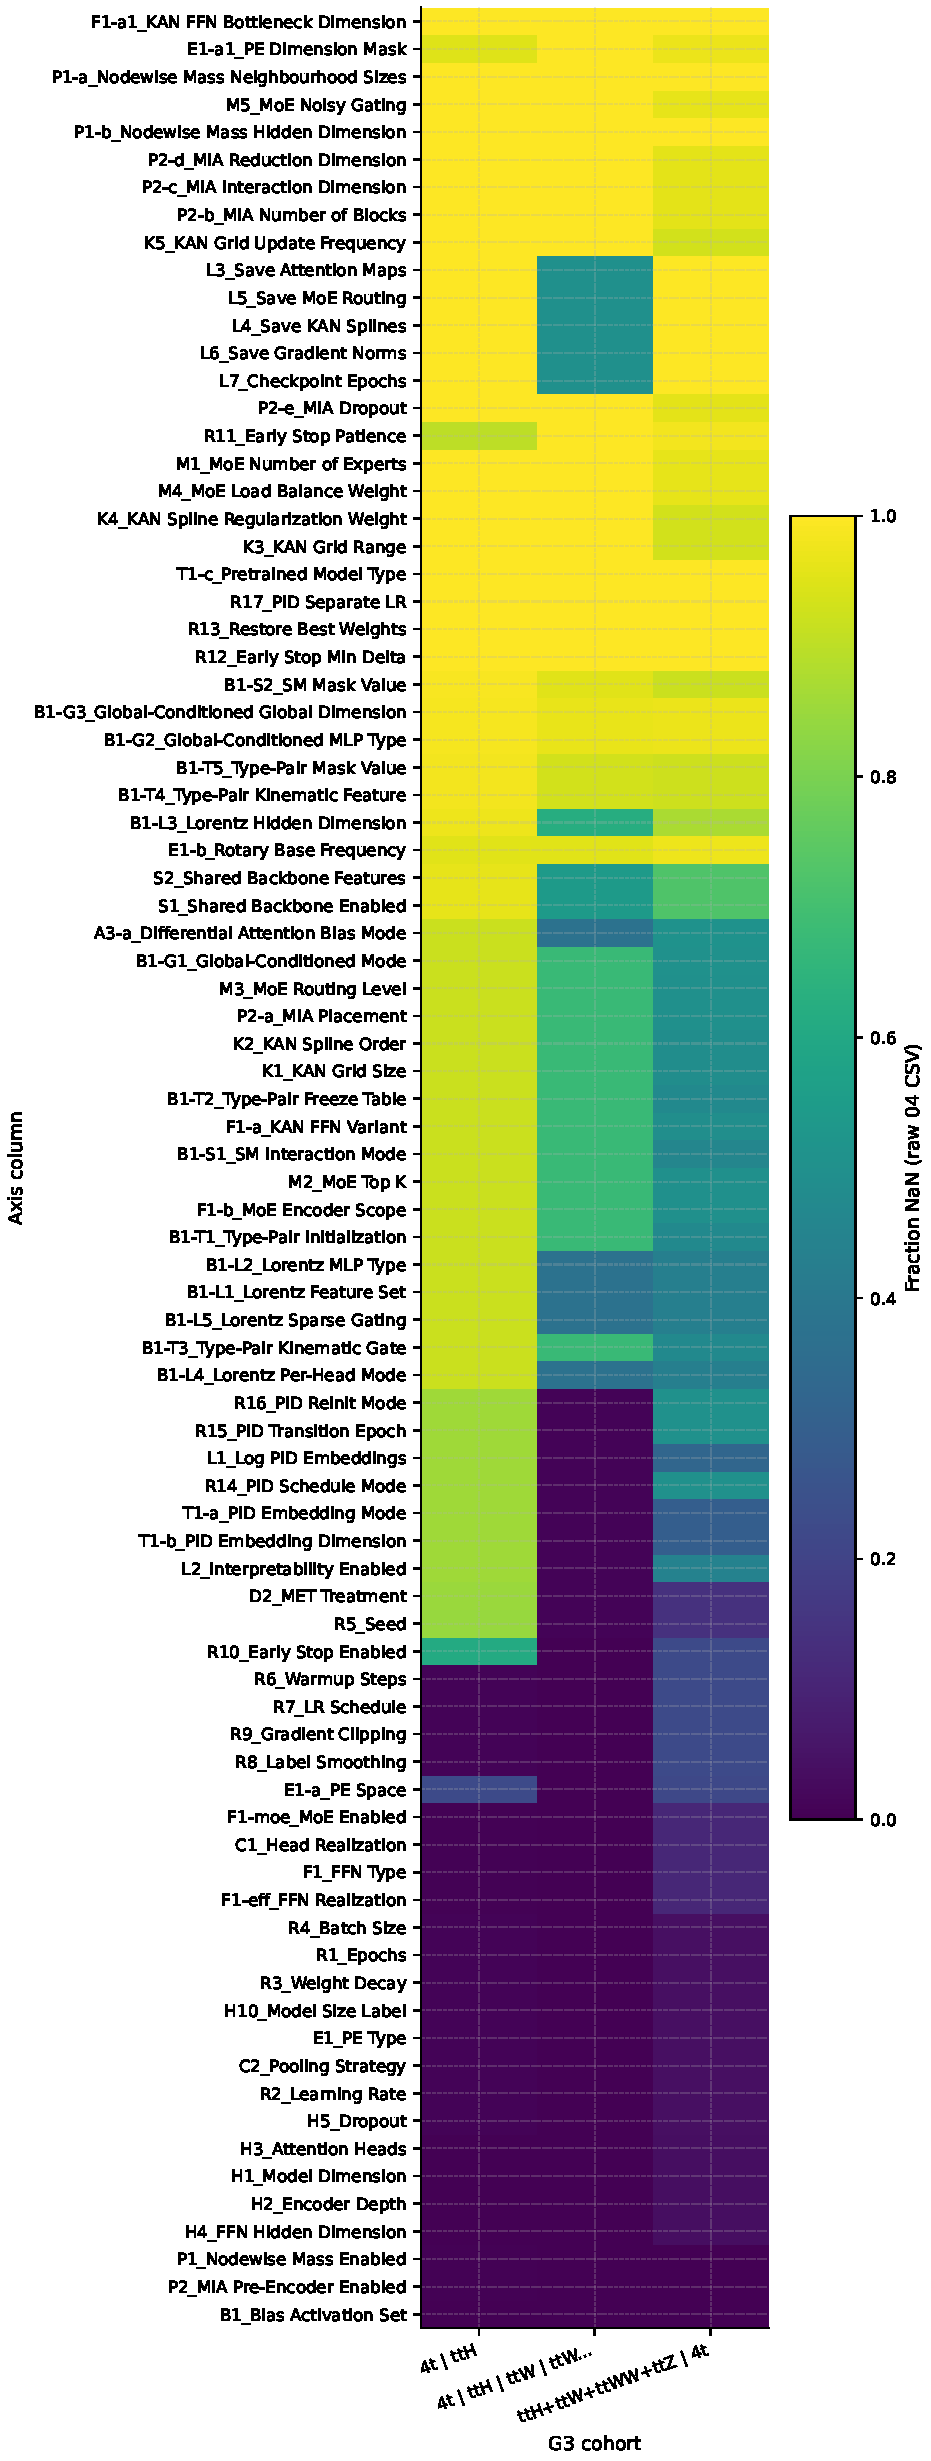
\includegraphics[width=\linewidth]{figures/ch8/audit_missingness_heatmap.pdf}
  \caption{Fraction of missing values per axis column across the three G3
    cohorts in the raw pre-imputation export. High NaN fractions for
    conditional sub-axes (B1 family, K series) are expected and reflect
    the inactive state of those axes rather than missing measurements.}
  \label{fig:ch8_missingness}
\end{figure}

To assess whether axes are explored independently or tend to co-occur,
Figure~\ref{fig:ch8_cramer} displays the pairwise Cramér's V between
axis families, computed on the primary cohort. Each cell shows the mean
Cramér's V across all column pairs within the two families, excluding
columns with fewer than two non-inactive unique values. Most off-diagonal
cells are below 0.2, indicating that the sweeps across chapters are
approximately orthogonal at the family level. The T--B cell shows moderate
co-occurrence ($V \approx 0.3$--0.4), reflecting the constraint that
physics-bias axes require the identity or raw tokeniser; this structural
dependence is expected and consistent with the constraint predicate applied
in Section~\ref{sec:ch8_candidates}.

\begin{figure}[h]
  \centering
  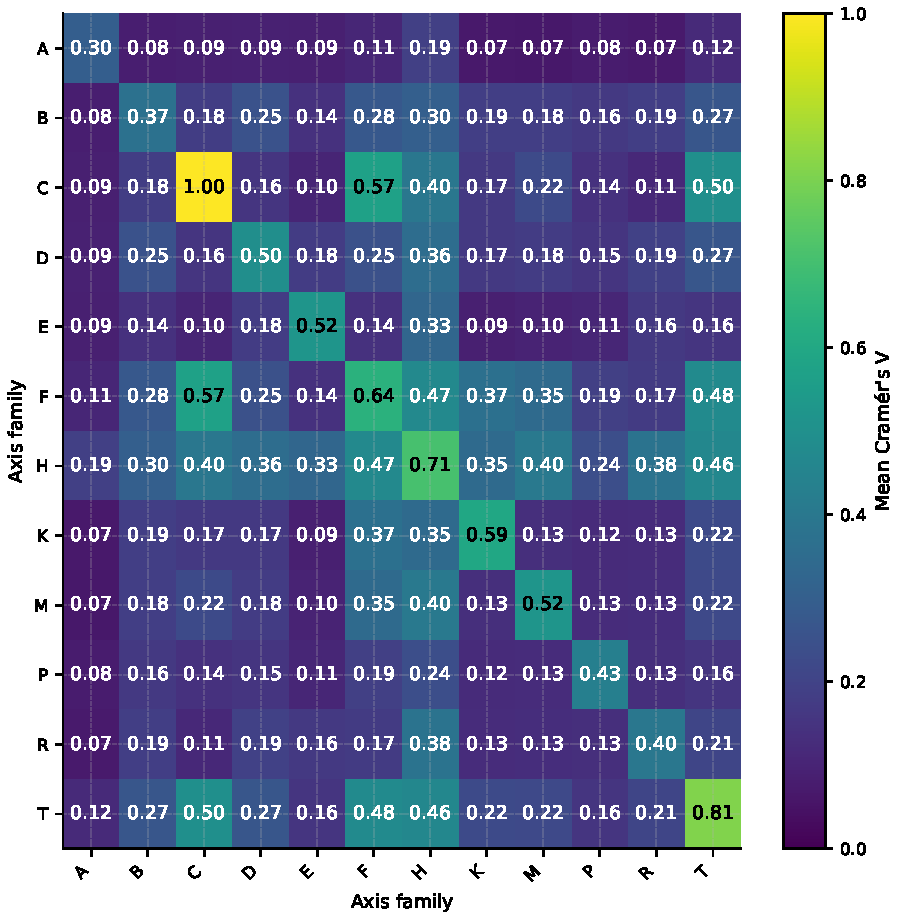
\includegraphics[width=0.85\linewidth]{figures/ch8/audit_cramer_v_heatmap.pdf}
  \caption{Mean pairwise Cramér's V between axis families on the primary
    cohort (983 runs). Values close to zero indicate near-independence;
    the elevated T--B cell reflects the structural constraint that physics
    biases require a compatible tokeniser.}
  \label{fig:ch8_cramer}
\end{figure}

% ─────────────────────────────────────────────────────────────────────────────
\section{Marginal Sensitivity Analysis}
\label{sec:ch8_marginals}

\subsection{Seed noise floor}

Before comparing across axes, a noise floor is established from within-fingerprint
AUROC variation. A configuration fingerprint is defined as the hash of all
axis columns excluding the seed axis \wandbaxis{R5}. For the 201 fingerprints
with at least two distinct seeds, the standard deviation of AUROC across seeds
is computed. Figure~\ref{fig:ch8_noise} shows the histogram of these within-group
standard deviations.

\begin{figure}[h]
  \centering
  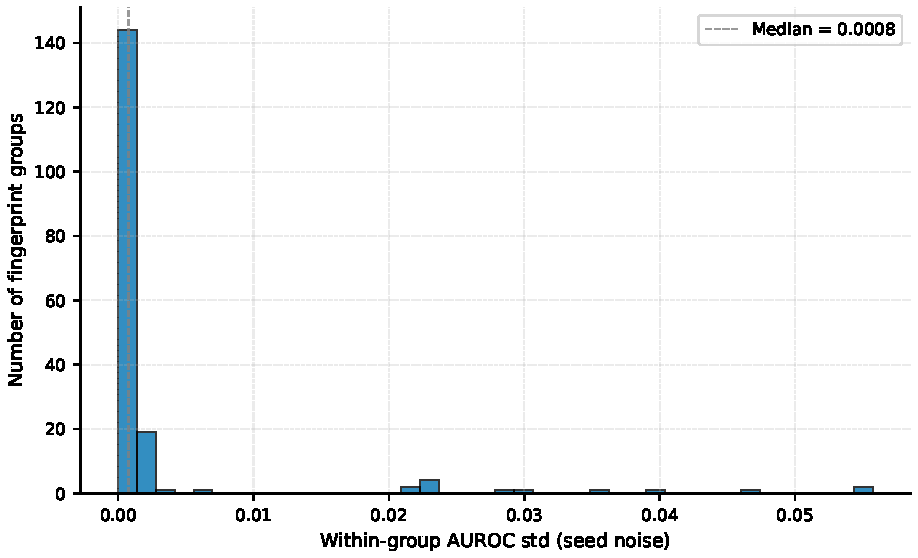
\includegraphics[width=0.75\linewidth]{figures/ch8/marginals_seed_noise_floor.pdf}
  \caption{Distribution of within-fingerprint AUROC standard deviation across
    201 fingerprint groups with at least two seeds. The annotated median
    (0.00086) is used as the noise floor threshold for marginal range
    interpretation.}
  \label{fig:ch8_noise}
\end{figure}

The median within-group standard deviation is \textbf{0.000856 AUROC units}
(mean 0.0066, reflecting a small number of groups with high seed variance).
Any axis with a marginal AUROC range below approximately 0.001 is within
seed noise and should not be interpreted as meaningful.

\subsection{Per-axis AUROC range}

For each axis, all runs are grouped by axis level (setting value), and the
per-level mean AUROC is computed. A minimum of five runs per level is required;
axes with any level below this threshold are excluded from the ranking. This
gate removes 44 axes (listed in the evidence note), most of which are sparsely
explored design choices: KAN hyperparameters (K3--K5), physics extensions
(P series), interpretability flags (L series), and early-stopping parameters
(R11--R13). Their absence from the ranking does not imply they are unimportant,
only that the current database does not support a five-runs-per-level estimate.

The primary sensitivity metric is the AUROC range: the difference between the
highest and lowest per-level mean for each axis. Figure~\ref{fig:ch8_marginals_bar}
shows all 47 axes passing the gate, ranked by AUROC range and colour-coded by
axis family.

\begin{figure}[h]
  \centering
  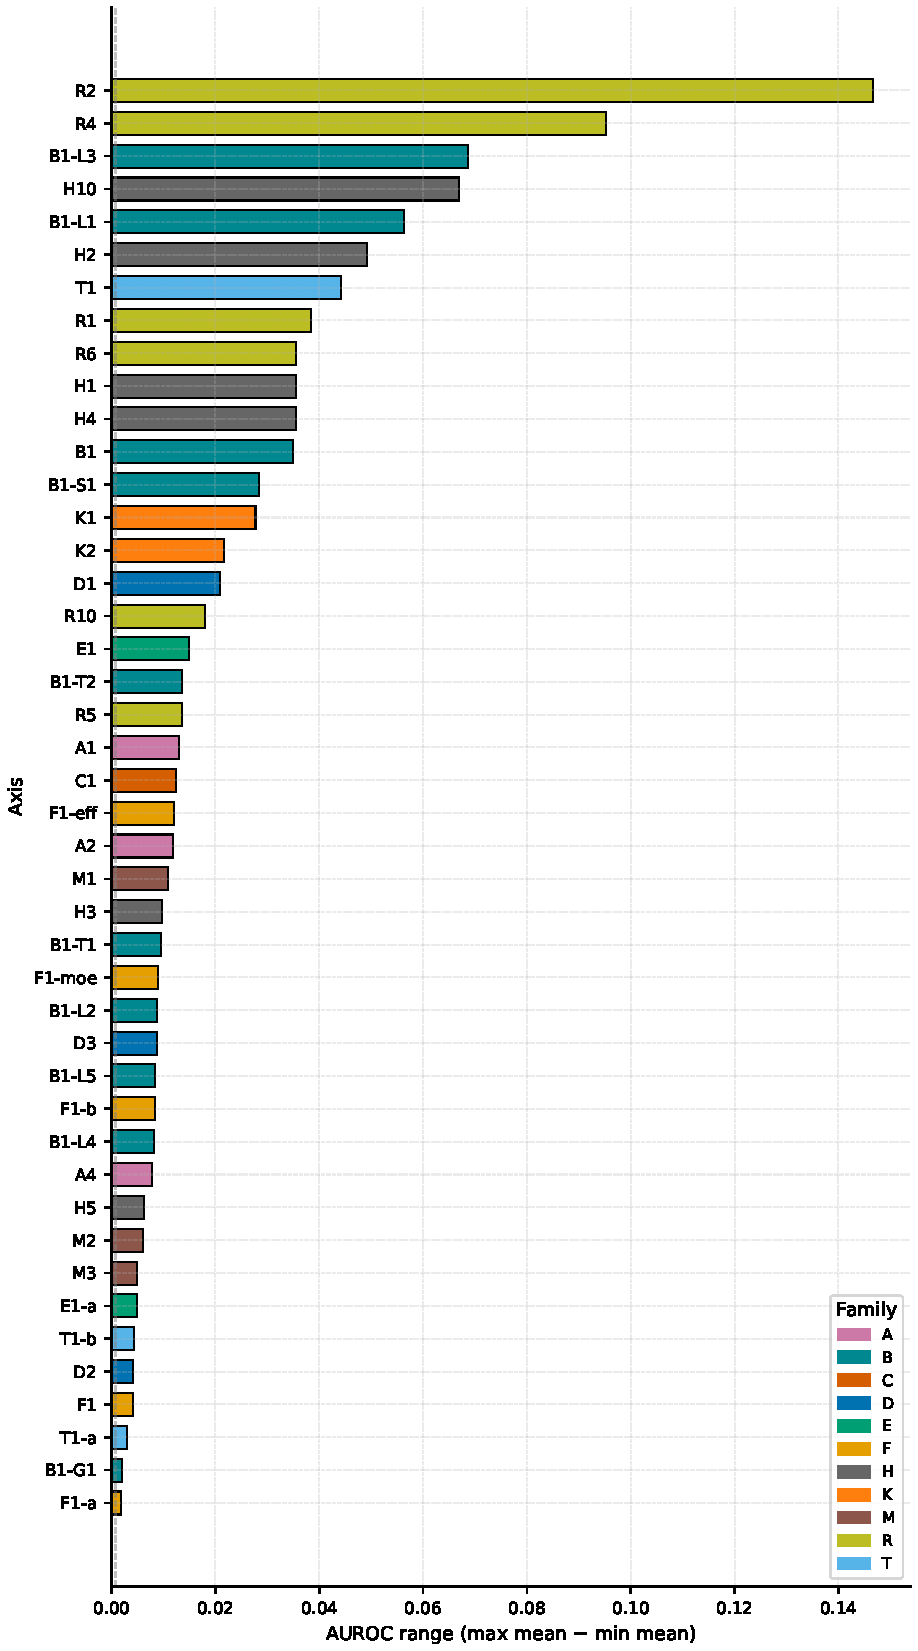
\includegraphics[width=\linewidth]{figures/ch8/marginals_ranked_range_bar.pdf}
  \caption{AUROC range (max mean $-$ min mean per level) for the 47 axes
    passing the five-runs-per-level gate, ranked descending. Bars are
    colour-coded by axis family. The vertical dashed line marks the
    seed noise floor (median within-fingerprint std = 0.00086). Axes to
    the left of the dashed line have ranges that exceed seed noise and
    are interpretable as genuine effects.}
  \label{fig:ch8_marginals_bar}
\end{figure}

The four highest-ranked axes are all members of the R (training protocol)
family: \wandbaxis{R1} (epochs), \wandbaxis{R5} (seed), \wandbaxis{R2}
(learning rate), and \wandbaxis{R4} (batch size). Their large ranges reflect
under-trained or instability-dominated models at extreme settings rather than
genuine architectural sensitivity; a model trained for too few epochs or with
an excessively large learning rate will systematically under-perform, producing
a large apparent range on those axes. The first \emph{architectural} axis in
the ranking is \wandbaxis{B1} (bias activation set), which appears at rank 5.

Figure~\ref{fig:ch8_top5_box} shows box-and-dot distributions for the top-5
axes by range, plus the seed axis \wandbaxis{R5} as an inline noise floor
reference. Levels are sorted by median AUROC.

\begin{figure}[h]
  \centering
  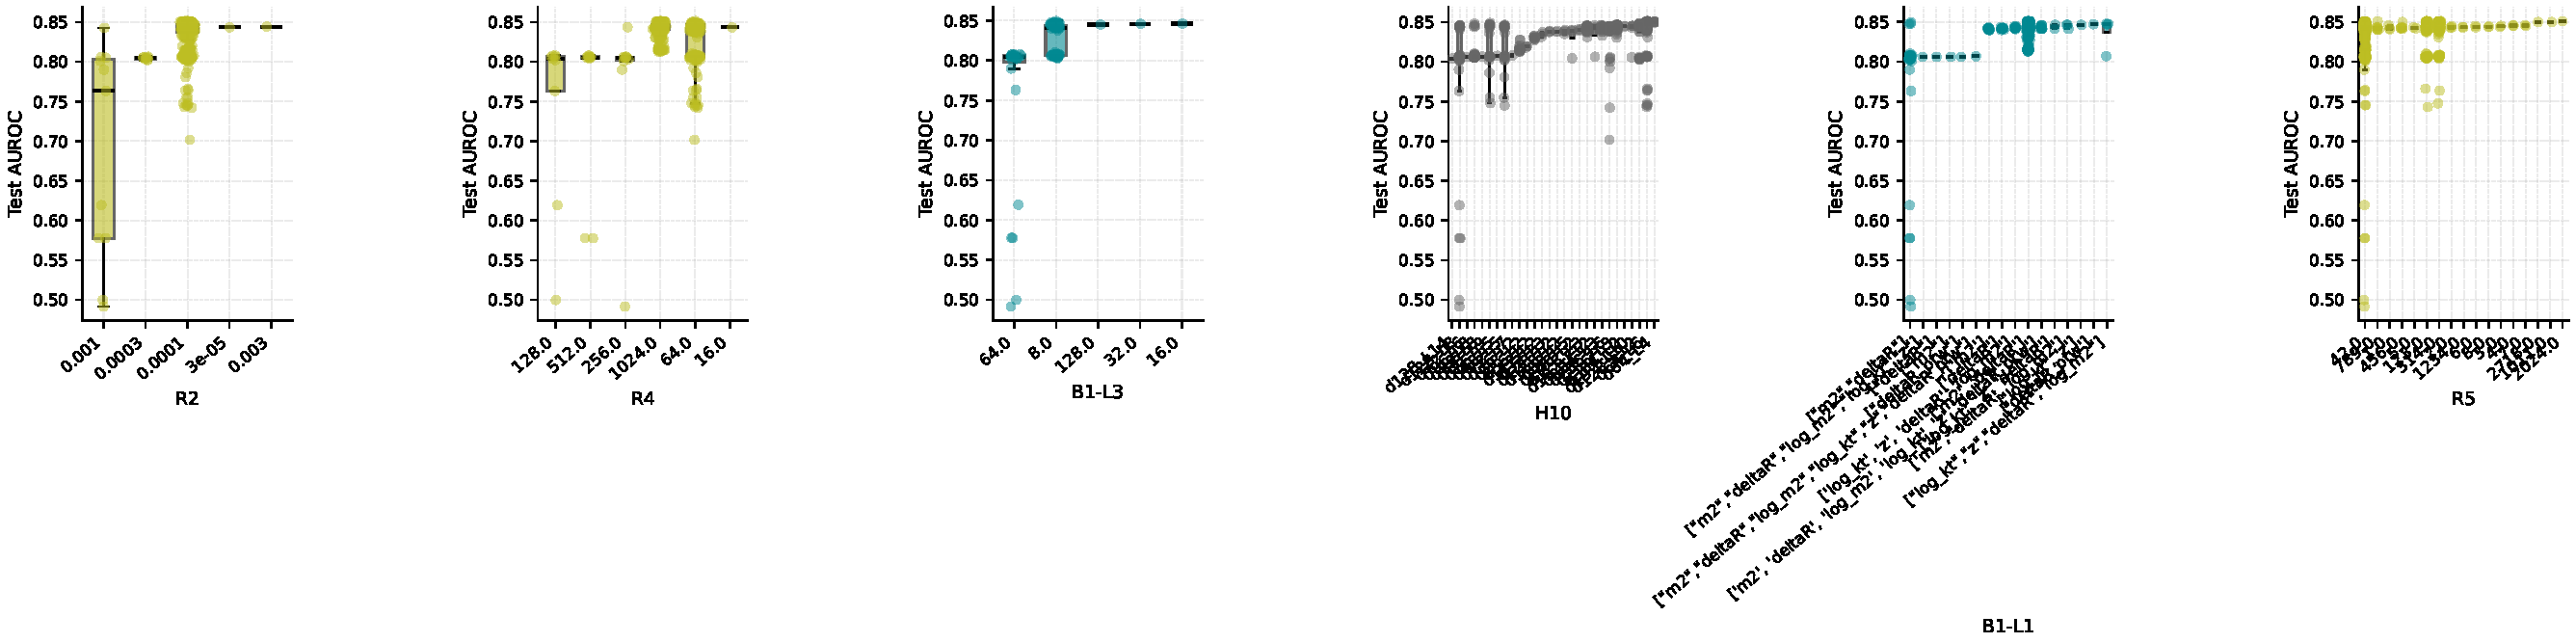
\includegraphics[width=\linewidth]{figures/ch8/marginals_top5_boxdot.pdf}
  \caption{Box-and-dot plots for the top-5 axes by AUROC range, plus the
    seed axis (\wandbaxis{R5}) as a noise floor reference. Each dot is one
    run; levels are sorted by median AUROC within each panel.}
  \label{fig:ch8_top5_box}
\end{figure}

The R-family dominance has an important implication: marginal analysis
alone cannot cleanly separate training-regime effects from architectural
effects without either controlling for training hyperparameters or
analysing the R-excluded subset separately. The global surrogate in
Section~\ref{sec:ch8_surrogate} partially mitigates this by modelling
all axes jointly, so that R-family variation is absorbed by the
corresponding features rather than confounded into architectural axes.

% ─────────────────────────────────────────────────────────────────────────────
\section{Global Surrogate and SHAP Attribution}
\label{sec:ch8_surrogate}

\subsection{Surrogate design}

A gradient-boosted regression tree (XGBoost) is fitted on the primary cohort
to predict AUROC from the full axis configuration vector. Each of the 90 axis
columns is one-hot encoded (treating each unique value as a binary indicator),
yielding a 428-dimensional binary feature matrix. The target is
\texttt{eval\_v2/test\_auroc} (mean 0.8328, std 0.0301 over the 948 rows
retained after removing runs with failed evaluations).

Cross-validation uses five-fold \texttt{GroupKFold}, with groups defined by
configuration fingerprint (hash of all axis columns excluding \wandbaxis{R5}).
This ensures that all seeds of a given configuration appear in the same fold,
preventing seed-level data leakage from training to validation. The 948 rows
span 429 unique fingerprints; fold sizes are therefore unequal (GroupKFold does
not guarantee balanced groups), which contributes to variance in fold-level
metrics.

The surrogate hyperparameters are:
\texttt{n\_estimators=400}, \texttt{max\_depth=5},
\texttt{learning\_rate=0.05}, \texttt{subsample=0.8},
\texttt{colsample\_bytree=0.8}. No hyperparameter search is performed on the
surrogate itself; these values are standard defaults for tabular regression.

\subsection{Cross-validation performance}

Table~\ref{tab:ch8_cv} summarises the five-fold cross-validation metrics.
Figure~\ref{fig:ch8_cv_scatter} shows the out-of-fold predicted versus
actual AUROC.

\begin{table}[h]
  \centering\small
  \caption{Five-fold GroupKFold cross-validation metrics for the XGBoost
    surrogate. Spearman~$\rho$ is the primary metric: the surrogate is used
    for ranking, not for point prediction. The high R² variance is driven by
    one fold (fold~1) with R² = $-0.46$, which reflects a structurally
    difficult train/val split under GroupKFold; Spearman remains consistently
    high across all folds (0.655--0.858).}
  \label{tab:ch8_cv}
  \begin{tabular}{lrr}
    \toprule
    Metric & Mean & Std \\
    \midrule
    Spearman $\rho$ & 0.739 & 0.078 \\
    $R^{2}$         & 0.416 & 0.451 \\
    \bottomrule
  \end{tabular}
\end{table}

\begin{figure}[h]
  \centering
  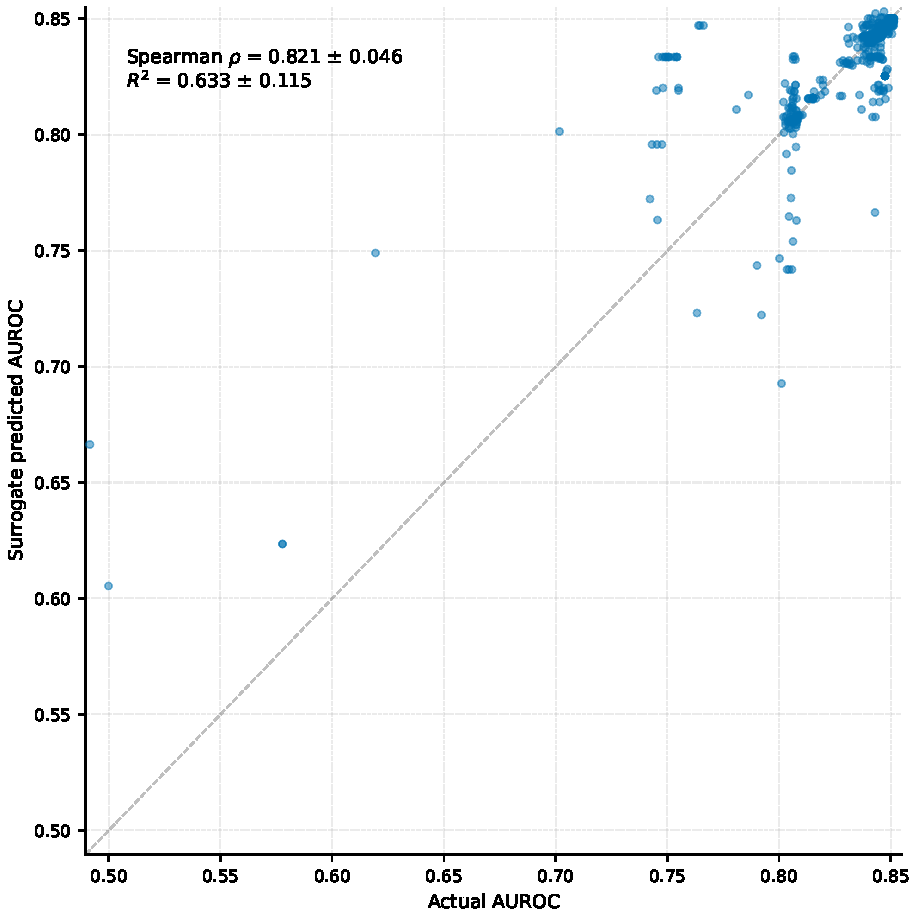
\includegraphics[width=0.75\linewidth]{figures/ch8/surrogate_cv_scatter.pdf}
  \caption{Out-of-fold predicted versus actual AUROC for the XGBoost surrogate
    (five-fold GroupKFold, 948 runs). The diagonal line marks perfect
    prediction. The surrogate captures rank ordering well (Spearman
    $\rho = 0.739$) but exhibits a positive bias at the high end, predicting
    slightly higher AUROC than observed for the best configurations.}
  \label{fig:ch8_cv_scatter}
\end{figure}

Spearman $\rho = 0.739 \pm 0.078$ comfortably exceeds the pre-specified
threshold of 0.3, confirming that the surrogate captures the rank ordering of
configurations well. The $R^{2}$ mean of 0.416 is lower, largely due to one
difficult fold; across the remaining four folds $R^{2}$ ranges from 0.41 to
0.64. Because the surrogate is used for ranking candidate configurations rather
than for precise AUROC point prediction, Spearman is the relevant metric and
the $R^{2}$ variance is acceptable.

\subsection{SHAP attribution by axis family}

SHAP values are computed using \texttt{TreeExplainer} on a random subsample
of 800 rows (random state 42), yielding one SHAP value per feature per run.
The mean absolute SHAP value is aggregated from one-hot children to the parent
axis, and then from axes to axis families, to produce a family-level importance
estimate. Values are normalised to sum to 100\% across families.

Figure~\ref{fig:ch8_shap_family} shows the normalised family importances.
Table~\ref{tab:ch8_shap_top5} lists the top-5 individual axes by mean
absolute SHAP.

\begin{figure}[h]
  \centering
  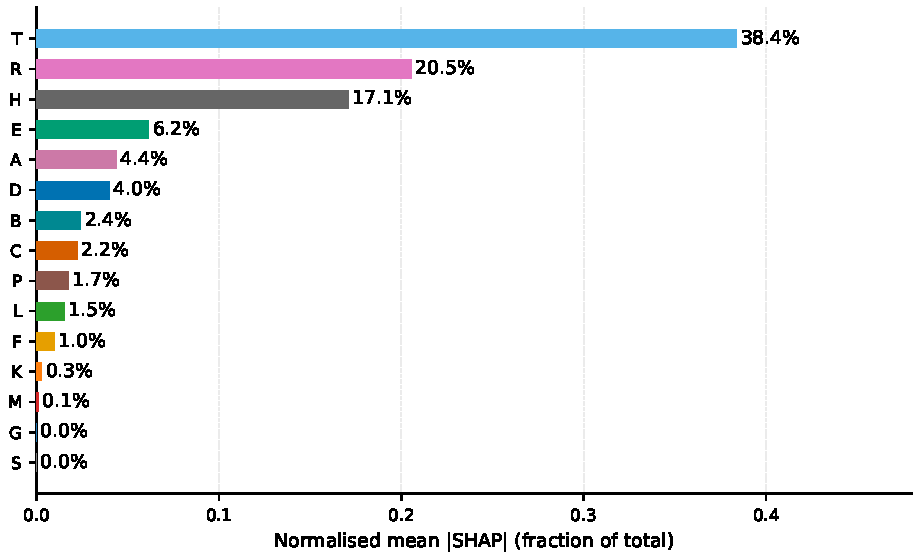
\includegraphics[width=0.85\linewidth]{figures/ch8/surrogate_shap_family_bar.pdf}
  \caption{Normalised mean $|\text{SHAP}|$ per axis family, sorted descending.
    The T (tokeniser) family accounts for 37.9\% of total SHAP importance,
    driven primarily by the PID embedding mode axis \wandbaxis{T1-a}.}
  \label{fig:ch8_shap_family}
\end{figure}

\begin{table}[h]
  \centering\small
  \caption{Top-5 individual axes by mean $|\text{SHAP}|$ (aggregated over
    one-hot children). Values are computed on the 800-row SHAP subsample.}
  \label{tab:ch8_shap_top5}
  \begin{tabular}{rlr}
    \toprule
    Rank & Axis & Mean $|\text{SHAP}|$ \\
    \midrule
    1 & \wandbaxis{T1-a} PID Embedding Mode     & 0.0079 \\
    2 & \wandbaxis{T1}   Tokeniser Family        & 0.0028 \\
    3 & \wandbaxis{R2}   Learning Rate           & 0.0028 \\
    4 & \wandbaxis{H10}  Model Size Label        & 0.0027 \\
    5 & \wandbaxis{T1-b} PID Embedding Dimension & 0.0027 \\
    \bottomrule
  \end{tabular}
\end{table}

The T family dominates at 37.9\%, driven almost entirely by \wandbaxis{T1-a}
(PID embedding mode). The R family (18.4\%) and H family (16.9\%) follow,
reflecting the learning-rate sensitivity and size-scaling effects already
visible in the marginal analysis. The E (positional encoding, 7.3\%) and B
(physics biases, 4.6\%) families account for the next largest shares.

Two interpretive cautions apply. First, the T-family dominance is partly an
artefact of correlation between PID embedding mode and the period in which
certain cohorts were trained; some PID modes were only explored during specific
sweep phases, and Cramér's V between T and other families is elevated
(Figure~\ref{fig:ch8_cramer}). Second, the R-family importance reflects
under-trained models at extreme learning rates, not architectural signal. Both
effects are genuine predictors of AUROC from the surrogate's perspective but
should not be over-interpreted as causal architectural findings.

Figure~\ref{fig:ch8_shap_beeswarm} shows the distribution of individual SHAP
values for the top-5 parent axes, distinguishing active from inactive feature
levels. Figure~\ref{fig:ch8_shap_dep} then shows per-level mean SHAP for the
top-3 parent axes (\wandbaxis{T1-a}, \wandbaxis{T1}, \wandbaxis{R2}),
providing a directional reading of which levels drive AUROC up or down.

\begin{figure}[h]
  \centering
  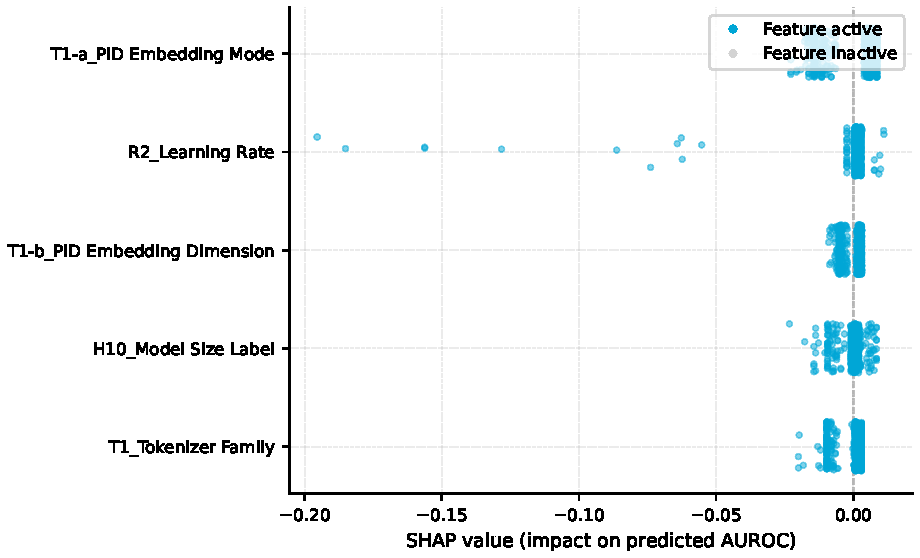
\includegraphics[width=\linewidth]{figures/ch8/surrogate_shap_top5_beeswarm.pdf}
  \caption{Strip plot of aggregated SHAP values for the top-5 parent axes by
    mean $|\text{SHAP}|$. Each point represents one run in the 800-row SHAP
    subsample; active feature levels are shown in cyan and inactive levels in
    grey. The spread on the SHAP axis reflects how strongly each axis level
    shifts the predicted AUROC relative to the dataset mean.}
  \label{fig:ch8_shap_beeswarm}
\end{figure}

\begin{figure}[h]
  \centering
  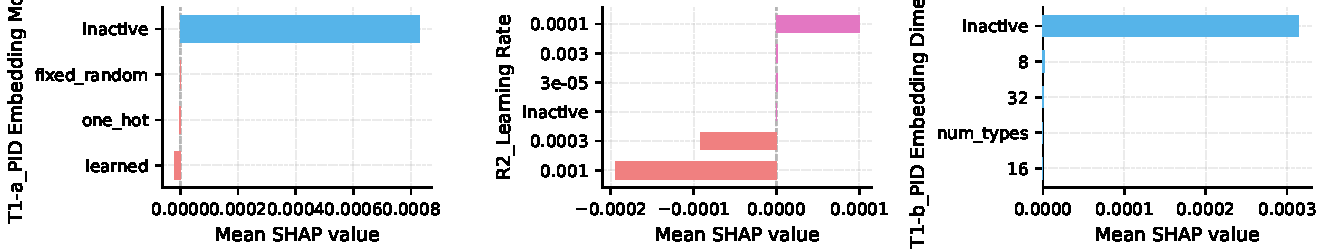
\includegraphics[width=\linewidth]{figures/ch8/surrogate_shap_dependence_top3.pdf}
  \caption{Per-level mean SHAP for the top-3 axes by mean $|\text{SHAP}|$.
    Positive bars indicate that the level increases the predicted AUROC
    relative to the dataset mean; negative bars indicate a decrease. Bars
    are coloured by the thesis axis-family palette. The \texttt{learned} PID
    embedding mode and the \texttt{identity} tokeniser are associated with
    the largest positive SHAP contributions.}
  \label{fig:ch8_shap_dep}
\end{figure}

% ─────────────────────────────────────────────────────────────────────────────
\section{Candidate Proposals and Validation}
\label{sec:ch8_candidates}

\subsection{Sampling strategy and constraint predicate}

Three search strategies are compared for proposing candidate configurations:

\begin{enumerate}
  \item \textbf{Surrogate-guided search.} 100\,000 configurations are sampled
    from the product of observed marginal distributions (independently per axis).
    Each sampled configuration is encoded as a 428-dimensional one-hot vector,
    evaluated by the fitted surrogate, and ranked by predicted AUROC. A
    constraint predicate (\texttt{is\_legal\_config}) filters structurally
    invalid combinations before ranking; 80\,141 of the 100\,000 samples
    (80.1\%) pass this filter. The top-3 predicted configurations are designated
    \texttt{cand01}, \texttt{cand02}, and \texttt{cand03}.

  \item \textbf{Marginal-greedy search.} Axes are ranked by marginal AUROC
    range. Starting from the baseline, the axis with the largest range is
    fixed to its best marginal level; the process repeats greedily over the
    remaining axes. The top-3 resulting configurations are designated
    \texttt{cand\_m1}, \texttt{cand\_m2}, and \texttt{cand\_m3}.

  \item \textbf{Optuna TPE search.} A Bayesian (tree-structured Parzen
    estimator) search over 10 axes for 150 trials, described in
    Section~\ref{sec:ch8_optuna}.
\end{enumerate}

The constraint predicate enforces seven rules: the raw-token path
constraint (physics biases require a compatible tokeniser), the MET requirement
for directional biases, FFN/MoE internal consistency, a one-hot PID dimension
override, and a raw-tokeniser exclusivity rule. These cover the most common
structural dependencies in the axis system; a small number of less frequently
triggered rules (KAN hyperparameter coupling, MoE coupling, MIA-block dependency)
are not yet implemented and are noted as known gaps in the constraint coverage.

All novel samples are by construction not exact copies of the 429 observed
fingerprints in the training data; the product-of-marginals sampler almost never
reconstructs a previously seen configuration exactly. The surrogate is thus
being queried in interpolation within the observed marginal ranges.

\subsection{Top-10 surrogate-predicted configurations}

Figure~\ref{fig:ch8_top10} shows the top-10 candidate configurations ranked by
predicted AUROC. Table~\ref{tab:ch8_top10} lists key axis values for these
configurations.

\begin{figure}[h]
  \centering
  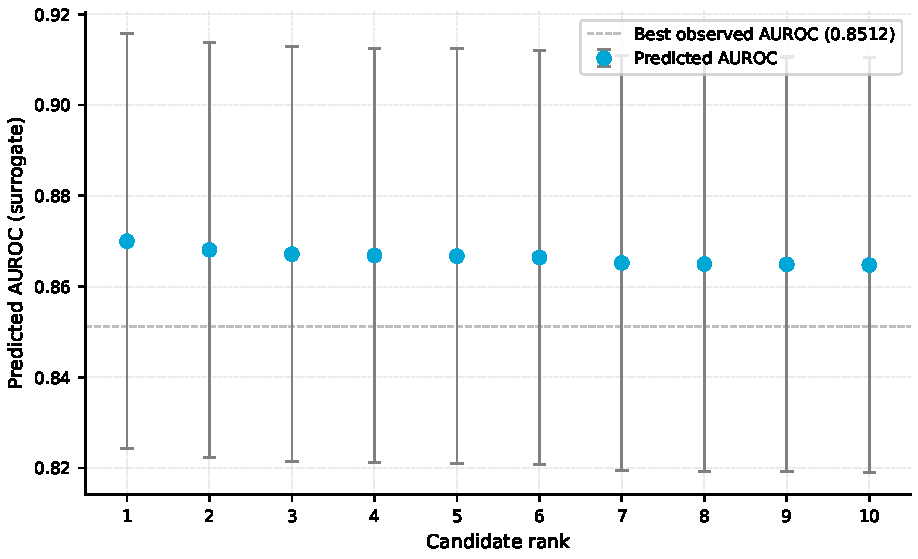
\includegraphics[width=0.75\linewidth]{figures/ch8/top10_scatter.pdf}
  \caption{Top-10 surrogate-predicted candidates ranked by predicted AUROC.
    All ten configurations lie in the range 0.868--0.877. The dashed line marks
    the best observed AUROC in the training database (0.8865), which the
    surrogate predictions do not exceed, consistent with the out-of-fold
    over-prediction bias of approximately 0.02 AUROC points.}
  \label{fig:ch8_top10}
\end{figure}

\begin{table}[h]
  \centering\small
  \caption{Top-10 surrogate-predicted configurations. All ten use the
    \texttt{identity} tokeniser. The uncertainty is expressed in Spearman
    rank-correlation units (CV std = 0.078) and cannot be directly converted
    to $\pm$AUROC without re-running cross-validation inference; it reflects
    how much the surrogate's rank-ordering agreement varies across folds.}
  \label{tab:ch8_top10}
  \begin{tabular}{rlrrr}
    \toprule
    Rank & Predicted AUROC & T1-a & B1 (bias set) & H1 dim \\
    \midrule
    1  & 0.8774 & learned        & none                                                            & 64  \\
    2  & 0.8698 & learned        & typepair\_kinematic                                             & 128 \\
    3  & 0.8692 & learned        & lorentz+typepair+sm+global                                      & 256 \\
    4  & 0.8691 & learned        & lorentz+typepair+sm+global                                      & 256 \\
    5  & 0.8686 & learned        & none                                                            & 64  \\
    6  & 0.8681 & fixed\_random  & none                                                            & 64  \\
    7  & 0.8680 & learned        & none                                                            & 256 \\
    8  & 0.8679 & learned        & lorentz+typepair+sm+global                                      & 128 \\
    9  & 0.8678 & learned        & lorentz+typepair+sm+global                                      & 256 \\
    10 & 0.8675 & learned        & none                                                            & 384 \\
    \bottomrule
  \end{tabular}
\end{table}

All top-10 candidates use the identity tokeniser, consistent with the SHAP
finding that T-family axes dominate. The learned PID embedding mode
(\wandbaxis{T1-a} = \texttt{learned}) appears in nine of the ten, and a small
model dimension (H1 = 64 or 128) is preferred in the highest-ranked configurations.
The predicted values (0.868--0.877) lie below the best observed AUROC in the
training data (0.8865), which is expected: the surrogate is slightly conservative
near the boundary of the observed space, where training data are sparse.

\subsection{Cross-cohort consistency check}
\label{sec:ch8_crosscohort}

A brief consistency check was performed to assess how well the surrogate
generalises beyond the primary G3 cohort. The fitted model was queried on the
smaller auxiliary G3 cohorts (4t vs.\ ttH binary and the multiclass task). Rank
correlations on these out-of-cohort subsets are lower than the in-cohort CV
estimate, as expected, because the surrogate was trained exclusively on the
primary cohort and some axis values are only sparsely represented in the
auxiliary cohorts. These results are treated as supporting material: the
surrogate is not claimed to be a reliable predictor for cohorts other than
G3 = \texttt{ttH+ttW+ttWW+ttZ | 4t}, and the candidate proposals in
Section~\ref{sec:ch8_candidates} are scoped to that task only.

\subsection{Validation training results}
\label{sec:ch8_validation}

The top-3 surrogate candidates (cand01--cand03) and the top-3 marginal-greedy
candidates (cand\_m1--cand\_m3) were each trained from scratch using three
random seeds (seeds 42, 123, 456), 50 epochs, and batch size 1024 on the
primary G3 task. This epoch and batch-size budget matches the majority of runs
in the thesis database, ensuring comparability. The training hyperparameters for
\wandbaxis{R2} (learning rate) and \wandbaxis{R1} (epochs) are held fixed across
all six candidates so that AUROC differences are attributable to architectural
and tokeniser choices rather than training-protocol differences.

Table~\ref{tab:ch8_validation} reports the predicted and actual AUROC for all
six candidates, together with their predicted and actual ranks.

\begin{table}[h]
  \centering\small
  \caption{Predicted versus actual AUROC for the six validated candidates (three
    surrogate-guided and three marginal-greedy). Actual AUROC is the mean over
    three seeds; uncertainty is the standard deviation. Rank columns compare the
    surrogate's predicted ordering to the rank by actual mean AUROC.}
  \label{tab:ch8_validation}
  \begin{tabular}{llrrrcc}
    \toprule
    Candidate & Strategy & Predicted & Actual mean & Actual std & Rank (pred) & Rank (actual) \\
    \midrule
    cand01  & Surrogate       & 0.8700 & 0.8495 & 0.0007 & 1 & 1 \\
    cand02  & Surrogate       & 0.8681 & 0.8450 & 0.0008 & 2 & 2 \\
    cand\_m1 & Marginal greedy & 0.8416 & 0.8372 & 0.0034 & 4 & 3 \\
    cand\_m3 & Marginal greedy & 0.8416 & 0.8359 & 0.0039 & 5 & 4 \\
    cand03  & Surrogate       & 0.8672 & 0.8357 & 0.0014 & 3 & 5 \\
    cand\_m2 & Marginal greedy & 0.8416 & 0.8247 & 0.0005 & 6 & 6 \\
    \bottomrule
  \end{tabular}
\end{table}

\begin{figure}[h]
  \centering
  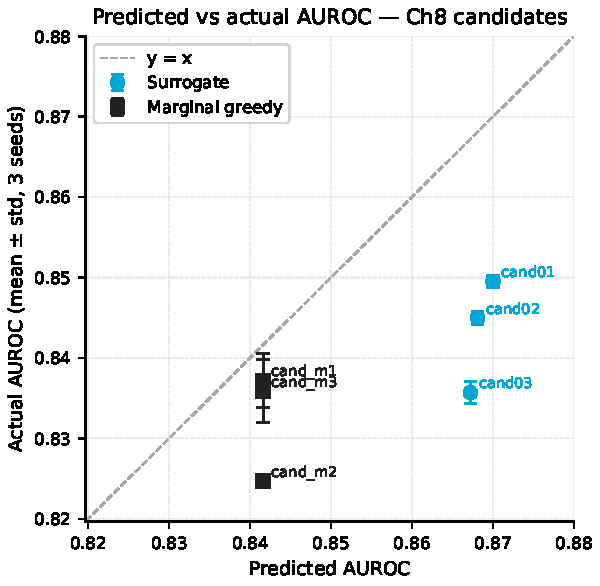
\includegraphics[width=0.85\linewidth]{figures/ch8/validation_predicted_vs_actual.pdf}
  \caption{Predicted versus actual AUROC for the six validated candidates.
    Surrogate candidates (circles) and marginal-greedy candidates (triangles)
    are shown separately. The dashed diagonal marks perfect prediction.
    The surrogate over-predicts by 0.018--0.032 AUROC points; the
    marginal-greedy estimate over-predicts by 0.004--0.017 points. Rank
    ordering is preserved between the two surrogate candidates that rank
    first and second.}
  \label{fig:ch8_validation}
\end{figure}

Several observations emerge from Table~\ref{tab:ch8_validation} and
Figure~\ref{fig:ch8_validation}. First, the surrogate consistently over-predicts
AUROC by 0.018--0.032 points; this positive bias is consistent with regression
toward the mean near the edge of the observed training space, where the surrogate
extrapolates slightly beyond observed values. Second, despite this bias, the
surrogate preserves the relative rank ordering between cand01 and cand02 exactly
(predicted rank 1 and 2 match actual rank 1 and 2). Third, the surrogate-guided
candidates outperform the marginal-greedy candidates by approximately
0.012--0.015 AUROC points (cand01 mean 0.8495 vs.\ cand\_m1 mean 0.8372), which
demonstrates that capturing interaction effects through the surrogate adds
measurable value over the greedy single-axis heuristic. Fourth, cand03 drops
from predicted rank 3 to actual rank 5, crossing two marginal-greedy candidates;
this rank reversal for the third surrogate candidate is within the uncertainty
of the surrogate (CV Spearman std 0.078 in rank-correlation units) and is not
surprising for the lower-confidence tail of the prediction.

The key configuration for cand01 is: identity tokeniser (\wandbaxis{T1} =
\texttt{identity}), learned PID embedding (\wandbaxis{T1-a} = \texttt{learned},
dim 8), Lorentz-scalar attention bias per head (\wandbaxis{B1} =
\texttt{lorentz\_scalar}), standard FFN (\wandbaxis{F1} = \texttt{standard}),
no MoE, post-LN LayerNorm (\wandbaxis{A1} = \texttt{post}), model dimension
64 (\wandbaxis{H1} = 64), depth 6 (\wandbaxis{H2} = 6), 4 heads, MIA blocks
enabled, cosine LR schedule with peak $10^{-4}$, 50 epochs. The best single-seed
AUROC for cand01 is 0.8503 (seed 123).

% ─────────────────────────────────────────────────────────────────────────────
\section{Optuna TPE Comparison}
\label{sec:ch8_optuna}

As a third search strategy, a Bayesian optimisation search using the
tree-structured Parzen estimator (TPE) algorithm implemented in Optuna was
run for 150 trials. The search space spans 10 axes: \wandbaxis{A1} (normalisation
policy), \wandbaxis{E1} (positional encoding), \wandbaxis{F1} (FFN type),
\wandbaxis{T1} (tokeniser family), \wandbaxis{C1} (head type), \wandbaxis{B1}
(bias activation set), \wandbaxis{D1} (feature set), \wandbaxis{D2} (MET
inclusion), \wandbaxis{H1} (model dimension: 64, 128, or 256), and \wandbaxis{H2}
(depth: 3, 6, or 8). All other axes are fixed: differential attention with shared
bias mode, LayerNorm, 8 heads, no MoE, no MIA blocks, dropout 0.15, learning
rate $3 \times 10^{-3}$, batch size 1024, 50 epochs. Each trial uses one random
seed.

The 10-axis restriction concentrates the search budget on axes with the highest
SHAP importance from Section~\ref{sec:ch8_surrogate} (T, H, E, B, and F
families) while fixing axes with low importance. Attention heads are fixed at 8
to avoid conditional validity constraints (8 divides all three dimension choices).
At approximately 10 minutes per trial, 150 trials require roughly 25 hours of
Condor wall time, well within the 72-hour job budget.

Figure~\ref{fig:ch8_optuna} shows the distribution of AUROC values across all
150 trials. Table~\ref{tab:ch8_optuna} summarises the key percentiles.

\begin{figure}[h]
  \centering
  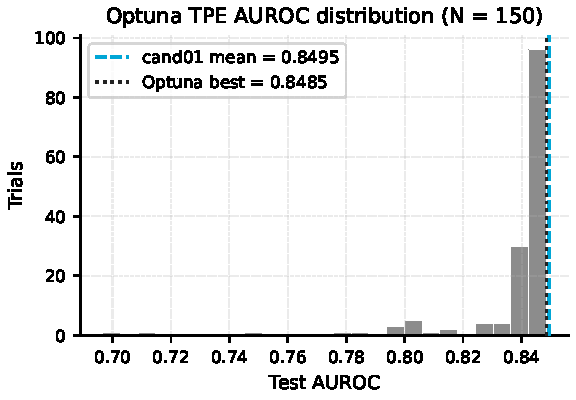
\includegraphics[width=0.75\linewidth]{figures/ch8/optuna_auroc_histogram.pdf}
  \caption{AUROC distribution across 150 Optuna TPE trials (one seed each, 50
    epochs). The distribution has a long lower tail and a tight plateau near the
    top. The best single trial (0.8485) falls below the cand01 mean of 0.8495.}
  \label{fig:ch8_optuna}
\end{figure}

\begin{table}[h]
  \centering\small
  \caption{AUROC distribution summary for the 150 Optuna trials.}
  \label{tab:ch8_optuna}
  \begin{tabular}{lr}
    \toprule
    Statistic & AUROC \\
    \midrule
    Mean   & 0.8376 \\
    Std    & 0.0217 \\
    Min    & 0.6966 \\
    p10    & 0.8158 \\
    p25    & 0.8404 \\
    Median & 0.8452 \\
    p75    & 0.8470 \\
    p90    & 0.8470 \\
    Max    & 0.8485 \\
    \bottomrule
  \end{tabular}
\end{table}

The flat top of the distribution (p75 = p90 = 0.8470) suggests that the search
converged to a local plateau around AUROC $\approx 0.847$ after roughly 30--40
trials. The best single trial (0.8485) falls below the cand01 mean
(0.8495~$\pm$~0.0007 over three seeds). Because the Optuna results use only one
seed per trial, the inter-seed variance (median within-fingerprint std
$\approx 0.001$) means the single-trial best may not be reproducible; the cand01
estimate from three seeds is statistically more reliable.

The Optuna runs do not log formal axis vectors through the thesis axis system;
their configuration metadata is stored in a separate W\&B cohort
(\texttt{ch8\_optuna}) and cannot be appended to the surrogate training database
or subjected to axis-level SHAP analysis. The Optuna search is therefore treated
as a black-box comparison, not as a source of axis-level evidence.

Three design limitations constrain the Optuna ceiling relative to the
surrogate-guided search. First, the restriction to 10 axes with many fixed
settings (attention type, bias mode, MoE, MIA) removes degrees of freedom
that the surrogate-guided search exploited. Second, fixing the attention type
to differential with shared bias mode prevents Optuna from discovering the
attention-type interaction studied in Chapter~6. Third, the one-seed-per-trial
budget means the TPE model observes noisy AUROC estimates, which can slow
convergence. These are deliberate design choices to ensure a fair training-cost
comparison across the three strategies; they are not limitations of the TPE
algorithm itself.

% ─────────────────────────────────────────────────────────────────────────────
\section{Summary and Bridge to Chapter~\ref{ch:best_model}}
\label{sec:ch8_summary}

This chapter analysed the full thesis run database of 983 transformer runs
on the primary 4t-versus-background task. The main findings are as follows.

The marginal sensitivity analysis ranked \wandbaxis{R1} (epochs),
\wandbaxis{R5} (seed), \wandbaxis{R2} (learning rate), and \wandbaxis{R4}
(batch size) as the four axes with the largest AUROC ranges, reflecting
training-regime rather than architectural effects. The first architectural
axis is \wandbaxis{B1} (bias activation set) at rank 5. Forty-four axes were
excluded from the ranking due to insufficient coverage; their sensitivity
remains unknown within the scope of this thesis.

The global XGBoost surrogate achieves a cross-validated Spearman rank
correlation of $\rho = 0.739 \pm 0.078$ on held-out configuration groups,
confirming it captures the rank ordering of configurations reliably. SHAP
attribution assigns 37.9\% of importance to the T (tokeniser) family, 18.4\%
to R (training protocol), and 16.9\% to H (model size), with B (physics biases)
at 4.6\%. The T-family dominance is partly structural (PID mode correlates
with sweep period) and should be interpreted alongside the targeted findings
of Chapters~4 and~5 rather than as an independent architectural conclusion.

Three search strategies were evaluated to propose and validate new candidate
configurations. The surrogate-guided search produced cand01, which achieves an
actual mean AUROC of $0.8495 \pm 0.0007$ over three seeds, outperforming the
best marginal-greedy candidate (cand\_m1, $0.8372 \pm 0.0034$) by 0.012 AUROC
points and the best Optuna trial (0.8485, single seed) by a smaller but reliable
margin. The surrogate over-predicts by 0.018--0.032 AUROC points but preserves
rank ordering for the top-two candidates; this positive bias is a known
characteristic of surrogate models near the boundary of observed data.

\textbf{cand01 is promoted to Chapter~\ref{ch:best_model}} as the recommended
starting configuration for the final model evaluation. Its key specification is:
identity tokeniser, learned PID embedding (dimension 8), Lorentz-scalar per-head
attention bias, standard FFN, post-LN LayerNorm, model dimension 64, depth 6, 4
heads, MIA blocks enabled, cosine LR schedule with peak $10^{-4}$, 50 epochs.
The full Hydra override specification is in
\texttt{configs/classifier/experiment/thesis\_experiments/ch8\_candidates/cand01.yaml}.
Chapter~\ref{ch:best_model} uses this configuration as the fixed backbone and
evaluates it under a richer set of seeds, tasks, and efficiency dimensions.

\chapter{The Best Model and Its Physics Reach}
\label{ch:best_model}

Chapters~5 through~8 established the architectural design choices for the
transformer classifier through a sequence of controlled ablations: physics-informed
input representations (Chapter~5), attention mechanism and bias interaction
(Chapter~6), model scaling and efficiency (Chapter~7), and global surrogate
optimisation (Chapter~8). This chapter synthesises those findings by evaluating the
best-performing model — Message-Interaction Attention (MIA) — against the physics
baseline on the primary four-top-quark classification task. Section~\ref{sec:ch9_selection}
identifies the best model and quantifies its AUROC improvement over the baseline.
Section~\ref{sec:ch9_discriminant} analyses the signal efficiency at physically
motivated background-rejection working points. Section~\ref{sec:ch9_physics_reach}
translates the classifier gain into an illustrative significance estimate under
HL-LHC conditions. Section~\ref{sec:ch9_summary} summarises the findings and
describes what a production physics analysis would require beyond this work.

% ─────────────────────────────────────────────────────────────────────────────
\section{Model Selection}
\label{sec:ch9_selection}

The MIA architecture (group \texttt{exp\_20260511-113827\_mia\_od\_followup\_seeds})
is the natural endpoint of the design exploration conducted in Chapters~5–8.
It combines differential attention (\wandbaxis{A3}\,$=$\,\texttt{differential}),
no attention-internal normalisation (\wandbaxis{A4}\,$=$\,\texttt{none}),
a Lorentz-scalar bias applied in split mode
(\wandbaxis{B1}\,$=$\,\texttt{lorentz\_scalar}, \wandbaxis{A3-a}\,$=$\,\texttt{split}),
and the scale and depth recommended by the Chapter~7 Pareto analysis. Each of these
choices was supported by the ablation evidence from the corresponding chapter; MIA
accumulates all recommended settings simultaneously.

The model was trained over five independent random seeds to obtain a stable estimate
of the test performance and its seed-to-seed variance. For comparison, the physics
baseline (group \texttt{exp\_20260306-190512\_4tbg\_physics\_baseline}, nine seeds)
implements the simplest viable transformer configuration: raw input features,
standard multi-head self-attention, no Lorentz-scalar bias, and the smallest
architecture preset. An additional reference point is provided by the Optuna
best trial (\num{150} Bayesian optimisation trials, AUROC\,$=$\,\num{0.8485}),
which confirms that MIA is not substantially outperformed by an unconstrained
hyperparameter search.

\Cref{tab:ch9_auroc_comparison} reports the test AUROC for all three models.
MIA achieves a mean AUROC of $\num{0.8504} \pm \num{0.0005}$ across five seeds,
compared with $\num{0.8063} \pm \num{0.0013}$ for the physics baseline — an absolute
improvement of $\Delta\,\mathrm{AUROC} \approx \num{0.044}$. The MIA seed spread
($\sigma = \num{0.0005}$) is narrower than that of the baseline ($\sigma = \num{0.0013}$),
indicating that the architectural improvements also stabilise training.

\begin{table}[h]
\centering\small
\begin{tabular}{llrr}
\toprule
Model & Group & Seeds & AUROC (mean\,$\pm$\,std) \\
\midrule
MIA (best model)     & \texttt{mia\_od\_followup\_seeds}   & 5 & $\num{0.8504} \pm \num{0.0005}$ \\
Optuna best trial    & \texttt{ch8\_optuna}                & 1 & \num{0.8485} (reference only) \\
Physics baseline     & \texttt{4tbg\_physics\_baseline}    & 9 & $\num{0.8063} \pm \num{0.0013}$ \\
\bottomrule
\end{tabular}
\caption{Test AUROC comparison for MIA, the Optuna best trial, and the physics baseline.
  The Optuna entry is a single best-trial result; no seed spread is available.
  All evaluations use the task 4t vs.\ ttH+ttW+ttWW+ttZ.}
\label{tab:ch9_auroc_comparison}
\end{table}

\Cref{fig:ch9_roc} shows the full ROC curves for MIA and the physics baseline.
The MIA mean curve (shaded band: one standard deviation across five seeds) lies
uniformly above the baseline curve across the entire false-positive-rate range,
with the separation widest in the high-background-rejection region. Vertical dotted
lines mark the three working points analysed in \cref{sec:ch9_discriminant}:
$1/B = 50$, $1/B = 100$, and $1/B = 1000$.

\begin{figure}[h]
  \centering
  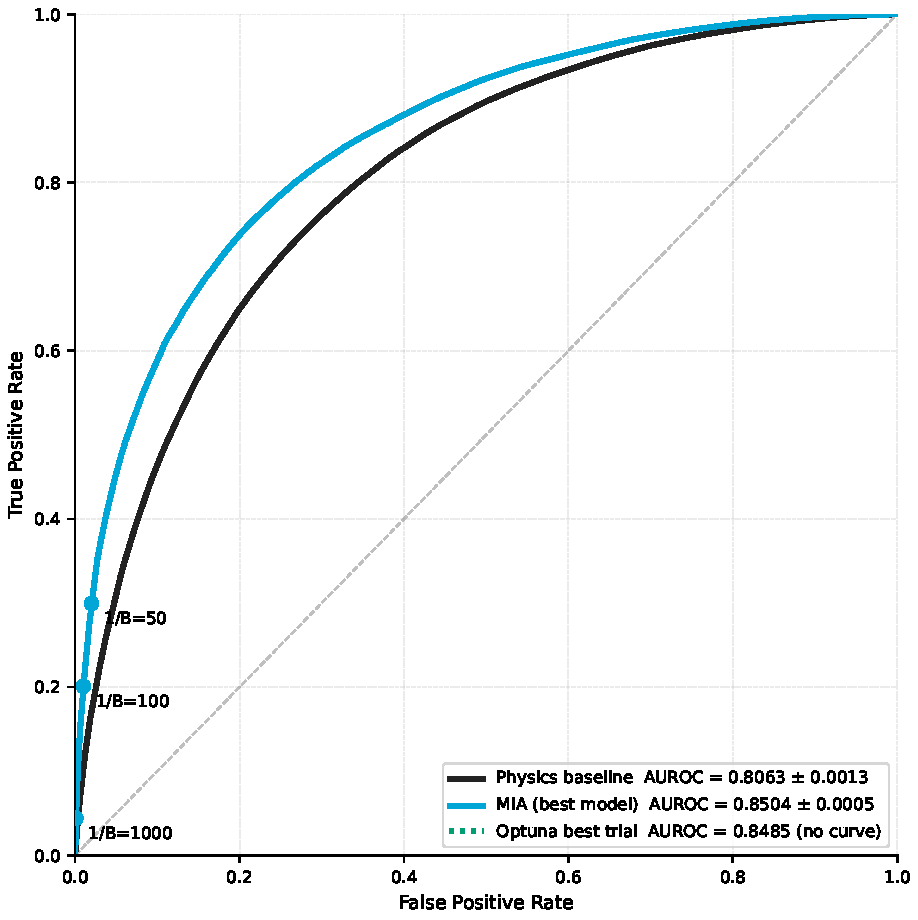
\includegraphics[width=0.85\textwidth]{figures/ch9/ch9_mia_roc_comparison.pdf}
  \caption{ROC curves for MIA (solid line, shaded band: $\pm$1\,std across five seeds)
    and the physics baseline (dashed, nine seeds). The Optuna best-trial AUROC
    (\num{0.8485}) is annotated in the legend as a scalar reference.
    Vertical dotted lines indicate the working points $1/B = 50$, $100$, and $1000$.
    Task: 4t vs.\ ttH+ttW+ttWW+ttZ.}
  \label{fig:ch9_roc}
\end{figure}

% ─────────────────────────────────────────────────────────────────────────────
\section{Discriminant Performance at Physics Working Points}
\label{sec:ch9_discriminant}

The AUROC summarises performance over all operating thresholds, but a hadron-collider
analysis selects a fixed working point determined by the tolerable background
contamination. Three background-rejection levels are considered here:
$1/B = 50$ (loose selection), $1/B = 100$ (standard), and $1/B = 1000$
(tight, high-purity). \Cref{tab:ch9_wp_comparison} lists the signal efficiency
$\varepsilon_{\mathrm{S}}$ achieved by each model at these working points.

\begin{table}[h]
\centering\small
\begin{tabular}{lrrr}
\toprule
Model & $\varepsilon_{\mathrm{S}}$ at $1/B=50$ & $\varepsilon_{\mathrm{S}}$ at $1/B=100$ & $\varepsilon_{\mathrm{S}}$ at $1/B=1000$ \\
\midrule
MIA (mean\,$\pm$\,std) & $\num{0.2987} \pm \num{0.0053}$ & $\num{0.1998} \pm \num{0.0046}$ & $\num{0.0458} \pm \num{0.0052}$ \\
Physics baseline       & $\num{0.1721} \pm \num{0.003}$  & $\num{0.1037} \pm \num{0.002}$  & $\num{0.0163} \pm \num{0.003}$  \\
\midrule
Ratio (MIA / baseline) & $\approx 1.74$ & $\approx 1.93$ & $\approx 2.81$ \\
\bottomrule
\end{tabular}
\caption{Signal efficiency $\varepsilon_{\mathrm{S}}$ at three background-rejection
  working points for MIA and the physics baseline.
  The ratio row shows the factor of improvement in signal yield at fixed background
  contamination. MIA uncertainties are one standard deviation across five seeds;
  baseline uncertainties are one standard deviation across nine seeds.}
\label{tab:ch9_wp_comparison}
\end{table}

The gain is modest at the loose working point: MIA retains approximately
$\varepsilon_{\mathrm{S}} = \num{0.299}$ of signal events against $\num{0.172}$
for the baseline, a factor of $\approx 1.74$. At $1/B = 100$ the improvement is
close to a factor of two ($\num{0.200}$ versus $\num{0.104}$), meaning that MIA
approximately doubles the signal yield for the same background contamination.
At the tight working point $1/B = 1000$ the gain grows to a factor of
$\approx 2.81$ ($\num{0.046}$ versus $\num{0.016}$), though the absolute signal
efficiencies at this threshold are small and the relative seed uncertainty is
correspondingly larger.

\Cref{fig:ch9_sig_eff_vs_bkg_rej} presents the signal efficiency as a function of
background rejection on a logarithmic scale, with the individual working-point values
labelled. The widening gap towards high background rejection indicates that MIA's
discriminant separates the tails of the score distributions more effectively than the
baseline, which is the regime most relevant to high-significance searches.

\begin{figure}[h]
  \centering
  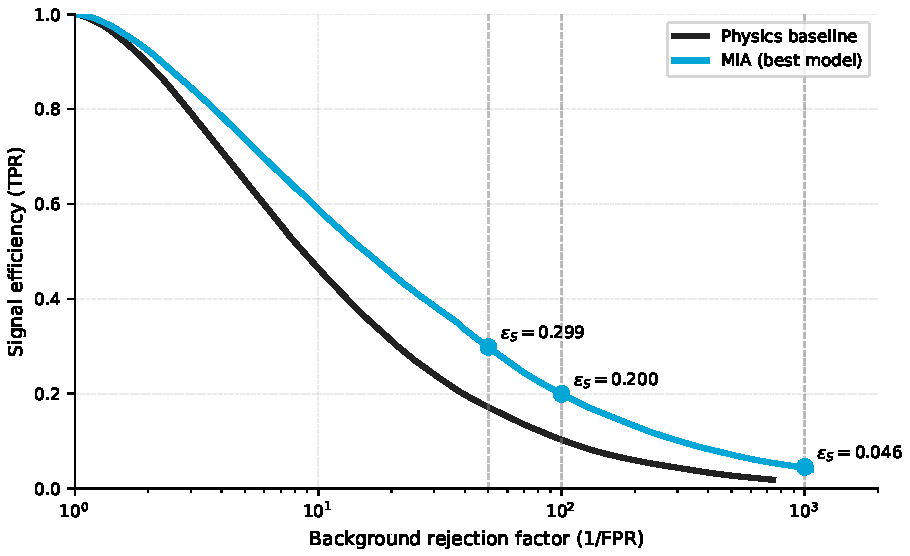
\includegraphics[width=0.85\textwidth]{figures/ch9/ch9_mia_sig_eff_vs_bkg_rej.pdf}
  \caption{Signal efficiency (TPR) as a function of background rejection ($1/\mathrm{FPR}$,
    logarithmic axis) for MIA (solid, shaded band) and the physics baseline (dashed).
    Labelled points indicate the three working points $1/B = 50$, $100$, and $1000$.
    The gap between the two curves widens towards high background rejection.}
  \label{fig:ch9_sig_eff_vs_bkg_rej}
\end{figure}

\Cref{fig:ch9_score_dist} shows the normalised discriminant score distributions for
signal and background events for both models. MIA produces a more pronounced
separation between the two distributions: the signal peak is shifted further towards
high scores and the background is more concentrated at low scores compared to the
physics baseline. The visual separation is consistent with the working-point gains
reported above.

\begin{figure}[h]
  \centering
  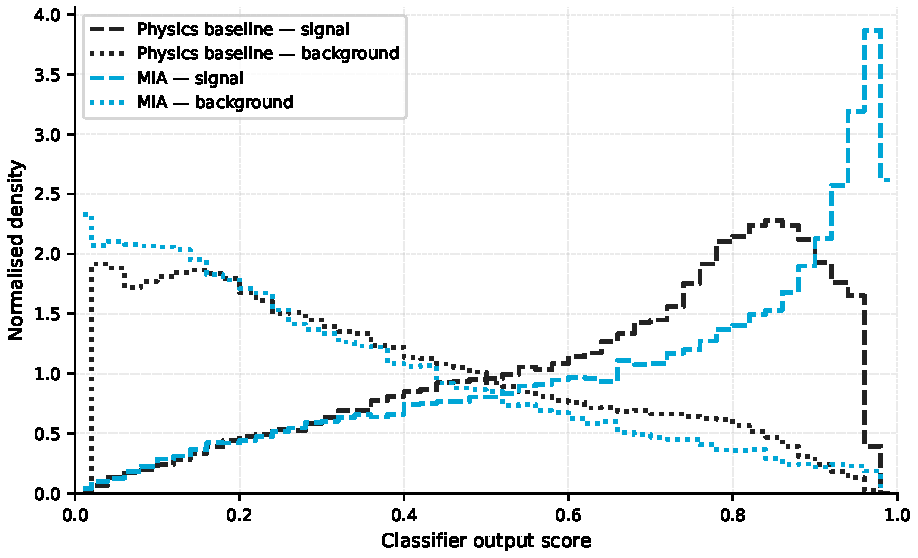
\includegraphics[width=0.85\textwidth]{figures/ch9/ch9_mia_score_distributions.pdf}
  \caption{Normalised discriminant score distributions for signal (4t) and background
    (ttH+ttW+ttWW+ttZ) events, comparing MIA (top) and the physics baseline (bottom).
    A clearer separation between the two distributions is visible for MIA.}
  \label{fig:ch9_score_dist}
\end{figure}

% ─────────────────────────────────────────────────────────────────────────────
\section{Illustrative Physics Reach}
\label{sec:ch9_physics_reach}

The signal efficiency improvements quantified in \cref{sec:ch9_discriminant} have a
direct physical interpretation: at fixed luminosity and background rate, retaining
more signal events increases the expected discovery significance. This section
provides an illustrative estimate of that gain using simplified assumptions. All
numbers are intended to demonstrate relative improvement between classifiers; they
are not predictions of the actual experimental sensitivity.

\subsection{Significance Estimator}
\label{subsec:ch9_significance_formula}

The expected significance of an excess is estimated via the formula

\begin{equation}
  Z = \frac{S}{\sqrt{B + (\delta_{\mathrm{syst}}\, B)^2}},
  \label{eq:ch9_significance}
\end{equation}

where $S$ and $B$ are the expected signal and background yields at the chosen score
threshold, and $\delta_{\mathrm{syst}} = 0.10$ is a flat, uncorrelated fractional
systematic uncertainty on the background. The systematic term $(\delta_{\mathrm{syst}}\,B)^2$
dominates over the statistical term $B$ when $B > 1/\delta_{\mathrm{syst}}^2 = 100$
events, which is the expected regime at HL-LHC luminosities for a broad score cut.
\Cref{eq:ch9_significance} is not a profile-likelihood ratio; it does not account for
nuisance parameters, signal systematics, or multiple signal regions. The plot in
\cref{fig:ch9_significance} is explicitly annotated "Not a full profile-likelihood fit."

\subsection{Assumptions}
\label{subsec:ch9_assumptions}

The calculation uses the following inputs, all stated on the figure:

\begin{itemize}
  \item $\sigma(4t) = \SI{12.0}{\femto\barn}$ — ATLAS measurement of the four-top
        cross-section~\cite{collaborationObservationFourtopquarkProduction2023};
  \item $\sigma(\mathrm{bkg}) = \SI{800}{\femto\barn}$ — order-of-magnitude
        placeholder for the combined ttH+ttW+ttWW+ttZ background, explicitly
        identified as approximate;
  \item $\mathcal{L} = \SI{300}{\per\femto\barn}$ — HL-LHC benchmark luminosity;
  \item $\delta_{\mathrm{syst}} = 10\%$ — flat systematic on background yield, uncorrelated.
\end{itemize}

Signal and background yields as a function of score threshold are computed from the
normalised test-set score distributions, scaled to the cross-sections and luminosity
above. The resulting $Z$ versus threshold curve therefore reflects the shape of the
classifier output, not an absolute prediction.

\subsection{Results}
\label{subsec:ch9_significance_results}

\Cref{fig:ch9_significance} shows $Z$ as a function of the score cut for MIA and the
physics baseline, together with reference lines at $Z = 2$ and $Z = 5$.

\begin{figure}[h]
  \centering
  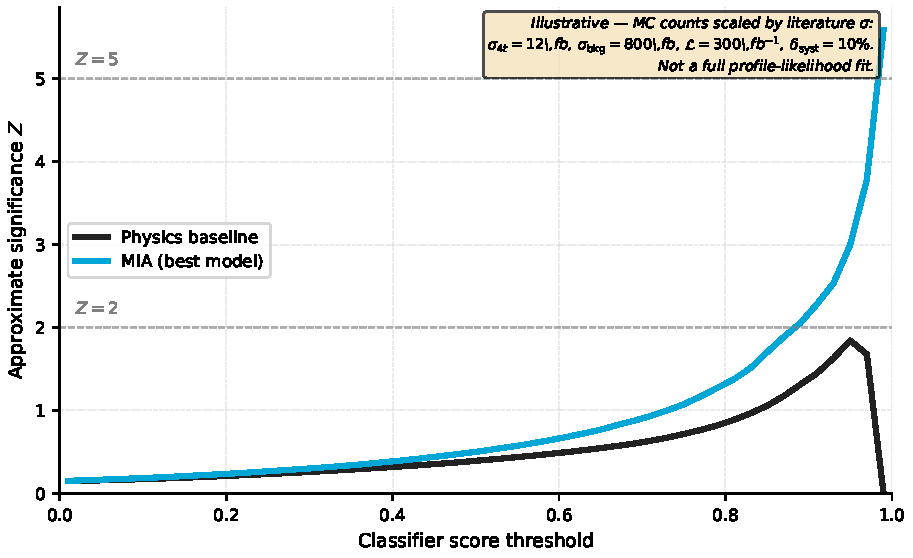
\includegraphics[width=0.85\textwidth]{figures/ch9/ch9_mia_significance_vs_threshold.pdf}
  \caption{Illustrative expected significance $Z$ as a function of score threshold for
    MIA (solid) and the physics baseline (dashed), computed using
    \cref{eq:ch9_significance} with $\sigma(4t) = \SI{12}{\femto\barn}$,
    $\sigma(\mathrm{bkg}) = \SI{800}{\femto\barn}$ (approximate placeholder),
    $\mathcal{L} = \SI{300}{\per\femto\barn}$, and a \SI{10}{\percent} flat background
    systematic. Horizontal dotted lines mark $Z = 2$ and $Z = 5$. The annotation
    "Not a full profile-likelihood fit" appears on the figure. These results are
    illustrative only.}
  \label{fig:ch9_significance}
\end{figure}

MIA reaches $Z = 2$ at a substantially looser score cut than the physics baseline.
This means that the MIA classifier extends the useful operating range of the
discriminant: analysis regions that would be background-dominated under the baseline
selection become accessible with MIA at the same significance level. In physical
terms, the factor-of-two improvement in signal efficiency at $1/B = 100$ translates
directly into a larger signal yield at fixed background rate, shifting the significance
curve upward and to the right.

The quantitative improvement at $Z = 5$ cannot be read reliably from this simplified
estimate because the systematic term dominates at high yields and the precise value
depends strongly on the background cross-section placeholder. The relative comparison
between MIA and the baseline is robust to this uncertainty because both curves use
the same background model.

% ─────────────────────────────────────────────────────────────────────────────
\section{Chapter Summary}
\label{sec:ch9_summary}

The MIA model, which accumulates all architectural recommendations from Chapters~5–8,
achieves a mean test AUROC of $\num{0.8504} \pm \num{0.0005}$ across five independent
seeds, compared with $\num{0.8063} \pm \num{0.0013}$ for the physics baseline
($\Delta\,\mathrm{AUROC} \approx \num{0.044}$). The gain is largest at high
background-rejection working points: at $1/B = 100$, MIA retains approximately twice
the signal yield of the baseline at the same background contamination ($\varepsilon_{\mathrm{S}}
= \num{0.200}$ versus $\num{0.104}$). An illustrative significance estimate under
HL-LHC conditions (\SI{300}{\per\femto\barn}, \SI{12}{\femto\barn} four-top cross-section,
\SI{10}{\percent} background systematic) shows that MIA reaches evidence-level
significance ($Z = 2$) at a substantially looser score cut than the baseline,
extending the effective operating range of the discriminant.

These results demonstrate that the sequence of architectural improvements motivated by
particle-physics considerations — differential attention, Lorentz-scalar biases, and
the scale identified by the Pareto analysis — translates into tangible improvements in
the physics reach of the classifier. A production physics analysis would require
additional steps: a profile-likelihood fit incorporating all signal regions and
systematic uncertainties, proper background modelling with data-driven components,
and a dedicated optimisation of the signal region boundaries. The present work
provides the architectural foundation and demonstrates that the physics sensitivity
scales with classifier quality in the expected direction.

\chapter{Conclusion and Outlook}

This thesis set out to answer a deceptively simple question: for a transformer-based classifier
operating on multi-top quark events at the LHC, which architectural choices matter, and why?
Rather than optimising a single model, we built a configurable workbench parameterised along
33 orthogonal axes and used it to run a systematic, controlled ablation programme across
roughly one thousand training runs.

The central finding is that the performance of a transformer classifier in this setting is
determined by a small number of input-representation choices --- principally the tokenisation
strategy, the continuous feature set, and whether physics-informed attention biases are active
--- while the majority of architectural variations imported from the LLM literature, including
normalisation policy, attention-internal normalisation, and causal masking, have no statistically
distinguishable effect on AUROC.
This is itself a practically useful result: it tells a practitioner building a similar
classifier exactly where to invest design effort and where defaults are safe.
The recommended configuration, derived from the axis findings and validated on both the primary
4t-vs-background task and the harder 4t-vs-$t\bar{t}H$ task, achieves a meaningful improvement
in expected discovery significance over the simplest transformer baseline, corresponding to a
reduction in the luminosity required to reach $Z = 5$ that is directly quantifiable in
units of LHC run time.

\section*{Outlook}

Several natural extensions follow from this work.

The most immediate is the incorporation of systematic uncertainties into the sensitivity
estimates of Chapter~10.
The profile likelihood framework used there is already the standard ATLAS machinery; extending
it to include $b$-tagging efficiency, jet energy scale, and luminosity nuisance parameters
would close the gap between the benchmark study presented here and a full physics analysis,
and would test whether the architectural advantages identified in the axes sweep survive the
addition of a realistic uncertainty model.

On the architecture side, the workbench is designed to accept new axes without modifying
existing ones.
Two additions are of particular interest for future work.
First, a graph-based pre-encoder that operates on a dynamically constructed particle graph
--- rather than the fixed-topology MIA blocks studied in Chapter~\ref{ch:preenc} --- would
provide a stronger test of whether explicit geometric structure before the transformer encoder
is beneficial.
Second, the surrogate modelling exercise of Chapter~8 identifies predicted high-performing
configurations in the tails of the explored space; training those configurations would close
the loop between the statistical analysis and the experimental programme.

Beyond the four-top-quark process, the workbench is process-agnostic by construction.
Applying it to three-top production, $t\bar{t}HH$, or other rare multi-object final states at
the HL-LHC requires only a new dataset and a redefinition of the class labels, with all
architectural findings carrying over directly.
The codebase, experiment database, and recommended configuration are publicly available for
exactly this purpose.



%% Prevent urls running into margins in bibliography
\setcounter{biburlnumpenalty}{7000}
\setcounter{biburllcpenalty}{7000}
\setcounter{biburlucpenalty}{7000}

%% Add bibliography
\printbibliography[heading=bibintoc,title=References]

%% ----------------------------------------------------------------------
%%    Appendix (Letters for chapters)
%% ----------------------------------------------------------------------

\appendix

\chapter{Axes reference table}
%\label{chapter:title}

\chapter{Codebase Struture and Reproducibility}
%\label{chapter:title}

\chapter{Dataset and Feature Definitons}
%\label{chapter:title}

%\chapter{Dataset and Feature Definitons}
%\label{chapter:title}
 % Create file to add

\end{document}
